\documentclass[12pt]{article}
\usepackage[utf8]{inputenc}
\usepackage{xcolor}
%\usepackage{mdframed}% for framed figures
%\colorlet{framecolor}{gray}

\usepackage{natbib} 
\usepackage{ulem}%for strike through, can be deleted when submitting the paper
%\usepackage[backend=bibtex, style=authoryear]{biblatex} %compile on this order --> LaTeX BiBTeX LaTeX
%\addbibresource{refs.bib}
\usepackage{amsmath,amsthm,amsfonts,dsfont}
\usepackage{mathrsfs}  
\usepackage{tikz}
\usepackage{amssymb}
\usepackage{fullpage}
\usepackage{tabularx}
\usepackage[hidelinks]{hyperref}
\usepackage{float}
\usepackage{subfigure}
\newtheorem{theorem}{Theorem}[section]
\newtheorem{property}[theorem]{Property}
\newtheorem{corollary}[theorem]{Corollary}
\newtheorem{lemma}[theorem]{Lemma}
\theoremstyle{definition}
\newtheorem{definition}{Definition}[section]
\theoremstyle{remark}
\newtheorem*{remark}{Remark}


\usepackage[inline]{enumitem}

\newcommand{\restrict}{\mid}
\newcommand{\range}[1]{\mathscr{#1}}

%%%%%%%%%%%%%%%%%%%%%%%%%%%%%%%%%% Greek
\newcommand{\zdistparama}{\alpha}
\newcommand{\zdistparamb}{\beta}
\newcommand{\zdistparamc}{\gamma}
\newcommand{\freeGamma}{\Gamma}
\newcommand{\order}{\delta}
\newcommand{\freeDelta}{\Delta}

\newcommand{\dominantU}{\nu}
\newcommand{\dominantUbar}{\bar{\nu}}
\newcommand{\sampledensity}{\mathbf{\pi}}
\newcommand{\intensity}{\lambda}
\newcommand{\Intensity}{\Lambda}
\newcommand{\dominantY}{\eta}
\newcommand{\dominantYbar}{\bar{\eta}}
\newcommand{\intensityratio}{\rho}
\newcommand{\densityratio}{\rho}
\newcommand{\parampop}{\theta}
\newcommand{\permutation}{\tau}
\newcommand{\paramnuisance}{\xi}
\newcommand{\provar}{\Sigma}
\newcommand{\Residual}{\varepsilon}
%\newcommand{\Covf}{\Gamma}
%%%%%%%%%%%%%%%%%%%%%%%%%%%%%%%%%% Latin

\newcommand{\acos}{acos}
\newcommand{\subsetA}{A}
\newcommand{\Covariogram}{C}
\newcommand{\Cov}{\mathrm{Cov}}
\newcommand{\derive}{\mathrm{d}}
\newcommand{\Design}{D}
\newcommand{\design}{\mathbf{d}}
\newcommand{\E}{\mathrm{E}}
\newcommand{\density}{\mathrm{f}}
\newcommand{\Semivariogram}{G}
\newcommand{\indicator}{I}
\newcommand{\Sampleindex}{K}
\newcommand{\sampleindex}{\mathbf{k}}
\newcommand{\likelihood}{\mathscr{L}}
%\newcommand{\popsize}{N}
\newcommand{\Samplesize}{N}
\newcommand{\samplesize}{\mathbf{n}}
%\newcommand{\P}{P}
\newcommand{\Sample}{S}
\newcommand{\sample}{\mathbf{s}}
\newcommand{\size}{\mathrm{size}}
\newcommand{\Pop}{\mathrm{U}}
\newcommand{\toPop}{\bar{\mathrm{U}}}
\newcommand{\Var}{\mathrm{Var}}
\newcommand{\Position}{X}
\newcommand{\position}{\mathbf{x}}
\newcommand{\SignalSpace}{\mathscr{Y}}
\newcommand{\toSignalSpace}{\bar{\SignalSpace}}
\newcommand{\Signal}{Y}
\newcommand{\signal}{\mathbf{y}}
\newcommand{\Desvar}{Z}
\newcommand{\DesvarSpace}{\mathscr{Z}}
\newcommand{\desvar}{\mathbf{z}}

\newcommand{\xxx}{.5}
\newcommand{\yyy}{.5}
\newcommand{\hhh}{.5}
\newcommand{\xx}[1]{\renewcommand{\xxx}{#1}}
\newcommand{\hh}[1]{\renewcommand{\hhh}{#1}}
\newcommand{\yy}[1]{\renewcommand{\yyy}{#1}}

\newcommand\smallplot{
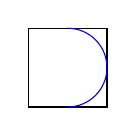
\begin{tikzpicture}
    \draw (0, 0) rectangle (1, 1);
    \draw[blue] (\xxx,\yyy+\hhh) arc(90:-90:\hhh);
  \end{tikzpicture}}

\title{Informative Selection and Spatial Process}
\date{}
\author{Bonn\'ery,  Pantalone, Ranalli}
\begin{document}
\normalem %delete this line when ulem packages is removed

\maketitle

\tableofcontents

\begin{abstract}
This paper extends the concept of informative selection, population distribution and sample distribution in a spatial process context.
Those notions were defined by 
\cite{pfefferman_1992} in a context where the output of the random process of interest consists of independent and identically distributed realisations for each individuals of a population. \cite{BonneryBreidtCoquet} showed that informative selection was inducing a stochastic dependence among realisations on the selected units. In the context of spatial process, the "population" is a continuous space and realisations for two different elements of the population are not independent. We show how informative selection may induce a different dependence among selected units, how the sample distribution differs from the "population" distribution, and how one can  account for this effect in an simulated study when doing statistical inference, including Semi-variogram parametric and semi parametric estimation, as well as prediction on the part of the space for which the random process was not observed.
\end{abstract}

{\color{red} The references in abstracts should be either written in full or not given}.

\section{Intro}

\section{Introduction} \label{sec:intro}
Spatial processes are employed in many fields, such as geology, Earth science, environmental and agricultural surveys, among many others. A large variety of data is surveyed in space, such as rainfall \citep{ord1979spatial}, atmospheric  \citep{thiebaux1987spatial}, forestry  \citep{samra1989spatial} and soil data \citep{burgess1980optimal}, in order to perform statistical inference on parameters of interest. In these applications, a general approach is to postulate a spatial process for the variable $\Signal$ under investigation, that is a stochastic process is assumed to have generated the population values, also called \emph{superpopulation} model. %Such process is usually parametric, i.e. characterized by a finite number of parameters $\boldsymbol{\theta}$, and the interest is on inference about such parameters. If we use sample data in order to make inference about $\boldsymbol{\theta}$,
When using sample data, we need to pay attention to the relation between the spatial process and the  selection mechanism. Indeed, the distribution of the observed data can be different from the distribution assumed for the population by means of the spatial process $P^{\Signal}$. In other words, the density obtained by the sample data may not be the density obtained by reducing the number of terms in $P^{\Signal}$, as if the units were selected completely at random. In this case, we say that the sampling is \emph{informative}. Ignoring an informative sample may lead to bias and erroneous inference, as illustrated for example in \cite{skinner1989analysis}. This could happen when there is dependence between the assumed stochastic model and the sampling mechanism, that is the units are selected dependently to the variable of interest. Examples of this type of mechanism selection are, among many others, length-biased sampling, endogenous stratification, adaptive sampling, sequential quota sampling, and cut-off sampling. For more details, see Section 3 of \cite{bonnery2012uniform}.

In this paper, we study the effect of informative selection when a spatial process is employed. We consider informative selection as a situation where the sample responses, \emph{given that they were selected}, are not i.i.d. from the superpopulation model. We start from the notion of population and sample distribution defined by \cite{pfefferman_1992}, and we extend those to a spatial process context. Indeed, \cite{pfefferman_1992} consider realizations of a random process of interest as independent and identically distributed, whereas we address the dependence between the realizations, which very likely characterizes a spatial process. As in \cite{pfeffermann1998parametric}, we start from the distribution of the observed values given they were selected, or \emph{sample pdf}. While \cite{pfeffermann1998parametric} consider the observations as if they were independently distributed according to the sample pdf, our work considers the dependence between the observed units in order to account for the spatial component of the population. Also, while \cite{pfeffermann1998parametric} assume that the target population $U$ is finite, our work can be applied to both finite population and continuous populations.

Throughout the paper we assume to have a spatial Gaussian process and a point process that represents the selection mechanism. Given these two processes, we then define the probability density function of the sample and a subsample, and the ``sample'' and ``population'' distribution of the signal. These concepts are needed in order to introduce a \emph{density ratio} that we use for investigating the bias possibly introduced by the selection mechanism, or \emph{selection bias}. In doing that, the spatial structure of the population is taken into account.

These general definitions allow us to define the sample counterpart of different characteristics of the population distribution. Indeed, we focus on the \emph{variogram}, which analyzes the degree of spatial dependence of spatial processes and provides useful insights on the phenomenon under investigation. For instance, the variogram is the key component for the well-known \emph{kriging} method \citep{matheron1962traite}, and it plays a crucial role on prediction since it is used to compute the kriging weights. We introduce the definitions of \emph{population variogram} and \emph{sample variogram}, and we investigate the behaviour of the \emph{naive} estimator, i.e. the estimator that does not take into account the informativeness of the selection mechanism.
%In this paper, we study the effect of informative selection when the variogram is of interest. We consider informative selection as a situation where the sample responses, given that they were selected, are not i.i.d. from the superpopulation model. As in \cite{pfeffermann1998parametric}, we start from the distribution of the observed values given they were selected, or \emph{sample pdf}. The major difference in our approach is that, while \cite{pfeffermann1998parametric} consider the observations as if they were independently distributed according to the sample pdf, our work consider the dependence between the observed units. {\color{red}Indeed, \cite{pfeffermann1998parametric}  }We provide a theoretical background for the definitions of \emph{population variogram} and \emph{sample variogram}, and some properties of the \emph{naive} estimator, i.e. the estimator that does not take into account the informativeness of the selection mechanism.


The paper is organized as follow. In Section \ref{sec:stat_fra} we define the statistical framework used throughout the paper. In particular, general notions and the concepts of spatial process, sample, design and design variables are introduced. In Section \ref{sec:sampledistribution} the sample distribution and the population distribution are defined, and in Section \ref{sec:estimation} estimation of the variogram is briefly reviewed and a  simulation study is carried out in order to investigate the behaviour of the naive estimator. In Section \ref{sec:prediction} we provide the formula for the predictive distribution of the signal conditioned to observed values. Finally, Section \ref{sec:conclusions} provides conclusion and future research.

% The \emph{sample pdf} is defined as the conditional distribution of the random variable $\Signal$ given that it was selected. \cite{pfeffermann1998parametric} use a sample likelihood approach to inference for the superpopulation model, where the product of the sample pdfs is maximized, as if the responses were iid.

%The major approaches to analytic inference from survey data are all based on the likelihood concept. The maximum \emph{full-information} likelihood approach defines the likelihood as the probability of observing all the relevant data available \citep{breckling1994maximum} and the process that has to be accounted for is given by the joint distribution of the spatial process $\Signal$ and the selection mechanism, while the maximum \emph{sample-likelihood} focuses on the distribution of $\Signal$ given it was observed \citep{krieger1992maximum, pfeffermann1993role, pfeffermann1998parametric, pfeffermann1999parametric}, and if this conditional distribution differs from the marginal distribution of $\Signal$, selection bias is introduced and the mechanism selection is \emph{informative}.
 %Since just a portion of the population is observed, the relevant likelihood is given by $P^{I_{U},\Signal_{S}}=\int{P^{I_{U},\Signal_{U}}d\Signal_{U \backslash s}}$, which is usually different from $P^{S}=\int{P^{\Signal_{U}}d\Signal_{U \backslash s}}$.

%The major approaches to analytic inference from survey data are all based on the likelihood concept. The maximum \emph{full-information} likelihood approach defines the likelihood as the probability of observing all the relevant data available \citep{breckling1994maximum}. The process that has to be accounted for is given by the joint distribution of the spatial process $\Signal$ and the selection mechanism.%Since just a portion of the population is observed, the relevant likelihood is given by $P^{I_{U},\Signal_{S}}=\int{P^{I_{U},\Signal_{U}}d\Signal_{U \backslash s}}$, which is usually different from $P^{S}=\int{P^{\Signal_{U}}d\Signal_{U \backslash s}}$.
% \\ The maximum \emph{sample-likelihood} focuses on the distribution of $\Signal$ given it was observed \citep{krieger1992maximum, pfeffermann1993role, pfeffermann1998parametric, pfeffermann1999parametric}. If this conditional distribution differs from the marginal distribution of $\Signal$, selection bias is introduced and the mechanism selection is \emph{informative}.


\section{Statistical Framework} \label{sec:stat_fra}
This section illustrates the concepts and notations defined in \cite{dbb1}.
\subsection{General notations}

In this paper, all random variables are defined on a probability space $(\Omega,\mathscr{A},P)$. The expected value and variance/covariance operators are defined with respect to the probability measure $P$. 
For two sets $E$ and $F$, $(E\to F)$ or $F^E$ designate the set of the functions from $E$ to $F$.
The notation "$g:E\to F,x\mapsto g(x)$" means: let $g$ be a mapping from set $E$ to set $F$ that to $x$ associates $g(x)$. For $f:E\to (F\to G)$, $g:E\to F$, $h:E\to (H\to F)$,  the notation $f[g]$ designates the function :  $f[g]:E\to G$, such that $f[g](x)=(f(x))(g(x))$, and the notation 
$f[h]$ designates the function :  $f[h]:E\to (H\to G)$, such that $f[h](x)=(f(x)\circ h(x))$.


For a set $E$, $\bar{E}$ designates the set $\{\mathbf{0}\}\cup\bigcup_{n\in\mathbb{N},n\geq 1} E^{\{1,\ldots,n\}}$, where $\mathbf{0}=E^\emptyset$ corresponds to the set containing an application with empty domain.
Let denote by $\size $ the application that maps an application to the cardinality of its domain: $\bar{E}\to\mathbb{N}$, $\mathbf{e}\mapsto n$ if $\position\in E^{\{1,\ldots,n\}}$, $0$ if $\position=\mathbf{0}$. For an application $\position\in\bar{E}$, a set $\Sampleindex$, $\position_\Sampleindex$ is the application:
$\position_\Sampleindex:\Sampleindex\cap\mathrm{domain}(\position)\to E:\ell\mapsto\position(\ell)$, in the case of a random application $\Sample:\Omega\to\toPop$ and a random set :$\Sampleindex\to(\mathscr{P}(\mathbb{N})$ ($\mathscr{P}(\mathbb{N})$ is the set of all subsets of $\mathbb{N}$), then $\Sample_\Sampleindex$ is the random application: $\Omega\to\toPop, 
\omega\mapsto 
\Sample_\Sampleindex(\omega):(\Sampleindex(\omega)\cap\mathrm{domain}(\Sample(\omega))\to \Pop),
\ell\mapsto (\Sample(\omega))(\ell)$.
For a measure $\eta$ of $E$, a non random finite set $\Sampleindex$, $\eta^{\otimes\Sampleindex}$ is the measure such that for any collection $(\subsetA_\ell)_{\ell\in\Sampleindex}$ of subsets of $E$  :
$\eta^{\otimes\Sampleindex}\left(\bigcap_{\ell\in\mathbb{L}}\{\position\in E^\Sampleindex:\position(\ell)\in\subsetA_\ell\}\right)=\prod_{\ell\in\Sampleindex}\eta(\subsetA_\ell)$, and
$\eta^{\otimes\emptyset}(\{\mathbf{0}\})=1$, 
then define the measure $\bar{\eta}$ on $\bar{E}$: $\bar{\eta}=\eta^{\otimes\emptyset}+\sum_{\samplesize\in\mathbb{N},\samplesize\geq 0}\eta^{\otimes\{1,\ldots,\samplesize\}}$.

\subsection{Spatial process}
We consider a space $\Pop$, that is a compact (non necessarily convex) subset of a finite dimensional real vector space $\mathbb{R}^d$, with its associated Borel sigma-field, and a random process $\Signal$ defined on $\Pop$ with value in another finite dimension real vector space $\SignalSpace$, e.g. $Y:\Omega\to(\Pop\to\SignalSpace)$.
 For example for a random variable $\Sample:\Omega\to\Pop^{\{1,2\}}$, and a random variable
$\Signal:\Omega\to(\Pop\to\SignalSpace)$, 
$\Signal[\Sample]$ is the random variable: $\Signal[\Sample]:\Omega\to(\{1,2\}\to\SignalSpace)$, $\omega\mapsto(\Signal(\omega))(\Sample(\omega)):\ell\to(\Signal(\omega))(\Sample(\omega)(\ell)$.
The set of all functions 
All definitions will be given under the general statistical framework described above. Examples and illustrations will be given for the particular case where $\Pop=[0,1]^2$.
%Given data $(\position(1),\signal_{1}),...,(\position_{n},\signal_{n})$, in order to perform inference for some target, we postulate a model, which we assume holds for the entire population. In particular, we are interested in model parameters, in other words we focus on \emph{analytic inference}. The choice of the model is not an easy task. It should reflect the structure of the population and should capture the important features useful for inference purpose. An entire branch of literature is dedicated to this task, i.e. \emph{model selection}, but the focus of this paper does not lie in that. 
%For our work we assume that the model describing the variable of interest is given by
%\begin{equation} \label{eq:model}
%\Signal\left[\position\right]=S\left[\position\right]+\epsilon\left[\position\right]
%\end{equation}
%{\color{red} S is for $\Sample$ (sample)}
%where $S\left(\position\right)$ is a zero mean stationary stochastic process in $\mathbb{R}^d$ and is independent from the $\epsilon\left(\position\right)$, which has normal distribution with mean 0 and variance $\sigma_{\epsilon}$. The model in \eqref{eq:model} is quite general and embraces many variations under its umbrella. It is wide known in the field of geostatistics, where the term \emph{kriging} is in vogue. In fact, according to different assumptions about $S(\position)$, we end up with different models, which are usually referred with terms as ordinary kriging, simple kriging, universal kriging and so on. In order to perform inference about the model parameters, we need to introduce some assumptions.
Let $\dominantY$ (resp. $\dominantU$) denote a sigma-finite measure on the set $\SignalSpace$ (resp. $\Pop$).
The notation $\density_{V\mid W}$ denotes the density of $V$ conditional on $W$ with respect to a dominating measure on the domain of $V$.
The average theoretical semivariogram is defined as the function: 
\begin{equation}\Semivariogram:\mathbb{R}^d\to[0,+\infty),h\mapsto\frac12\int_{\Pop^{\{1,2\}}} \Var\left[\Signal[\position(2)]-\Signal[\position(1)]\right] \derive(\dominantU^{\otimes \{1,2\}})^{X\mid X[2]-X[1]=h}(\position),\label{eq:averagesemivariogram}\end{equation} 
where $(X)$ is the identity of $\Pop^{\{1,2\}}$, and the average theoretical covariogram is the function  $\nu^{X_2-X_1}-a.s(h)$-defined:
\begin{equation}\Covariogram:\mathbb{R}^d\to\mathbb{R}, h\mapsto\int_{\Pop^{\{1,2\}}} \Cov\left[\Signal[\position(1)],\Signal[\position(2)]\right] \derive(\dominantU^{\otimes \{1,2\}})^{X\mid X[2]-X[1]=h}(\position).\label{eq:averagecovariogram}\end{equation} The covariogram and semivariogram satisfy the relationship: $\forall h\in\mathbb{R}^d, \Semivariogram(h)=\Covariogram(0)-\Covariogram(h)$.

%The functions $\Covariogram$ and $\Semivariogram$ satisfy the relationship:
% $$\Covariogram(h)=\Covariogram(0)-\Semivariogram(h)$$.
\begin{definition}[Intrinsic stationarity and Second order stationarity, \protect{\citep[p.~53]{cressie2015statistics}}]
A process is intrinsic stationary when the following conditions are satisfied :  $\forall \position\in\Pop^{\{1,2\}}$,
\begin{eqnarray}
    \mathrm{E}\left[\Signal\left[\position(2)\right]-\Signal\left[\position(1)\right]\right]&=&0\\
    \frac12~\Var\left[\Signal\left[\position(2)\right]-\Signal\left[\position(1)\right]\right]&=&\Semivariogram(\position(2)-\position(1))\label{eq:semivariogram}
\end{eqnarray}
A process is second order stationary when the following are satisfied:
\begin{equation}
\exists\mu\in\mathbb{R},~    \forall\position\in \Pop,~~ E\left[\Signal\left[\position\right]\right]=\mu
\end{equation}
\begin{equation} \label{eq:covariogram}
    \forall~\position\in \Pop^{\{1,2\}}, ~\Cov\left[\Signal\left[\position(1)\right],\Signal\left[\position(2)\right]\right]=C\left(\position(1)-\position(2)\right)
\end{equation}
\end{definition}
%The function $\Covariogram\left(\cdot\right)$ in \eqref{eq:covariogram} is called \emph{covariogram}, or \emph{stationary covariance function}. 
In the case of a first order stationary process, the variance operator $\Var[.]$ can equivalently be replaced by the square expected value opeartor $\mathrm{E}[(.)^2]$ in equation \eqref{eq:averagesemivariogram}.
In the case of a second order stationary process, equations \eqref{eq:averagecovariogram} and \eqref{eq:averagesemivariogram} correspond to the definition of the theoretical covariogram and semivariogram as found in \citet[p.~53 and p.~58]{cressie2015statistics}.
The random process is isotropic if in addition on being second order stationary, the covariogram function $h\mapsto \Covariogram(h)$ only depends on $h$ via $h\mapsto\|h\|$.

%{\color{red} Let us call $\gamma$ the parameters for the Semivariogram or $c$ the parameters for the Covariance.
%A plot of the 4 variograms would be neat there. Throughout the paper, $c_0$ should be replaced by $\sigma$}

Common model assumptions on the process $\Signal$ consist in assuming second order stationarity and isotropy. Covariance structure of the signal is then fully characterized by $\Covariogram(0)$ and $\Semivariogram(h), h\neq 0$. 
%We give the  covariogram formal expression for a list of covariogram models. 
A Gaussian covariogram is 
a function of the form:
$h\mapsto\Covariogram(h)=c_0+c_1\left(1-\exp\left(-\|h\|^2/(2c_2^2)\right)\right)$ where $c_0,~c_1,~ c_2\in[0,+\infty)$
(see \cite[p.~80]{chiles1999geostatistics} for more models). 
%For $h\in\mathbb{R}^d$, $\|h\|>0$:

%\begin{table}[H]
%\setlength{\tabcolsep}{28pt}
%\renewcommand{\arraystretch}{1.8}
%\caption{Covariograms}
%\begin{tabular}{lll}
%\hline
%($\Semivariogram\left(h\right)$)&Parameters&Type\\
%\hline
%\hline
%$c_{0}+c_1\|h\|$& $c_0,~c_1\in[0,+\infty)$&Linear\\
%%\hline$\begin{array}{ll}c_{0}+c_{s}\lbrace\left(3/2\right)\left(h/a_{s}\right)-\left(1/2\right)\left(h/a_{s}\right)^{3}& \text{ if } 0<h\leq a_{s},\\
%%    c_{0}+c_{s}&\text{ if } h\geq a_{s}\end{array}$&&
%% Spherical\\
%\hline    $c_0+c_1\left( 1-\exp\left(-\|h\|/c_2\right)\right)$&$c_0,~c_1,~ c_2\in[0,+\infty)$&Exponential\\
%\hline
%$c_0+c_1\left(1-\exp\left(-\frac{\|h\|^2}{2c_2^2}\right)\right)$&$c_0,~c_1,~ c_2\in[0,+\infty)$&Gaussian\\
%\hline
%\end{tabular}
%\end{table}

%If $\gamma$ is continuous in $0$, $\gamma(0)=0$
\subsubsection*{Example with simulations: isotropic Gaussian process $\Signal$.}
In the case where $\Signal:\Omega\to(\Pop\to\SignalSpace)$ is a Gaussian random process, its distribution  can be derived from the distributions of $\Signal[\position]$, where $\position\in\toPop$. 
For $\position$, $\position'\in\toPop$, denote the expected value of the signal by $\mu:\toPop\to\toSignalSpace,\position\mapsto\mathrm{E}\left[\Signal[\position]\right]$, and the covariance of the the random vectors $\Signal[\position]$, $\Signal[\position']$  by $\provar_{\position,\position'}=\Cov \left[\Signal[\position],\Signal[\position']\right]$.
The distribution of $\Signal$ is then fully characterized by $\mu$ and $\provar$: for $n\in\mathbb{N}$,   $\position\in\Pop^{\{1,\ldots,\samplesize\}}$, $\Signal[\position]$ has the following density with respect to $\dominantY^{\otimes \{1,\ldots,n\}}$: 
%As first example, we present a spatial Gaussian process. A \emph{Gaussian process} is a stochastic process, such that every finite collection of those random variables has a multivariate normal distribution. Hence, given the model \eqref{eq:model}, we assume 
%$\Signal\sim\mathcal{N}\left(0,\provar\right)$. In this scenario the probability density function is given by: for $n\in\mathbb{N}$, $\position\in\Pop^n$,  
\begin{equation} \label{eq:pdf_norm_process}
    \density_{\Signal[\position]}\left(\signal\right)=\left(2\pi^{n/2}|\provar_{\position,\position}|^{\frac12}\right)^{-1}\exp\left(-\frac12(\signal-\mu(\position))\provar_{\position,\position}^{-1}(\signal-\mu(\position))^{\!\mathrm{T}}\right).
\end{equation}
In the case of an isotropic Gaussian process, the 
distribution of $\Signal$ is fully characterized by $\mu$ and $\Semivariogram$.
%and the respective likelihood for a sample of dimension $n$ is
%\begin{equation} \label{lik_norm_process}
%   \mathcal{L}_{\Signal[\position]}\left(\parampop;\signal\right)=\density_{\left(\Signal\left[\position\right];\theta\right)}\left(\signal;\theta\right)
%\end{equation}
%% Created by tikzDevice version 0.12 on 2019-06-03 14:32:54
% !TEX encoding = UTF-8 Unicode
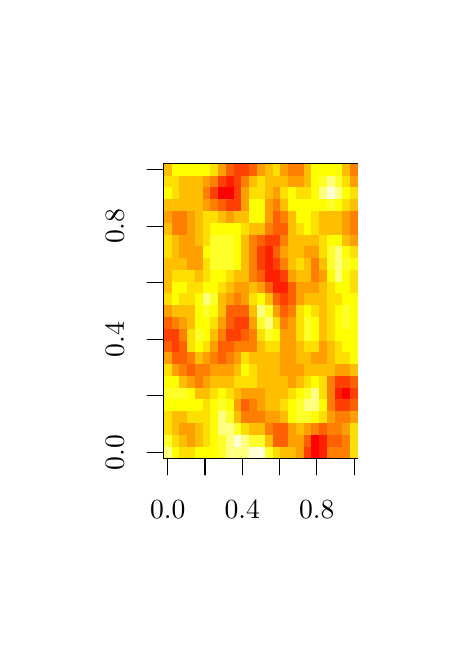
\begin{tikzpicture}[x=1pt,y=1pt]
\definecolor{fillColor}{RGB}{255,255,255}
\path[use as bounding box,fill=fillColor,fill opacity=0.00] (0,0) rectangle (144.54,216.81);
\begin{scope}
\path[clip] (  0.00,  0.00) rectangle (144.54,216.81);
\definecolor{drawColor}{RGB}{0,0,0}

\path[draw=drawColor,line width= 0.4pt,line join=round,line cap=round] ( 50.60, 61.20) -- (117.94, 61.20);

\path[draw=drawColor,line width= 0.4pt,line join=round,line cap=round] ( 50.60, 61.20) -- ( 50.60, 55.20);

\path[draw=drawColor,line width= 0.4pt,line join=round,line cap=round] ( 64.07, 61.20) -- ( 64.07, 55.20);

\path[draw=drawColor,line width= 0.4pt,line join=round,line cap=round] ( 77.54, 61.20) -- ( 77.54, 55.20);

\path[draw=drawColor,line width= 0.4pt,line join=round,line cap=round] ( 91.00, 61.20) -- ( 91.00, 55.20);

\path[draw=drawColor,line width= 0.4pt,line join=round,line cap=round] (104.47, 61.20) -- (104.47, 55.20);

\path[draw=drawColor,line width= 0.4pt,line join=round,line cap=round] (117.94, 61.20) -- (117.94, 55.20);

\node[text=drawColor,anchor=base,inner sep=0pt, outer sep=0pt, scale=  1.00] at ( 50.60, 39.60) {0.0};

\node[text=drawColor,anchor=base,inner sep=0pt, outer sep=0pt, scale=  1.00] at ( 77.54, 39.60) {0.4};

\node[text=drawColor,anchor=base,inner sep=0pt, outer sep=0pt, scale=  1.00] at (104.47, 39.60) {0.8};

\path[draw=drawColor,line width= 0.4pt,line join=round,line cap=round] ( 49.20, 63.33) -- ( 49.20,165.48);

\path[draw=drawColor,line width= 0.4pt,line join=round,line cap=round] ( 49.20, 63.33) -- ( 43.20, 63.33);

\path[draw=drawColor,line width= 0.4pt,line join=round,line cap=round] ( 49.20, 83.76) -- ( 43.20, 83.76);

\path[draw=drawColor,line width= 0.4pt,line join=round,line cap=round] ( 49.20,104.19) -- ( 43.20,104.19);

\path[draw=drawColor,line width= 0.4pt,line join=round,line cap=round] ( 49.20,124.62) -- ( 43.20,124.62);

\path[draw=drawColor,line width= 0.4pt,line join=round,line cap=round] ( 49.20,145.05) -- ( 43.20,145.05);

\path[draw=drawColor,line width= 0.4pt,line join=round,line cap=round] ( 49.20,165.48) -- ( 43.20,165.48);

\node[text=drawColor,rotate= 90.00,anchor=base,inner sep=0pt, outer sep=0pt, scale=  1.00] at ( 34.80, 63.33) {0.0};

\node[text=drawColor,rotate= 90.00,anchor=base,inner sep=0pt, outer sep=0pt, scale=  1.00] at ( 34.80,104.19) {0.4};

\node[text=drawColor,rotate= 90.00,anchor=base,inner sep=0pt, outer sep=0pt, scale=  1.00] at ( 34.80,145.05) {0.8};

\path[draw=drawColor,line width= 0.4pt,line join=round,line cap=round] ( 49.20, 61.20) --
	(119.34, 61.20) --
	(119.34,167.61) --
	( 49.20,167.61) --
	( 49.20, 61.20);
\end{scope}
\begin{scope}
\path[clip] ( 49.20, 61.20) rectangle (119.34,167.61);
\definecolor{fillColor}{RGB}{255,255,128}

\path[fill=fillColor] ( 49.20, 61.20) rectangle ( 52.01, 65.46);
\definecolor{fillColor}{RGB}{255,255,42}

\path[fill=fillColor] ( 49.20, 65.46) rectangle ( 52.01, 69.71);
\definecolor{fillColor}{RGB}{255,223,0}

\path[fill=fillColor] ( 49.20, 69.71) rectangle ( 52.01, 73.97);

\path[fill=fillColor] ( 49.20, 73.97) rectangle ( 52.01, 78.23);
\definecolor{fillColor}{RGB}{255,255,0}

\path[fill=fillColor] ( 49.20, 78.23) rectangle ( 52.01, 82.48);
\definecolor{fillColor}{RGB}{255,255,42}

\path[fill=fillColor] ( 49.20, 82.48) rectangle ( 52.01, 86.74);
\definecolor{fillColor}{RGB}{255,255,0}

\path[fill=fillColor] ( 49.20, 86.74) rectangle ( 52.01, 90.99);
\definecolor{fillColor}{RGB}{255,223,0}

\path[fill=fillColor] ( 49.20, 90.99) rectangle ( 52.01, 95.25);
\definecolor{fillColor}{RGB}{255,159,0}

\path[fill=fillColor] ( 49.20, 95.25) rectangle ( 52.01, 99.51);
\definecolor{fillColor}{RGB}{255,96,0}

\path[fill=fillColor] ( 49.20, 99.51) rectangle ( 52.01,103.76);
\definecolor{fillColor}{RGB}{255,64,0}

\path[fill=fillColor] ( 49.20,103.76) rectangle ( 52.01,108.02);
\definecolor{fillColor}{RGB}{255,96,0}

\path[fill=fillColor] ( 49.20,108.02) rectangle ( 52.01,112.28);
\definecolor{fillColor}{RGB}{255,159,0}

\path[fill=fillColor] ( 49.20,112.28) rectangle ( 52.01,116.53);
\definecolor{fillColor}{RGB}{255,223,0}

\path[fill=fillColor] ( 49.20,116.53) rectangle ( 52.01,120.79);
\definecolor{fillColor}{RGB}{255,191,0}

\path[fill=fillColor] ( 49.20,120.79) rectangle ( 52.01,125.05);

\path[fill=fillColor] ( 49.20,125.05) rectangle ( 52.01,129.30);

\path[fill=fillColor] ( 49.20,129.30) rectangle ( 52.01,133.56);
\definecolor{fillColor}{RGB}{255,223,0}

\path[fill=fillColor] ( 49.20,133.56) rectangle ( 52.01,137.82);

\path[fill=fillColor] ( 49.20,137.82) rectangle ( 52.01,142.07);
\definecolor{fillColor}{RGB}{255,191,0}

\path[fill=fillColor] ( 49.20,142.07) rectangle ( 52.01,146.33);
\definecolor{fillColor}{RGB}{255,159,0}

\path[fill=fillColor] ( 49.20,146.33) rectangle ( 52.01,150.58);
\definecolor{fillColor}{RGB}{255,191,0}

\path[fill=fillColor] ( 49.20,150.58) rectangle ( 52.01,154.84);
\definecolor{fillColor}{RGB}{255,255,0}

\path[fill=fillColor] ( 49.20,154.84) rectangle ( 52.01,159.10);
\definecolor{fillColor}{RGB}{255,223,0}

\path[fill=fillColor] ( 49.20,159.10) rectangle ( 52.01,163.35);
\definecolor{fillColor}{RGB}{255,191,0}

\path[fill=fillColor] ( 49.20,163.35) rectangle ( 52.01,167.61);
\definecolor{fillColor}{RGB}{255,255,0}

\path[fill=fillColor] ( 52.01, 61.20) rectangle ( 54.81, 65.46);
\definecolor{fillColor}{RGB}{255,223,0}

\path[fill=fillColor] ( 52.01, 65.46) rectangle ( 54.81, 69.71);
\definecolor{fillColor}{RGB}{255,191,0}

\path[fill=fillColor] ( 52.01, 69.71) rectangle ( 54.81, 73.97);

\path[fill=fillColor] ( 52.01, 73.97) rectangle ( 54.81, 78.23);
\definecolor{fillColor}{RGB}{255,255,0}

\path[fill=fillColor] ( 52.01, 78.23) rectangle ( 54.81, 82.48);
\definecolor{fillColor}{RGB}{255,255,42}

\path[fill=fillColor] ( 52.01, 82.48) rectangle ( 54.81, 86.74);
\definecolor{fillColor}{RGB}{255,255,0}

\path[fill=fillColor] ( 52.01, 86.74) rectangle ( 54.81, 90.99);
\definecolor{fillColor}{RGB}{255,159,0}

\path[fill=fillColor] ( 52.01, 90.99) rectangle ( 54.81, 95.25);
\definecolor{fillColor}{RGB}{255,96,0}

\path[fill=fillColor] ( 52.01, 95.25) rectangle ( 54.81, 99.51);
\definecolor{fillColor}{RGB}{255,64,0}

\path[fill=fillColor] ( 52.01, 99.51) rectangle ( 54.81,103.76);

\path[fill=fillColor] ( 52.01,103.76) rectangle ( 54.81,108.02);
\definecolor{fillColor}{RGB}{255,128,0}

\path[fill=fillColor] ( 52.01,108.02) rectangle ( 54.81,112.28);
\definecolor{fillColor}{RGB}{255,191,0}

\path[fill=fillColor] ( 52.01,112.28) rectangle ( 54.81,116.53);
\definecolor{fillColor}{RGB}{255,255,0}

\path[fill=fillColor] ( 52.01,116.53) rectangle ( 54.81,120.79);

\path[fill=fillColor] ( 52.01,120.79) rectangle ( 54.81,125.05);
\definecolor{fillColor}{RGB}{255,223,0}

\path[fill=fillColor] ( 52.01,125.05) rectangle ( 54.81,129.30);
\definecolor{fillColor}{RGB}{255,191,0}

\path[fill=fillColor] ( 52.01,129.30) rectangle ( 54.81,133.56);

\path[fill=fillColor] ( 52.01,133.56) rectangle ( 54.81,137.82);

\path[fill=fillColor] ( 52.01,137.82) rectangle ( 54.81,142.07);
\definecolor{fillColor}{RGB}{255,128,0}

\path[fill=fillColor] ( 52.01,142.07) rectangle ( 54.81,146.33);

\path[fill=fillColor] ( 52.01,146.33) rectangle ( 54.81,150.58);
\definecolor{fillColor}{RGB}{255,191,0}

\path[fill=fillColor] ( 52.01,150.58) rectangle ( 54.81,154.84);
\definecolor{fillColor}{RGB}{255,223,0}

\path[fill=fillColor] ( 52.01,154.84) rectangle ( 54.81,159.10);

\path[fill=fillColor] ( 52.01,159.10) rectangle ( 54.81,163.35);
\definecolor{fillColor}{RGB}{255,255,0}

\path[fill=fillColor] ( 52.01,163.35) rectangle ( 54.81,167.61);
\definecolor{fillColor}{RGB}{255,223,0}

\path[fill=fillColor] ( 54.81, 61.20) rectangle ( 57.62, 65.46);
\definecolor{fillColor}{RGB}{255,191,0}

\path[fill=fillColor] ( 54.81, 65.46) rectangle ( 57.62, 69.71);
\definecolor{fillColor}{RGB}{255,159,0}

\path[fill=fillColor] ( 54.81, 69.71) rectangle ( 57.62, 73.97);
\definecolor{fillColor}{RGB}{255,191,0}

\path[fill=fillColor] ( 54.81, 73.97) rectangle ( 57.62, 78.23);
\definecolor{fillColor}{RGB}{255,255,0}

\path[fill=fillColor] ( 54.81, 78.23) rectangle ( 57.62, 82.48);
\definecolor{fillColor}{RGB}{255,255,42}

\path[fill=fillColor] ( 54.81, 82.48) rectangle ( 57.62, 86.74);
\definecolor{fillColor}{RGB}{255,191,0}

\path[fill=fillColor] ( 54.81, 86.74) rectangle ( 57.62, 90.99);
\definecolor{fillColor}{RGB}{255,128,0}

\path[fill=fillColor] ( 54.81, 90.99) rectangle ( 57.62, 95.25);
\definecolor{fillColor}{RGB}{255,96,0}

\path[fill=fillColor] ( 54.81, 95.25) rectangle ( 57.62, 99.51);

\path[fill=fillColor] ( 54.81, 99.51) rectangle ( 57.62,103.76);
\definecolor{fillColor}{RGB}{255,128,0}

\path[fill=fillColor] ( 54.81,103.76) rectangle ( 57.62,108.02);
\definecolor{fillColor}{RGB}{255,159,0}

\path[fill=fillColor] ( 54.81,108.02) rectangle ( 57.62,112.28);
\definecolor{fillColor}{RGB}{255,191,0}

\path[fill=fillColor] ( 54.81,112.28) rectangle ( 57.62,116.53);
\definecolor{fillColor}{RGB}{255,223,0}

\path[fill=fillColor] ( 54.81,116.53) rectangle ( 57.62,120.79);
\definecolor{fillColor}{RGB}{255,255,0}

\path[fill=fillColor] ( 54.81,120.79) rectangle ( 57.62,125.05);
\definecolor{fillColor}{RGB}{255,223,0}

\path[fill=fillColor] ( 54.81,125.05) rectangle ( 57.62,129.30);
\definecolor{fillColor}{RGB}{255,191,0}

\path[fill=fillColor] ( 54.81,129.30) rectangle ( 57.62,133.56);
\definecolor{fillColor}{RGB}{255,159,0}

\path[fill=fillColor] ( 54.81,133.56) rectangle ( 57.62,137.82);

\path[fill=fillColor] ( 54.81,137.82) rectangle ( 57.62,142.07);
\definecolor{fillColor}{RGB}{255,128,0}

\path[fill=fillColor] ( 54.81,142.07) rectangle ( 57.62,146.33);

\path[fill=fillColor] ( 54.81,146.33) rectangle ( 57.62,150.58);
\definecolor{fillColor}{RGB}{255,191,0}

\path[fill=fillColor] ( 54.81,150.58) rectangle ( 57.62,154.84);

\path[fill=fillColor] ( 54.81,154.84) rectangle ( 57.62,159.10);

\path[fill=fillColor] ( 54.81,159.10) rectangle ( 57.62,163.35);
\definecolor{fillColor}{RGB}{255,255,0}

\path[fill=fillColor] ( 54.81,163.35) rectangle ( 57.62,167.61);
\definecolor{fillColor}{RGB}{255,223,0}

\path[fill=fillColor] ( 57.62, 61.20) rectangle ( 60.42, 65.46);
\definecolor{fillColor}{RGB}{255,159,0}

\path[fill=fillColor] ( 57.62, 65.46) rectangle ( 60.42, 69.71);

\path[fill=fillColor] ( 57.62, 69.71) rectangle ( 60.42, 73.97);
\definecolor{fillColor}{RGB}{255,223,0}

\path[fill=fillColor] ( 57.62, 73.97) rectangle ( 60.42, 78.23);
\definecolor{fillColor}{RGB}{255,255,0}

\path[fill=fillColor] ( 57.62, 78.23) rectangle ( 60.42, 82.48);

\path[fill=fillColor] ( 57.62, 82.48) rectangle ( 60.42, 86.74);
\definecolor{fillColor}{RGB}{255,159,0}

\path[fill=fillColor] ( 57.62, 86.74) rectangle ( 60.42, 90.99);
\definecolor{fillColor}{RGB}{255,96,0}

\path[fill=fillColor] ( 57.62, 90.99) rectangle ( 60.42, 95.25);
\definecolor{fillColor}{RGB}{255,128,0}

\path[fill=fillColor] ( 57.62, 95.25) rectangle ( 60.42, 99.51);
\definecolor{fillColor}{RGB}{255,223,0}

\path[fill=fillColor] ( 57.62, 99.51) rectangle ( 60.42,103.76);

\path[fill=fillColor] ( 57.62,103.76) rectangle ( 60.42,108.02);
\definecolor{fillColor}{RGB}{255,191,0}

\path[fill=fillColor] ( 57.62,108.02) rectangle ( 60.42,112.28);

\path[fill=fillColor] ( 57.62,112.28) rectangle ( 60.42,116.53);
\definecolor{fillColor}{RGB}{255,223,0}

\path[fill=fillColor] ( 57.62,116.53) rectangle ( 60.42,120.79);

\path[fill=fillColor] ( 57.62,120.79) rectangle ( 60.42,125.05);

\path[fill=fillColor] ( 57.62,125.05) rectangle ( 60.42,129.30);
\definecolor{fillColor}{RGB}{255,159,0}

\path[fill=fillColor] ( 57.62,129.30) rectangle ( 60.42,133.56);

\path[fill=fillColor] ( 57.62,133.56) rectangle ( 60.42,137.82);

\path[fill=fillColor] ( 57.62,137.82) rectangle ( 60.42,142.07);

\path[fill=fillColor] ( 57.62,142.07) rectangle ( 60.42,146.33);

\path[fill=fillColor] ( 57.62,146.33) rectangle ( 60.42,150.58);
\definecolor{fillColor}{RGB}{255,191,0}

\path[fill=fillColor] ( 57.62,150.58) rectangle ( 60.42,154.84);

\path[fill=fillColor] ( 57.62,154.84) rectangle ( 60.42,159.10);

\path[fill=fillColor] ( 57.62,159.10) rectangle ( 60.42,163.35);
\definecolor{fillColor}{RGB}{255,255,0}

\path[fill=fillColor] ( 57.62,163.35) rectangle ( 60.42,167.61);

\path[fill=fillColor] ( 60.42, 61.20) rectangle ( 63.23, 65.46);
\definecolor{fillColor}{RGB}{255,191,0}

\path[fill=fillColor] ( 60.42, 65.46) rectangle ( 63.23, 69.71);

\path[fill=fillColor] ( 60.42, 69.71) rectangle ( 63.23, 73.97);
\definecolor{fillColor}{RGB}{255,223,0}

\path[fill=fillColor] ( 60.42, 73.97) rectangle ( 63.23, 78.23);
\definecolor{fillColor}{RGB}{255,255,0}

\path[fill=fillColor] ( 60.42, 78.23) rectangle ( 63.23, 82.48);
\definecolor{fillColor}{RGB}{255,191,0}

\path[fill=fillColor] ( 60.42, 82.48) rectangle ( 63.23, 86.74);
\definecolor{fillColor}{RGB}{255,128,0}

\path[fill=fillColor] ( 60.42, 86.74) rectangle ( 63.23, 90.99);

\path[fill=fillColor] ( 60.42, 90.99) rectangle ( 63.23, 95.25);
\definecolor{fillColor}{RGB}{255,191,0}

\path[fill=fillColor] ( 60.42, 95.25) rectangle ( 63.23, 99.51);
\definecolor{fillColor}{RGB}{255,255,0}

\path[fill=fillColor] ( 60.42, 99.51) rectangle ( 63.23,103.76);
\definecolor{fillColor}{RGB}{255,255,42}

\path[fill=fillColor] ( 60.42,103.76) rectangle ( 63.23,108.02);
\definecolor{fillColor}{RGB}{255,255,0}

\path[fill=fillColor] ( 60.42,108.02) rectangle ( 63.23,112.28);

\path[fill=fillColor] ( 60.42,112.28) rectangle ( 63.23,116.53);

\path[fill=fillColor] ( 60.42,116.53) rectangle ( 63.23,120.79);
\definecolor{fillColor}{RGB}{255,223,0}

\path[fill=fillColor] ( 60.42,120.79) rectangle ( 63.23,125.05);
\definecolor{fillColor}{RGB}{255,191,0}

\path[fill=fillColor] ( 60.42,125.05) rectangle ( 63.23,129.30);
\definecolor{fillColor}{RGB}{255,159,0}

\path[fill=fillColor] ( 60.42,129.30) rectangle ( 63.23,133.56);

\path[fill=fillColor] ( 60.42,133.56) rectangle ( 63.23,137.82);
\definecolor{fillColor}{RGB}{255,191,0}

\path[fill=fillColor] ( 60.42,137.82) rectangle ( 63.23,142.07);

\path[fill=fillColor] ( 60.42,142.07) rectangle ( 63.23,146.33);

\path[fill=fillColor] ( 60.42,146.33) rectangle ( 63.23,150.58);

\path[fill=fillColor] ( 60.42,150.58) rectangle ( 63.23,154.84);

\path[fill=fillColor] ( 60.42,154.84) rectangle ( 63.23,159.10);

\path[fill=fillColor] ( 60.42,159.10) rectangle ( 63.23,163.35);
\definecolor{fillColor}{RGB}{255,255,0}

\path[fill=fillColor] ( 60.42,163.35) rectangle ( 63.23,167.61);

\path[fill=fillColor] ( 63.23, 61.20) rectangle ( 66.03, 65.46);
\definecolor{fillColor}{RGB}{255,223,0}

\path[fill=fillColor] ( 63.23, 65.46) rectangle ( 66.03, 69.71);

\path[fill=fillColor] ( 63.23, 69.71) rectangle ( 66.03, 73.97);

\path[fill=fillColor] ( 63.23, 73.97) rectangle ( 66.03, 78.23);

\path[fill=fillColor] ( 63.23, 78.23) rectangle ( 66.03, 82.48);
\definecolor{fillColor}{RGB}{255,191,0}

\path[fill=fillColor] ( 63.23, 82.48) rectangle ( 66.03, 86.74);
\definecolor{fillColor}{RGB}{255,159,0}

\path[fill=fillColor] ( 63.23, 86.74) rectangle ( 66.03, 90.99);
\definecolor{fillColor}{RGB}{255,128,0}

\path[fill=fillColor] ( 63.23, 90.99) rectangle ( 66.03, 95.25);
\definecolor{fillColor}{RGB}{255,159,0}

\path[fill=fillColor] ( 63.23, 95.25) rectangle ( 66.03, 99.51);
\definecolor{fillColor}{RGB}{255,223,0}

\path[fill=fillColor] ( 63.23, 99.51) rectangle ( 66.03,103.76);
\definecolor{fillColor}{RGB}{255,255,0}

\path[fill=fillColor] ( 63.23,103.76) rectangle ( 66.03,108.02);

\path[fill=fillColor] ( 63.23,108.02) rectangle ( 66.03,112.28);
\definecolor{fillColor}{RGB}{255,255,42}

\path[fill=fillColor] ( 63.23,112.28) rectangle ( 66.03,116.53);
\definecolor{fillColor}{RGB}{255,255,128}

\path[fill=fillColor] ( 63.23,116.53) rectangle ( 66.03,120.79);
\definecolor{fillColor}{RGB}{255,255,0}

\path[fill=fillColor] ( 63.23,120.79) rectangle ( 66.03,125.05);
\definecolor{fillColor}{RGB}{255,223,0}

\path[fill=fillColor] ( 63.23,125.05) rectangle ( 66.03,129.30);

\path[fill=fillColor] ( 63.23,129.30) rectangle ( 66.03,133.56);
\definecolor{fillColor}{RGB}{255,255,0}

\path[fill=fillColor] ( 63.23,133.56) rectangle ( 66.03,137.82);
\definecolor{fillColor}{RGB}{255,223,0}

\path[fill=fillColor] ( 63.23,137.82) rectangle ( 66.03,142.07);

\path[fill=fillColor] ( 63.23,142.07) rectangle ( 66.03,146.33);

\path[fill=fillColor] ( 63.23,146.33) rectangle ( 66.03,150.58);
\definecolor{fillColor}{RGB}{255,159,0}

\path[fill=fillColor] ( 63.23,150.58) rectangle ( 66.03,154.84);
\definecolor{fillColor}{RGB}{255,128,0}

\path[fill=fillColor] ( 63.23,154.84) rectangle ( 66.03,159.10);
\definecolor{fillColor}{RGB}{255,159,0}

\path[fill=fillColor] ( 63.23,159.10) rectangle ( 66.03,163.35);
\definecolor{fillColor}{RGB}{255,255,0}

\path[fill=fillColor] ( 63.23,163.35) rectangle ( 66.03,167.61);

\path[fill=fillColor] ( 66.03, 61.20) rectangle ( 68.84, 65.46);

\path[fill=fillColor] ( 66.03, 65.46) rectangle ( 68.84, 69.71);

\path[fill=fillColor] ( 66.03, 69.71) rectangle ( 68.84, 73.97);

\path[fill=fillColor] ( 66.03, 73.97) rectangle ( 68.84, 78.23);

\path[fill=fillColor] ( 66.03, 78.23) rectangle ( 68.84, 82.48);
\definecolor{fillColor}{RGB}{255,223,0}

\path[fill=fillColor] ( 66.03, 82.48) rectangle ( 68.84, 86.74);
\definecolor{fillColor}{RGB}{255,191,0}

\path[fill=fillColor] ( 66.03, 86.74) rectangle ( 68.84, 90.99);
\definecolor{fillColor}{RGB}{255,159,0}

\path[fill=fillColor] ( 66.03, 90.99) rectangle ( 68.84, 95.25);
\definecolor{fillColor}{RGB}{255,128,0}

\path[fill=fillColor] ( 66.03, 95.25) rectangle ( 68.84, 99.51);
\definecolor{fillColor}{RGB}{255,159,0}

\path[fill=fillColor] ( 66.03, 99.51) rectangle ( 68.84,103.76);
\definecolor{fillColor}{RGB}{255,191,0}

\path[fill=fillColor] ( 66.03,103.76) rectangle ( 68.84,108.02);
\definecolor{fillColor}{RGB}{255,223,0}

\path[fill=fillColor] ( 66.03,108.02) rectangle ( 68.84,112.28);
\definecolor{fillColor}{RGB}{255,255,0}

\path[fill=fillColor] ( 66.03,112.28) rectangle ( 68.84,116.53);
\definecolor{fillColor}{RGB}{255,255,42}

\path[fill=fillColor] ( 66.03,116.53) rectangle ( 68.84,120.79);
\definecolor{fillColor}{RGB}{255,255,0}

\path[fill=fillColor] ( 66.03,120.79) rectangle ( 68.84,125.05);

\path[fill=fillColor] ( 66.03,125.05) rectangle ( 68.84,129.30);
\definecolor{fillColor}{RGB}{255,255,42}

\path[fill=fillColor] ( 66.03,129.30) rectangle ( 68.84,133.56);

\path[fill=fillColor] ( 66.03,133.56) rectangle ( 68.84,137.82);

\path[fill=fillColor] ( 66.03,137.82) rectangle ( 68.84,142.07);
\definecolor{fillColor}{RGB}{255,255,0}

\path[fill=fillColor] ( 66.03,142.07) rectangle ( 68.84,146.33);
\definecolor{fillColor}{RGB}{255,223,0}

\path[fill=fillColor] ( 66.03,146.33) rectangle ( 68.84,150.58);
\definecolor{fillColor}{RGB}{255,128,0}

\path[fill=fillColor] ( 66.03,150.58) rectangle ( 68.84,154.84);
\definecolor{fillColor}{RGB}{255,64,0}

\path[fill=fillColor] ( 66.03,154.84) rectangle ( 68.84,159.10);
\definecolor{fillColor}{RGB}{255,128,0}

\path[fill=fillColor] ( 66.03,159.10) rectangle ( 68.84,163.35);
\definecolor{fillColor}{RGB}{255,223,0}

\path[fill=fillColor] ( 66.03,163.35) rectangle ( 68.84,167.61);
\definecolor{fillColor}{RGB}{255,255,42}

\path[fill=fillColor] ( 68.84, 61.20) rectangle ( 71.64, 65.46);

\path[fill=fillColor] ( 68.84, 65.46) rectangle ( 71.64, 69.71);
\definecolor{fillColor}{RGB}{255,255,128}

\path[fill=fillColor] ( 68.84, 69.71) rectangle ( 71.64, 73.97);

\path[fill=fillColor] ( 68.84, 73.97) rectangle ( 71.64, 78.23);
\definecolor{fillColor}{RGB}{255,255,42}

\path[fill=fillColor] ( 68.84, 78.23) rectangle ( 71.64, 82.48);
\definecolor{fillColor}{RGB}{255,255,0}

\path[fill=fillColor] ( 68.84, 82.48) rectangle ( 71.64, 86.74);
\definecolor{fillColor}{RGB}{255,191,0}

\path[fill=fillColor] ( 68.84, 86.74) rectangle ( 71.64, 90.99);
\definecolor{fillColor}{RGB}{255,159,0}

\path[fill=fillColor] ( 68.84, 90.99) rectangle ( 71.64, 95.25);
\definecolor{fillColor}{RGB}{255,96,0}

\path[fill=fillColor] ( 68.84, 95.25) rectangle ( 71.64, 99.51);

\path[fill=fillColor] ( 68.84, 99.51) rectangle ( 71.64,103.76);
\definecolor{fillColor}{RGB}{255,128,0}

\path[fill=fillColor] ( 68.84,103.76) rectangle ( 71.64,108.02);
\definecolor{fillColor}{RGB}{255,159,0}

\path[fill=fillColor] ( 68.84,108.02) rectangle ( 71.64,112.28);
\definecolor{fillColor}{RGB}{255,191,0}

\path[fill=fillColor] ( 68.84,112.28) rectangle ( 71.64,116.53);

\path[fill=fillColor] ( 68.84,116.53) rectangle ( 71.64,120.79);
\definecolor{fillColor}{RGB}{255,223,0}

\path[fill=fillColor] ( 68.84,120.79) rectangle ( 71.64,125.05);
\definecolor{fillColor}{RGB}{255,255,0}

\path[fill=fillColor] ( 68.84,125.05) rectangle ( 71.64,129.30);
\definecolor{fillColor}{RGB}{255,255,42}

\path[fill=fillColor] ( 68.84,129.30) rectangle ( 71.64,133.56);

\path[fill=fillColor] ( 68.84,133.56) rectangle ( 71.64,137.82);

\path[fill=fillColor] ( 68.84,137.82) rectangle ( 71.64,142.07);
\definecolor{fillColor}{RGB}{255,255,0}

\path[fill=fillColor] ( 68.84,142.07) rectangle ( 71.64,146.33);
\definecolor{fillColor}{RGB}{255,191,0}

\path[fill=fillColor] ( 68.84,146.33) rectangle ( 71.64,150.58);
\definecolor{fillColor}{RGB}{255,96,0}

\path[fill=fillColor] ( 68.84,150.58) rectangle ( 71.64,154.84);
\definecolor{fillColor}{RGB}{255,0,0}

\path[fill=fillColor] ( 68.84,154.84) rectangle ( 71.64,159.10);
\definecolor{fillColor}{RGB}{255,64,0}

\path[fill=fillColor] ( 68.84,159.10) rectangle ( 71.64,163.35);
\definecolor{fillColor}{RGB}{255,159,0}

\path[fill=fillColor] ( 68.84,163.35) rectangle ( 71.64,167.61);
\definecolor{fillColor}{RGB}{255,255,128}

\path[fill=fillColor] ( 71.64, 61.20) rectangle ( 74.45, 65.46);

\path[fill=fillColor] ( 71.64, 65.46) rectangle ( 74.45, 69.71);

\path[fill=fillColor] ( 71.64, 69.71) rectangle ( 74.45, 73.97);
\definecolor{fillColor}{RGB}{255,255,42}

\path[fill=fillColor] ( 71.64, 73.97) rectangle ( 74.45, 78.23);
\definecolor{fillColor}{RGB}{255,255,0}

\path[fill=fillColor] ( 71.64, 78.23) rectangle ( 74.45, 82.48);
\definecolor{fillColor}{RGB}{255,223,0}

\path[fill=fillColor] ( 71.64, 82.48) rectangle ( 74.45, 86.74);
\definecolor{fillColor}{RGB}{255,191,0}

\path[fill=fillColor] ( 71.64, 86.74) rectangle ( 74.45, 90.99);
\definecolor{fillColor}{RGB}{255,159,0}

\path[fill=fillColor] ( 71.64, 90.99) rectangle ( 74.45, 95.25);
\definecolor{fillColor}{RGB}{255,128,0}

\path[fill=fillColor] ( 71.64, 95.25) rectangle ( 74.45, 99.51);
\definecolor{fillColor}{RGB}{255,96,0}

\path[fill=fillColor] ( 71.64, 99.51) rectangle ( 74.45,103.76);
\definecolor{fillColor}{RGB}{255,64,0}

\path[fill=fillColor] ( 71.64,103.76) rectangle ( 74.45,108.02);
\definecolor{fillColor}{RGB}{255,96,0}

\path[fill=fillColor] ( 71.64,108.02) rectangle ( 74.45,112.28);

\path[fill=fillColor] ( 71.64,112.28) rectangle ( 74.45,116.53);
\definecolor{fillColor}{RGB}{255,159,0}

\path[fill=fillColor] ( 71.64,116.53) rectangle ( 74.45,120.79);
\definecolor{fillColor}{RGB}{255,191,0}

\path[fill=fillColor] ( 71.64,120.79) rectangle ( 74.45,125.05);
\definecolor{fillColor}{RGB}{255,223,0}

\path[fill=fillColor] ( 71.64,125.05) rectangle ( 74.45,129.30);
\definecolor{fillColor}{RGB}{255,255,42}

\path[fill=fillColor] ( 71.64,129.30) rectangle ( 74.45,133.56);

\path[fill=fillColor] ( 71.64,133.56) rectangle ( 74.45,137.82);

\path[fill=fillColor] ( 71.64,137.82) rectangle ( 74.45,142.07);
\definecolor{fillColor}{RGB}{255,255,0}

\path[fill=fillColor] ( 71.64,142.07) rectangle ( 74.45,146.33);
\definecolor{fillColor}{RGB}{255,159,0}

\path[fill=fillColor] ( 71.64,146.33) rectangle ( 74.45,150.58);
\definecolor{fillColor}{RGB}{255,64,0}

\path[fill=fillColor] ( 71.64,150.58) rectangle ( 74.45,154.84);
\definecolor{fillColor}{RGB}{255,0,0}

\path[fill=fillColor] ( 71.64,154.84) rectangle ( 74.45,159.10);
\definecolor{fillColor}{RGB}{255,32,0}

\path[fill=fillColor] ( 71.64,159.10) rectangle ( 74.45,163.35);
\definecolor{fillColor}{RGB}{255,96,0}

\path[fill=fillColor] ( 71.64,163.35) rectangle ( 74.45,167.61);
\definecolor{fillColor}{RGB}{255,255,128}

\path[fill=fillColor] ( 74.45, 61.20) rectangle ( 77.26, 65.46);
\definecolor{fillColor}{RGB}{255,255,213}

\path[fill=fillColor] ( 74.45, 65.46) rectangle ( 77.26, 69.71);
\definecolor{fillColor}{RGB}{255,255,42}

\path[fill=fillColor] ( 74.45, 69.71) rectangle ( 77.26, 73.97);
\definecolor{fillColor}{RGB}{255,191,0}

\path[fill=fillColor] ( 74.45, 73.97) rectangle ( 77.26, 78.23);
\definecolor{fillColor}{RGB}{255,159,0}

\path[fill=fillColor] ( 74.45, 78.23) rectangle ( 77.26, 82.48);
\definecolor{fillColor}{RGB}{255,191,0}

\path[fill=fillColor] ( 74.45, 82.48) rectangle ( 77.26, 86.74);
\definecolor{fillColor}{RGB}{255,223,0}

\path[fill=fillColor] ( 74.45, 86.74) rectangle ( 77.26, 90.99);
\definecolor{fillColor}{RGB}{255,191,0}

\path[fill=fillColor] ( 74.45, 90.99) rectangle ( 77.26, 95.25);
\definecolor{fillColor}{RGB}{255,159,0}

\path[fill=fillColor] ( 74.45, 95.25) rectangle ( 77.26, 99.51);
\definecolor{fillColor}{RGB}{255,128,0}

\path[fill=fillColor] ( 74.45, 99.51) rectangle ( 77.26,103.76);
\definecolor{fillColor}{RGB}{255,64,0}

\path[fill=fillColor] ( 74.45,103.76) rectangle ( 77.26,108.02);

\path[fill=fillColor] ( 74.45,108.02) rectangle ( 77.26,112.28);
\definecolor{fillColor}{RGB}{255,96,0}

\path[fill=fillColor] ( 74.45,112.28) rectangle ( 77.26,116.53);
\definecolor{fillColor}{RGB}{255,128,0}

\path[fill=fillColor] ( 74.45,116.53) rectangle ( 77.26,120.79);
\definecolor{fillColor}{RGB}{255,159,0}

\path[fill=fillColor] ( 74.45,120.79) rectangle ( 77.26,125.05);
\definecolor{fillColor}{RGB}{255,191,0}

\path[fill=fillColor] ( 74.45,125.05) rectangle ( 77.26,129.30);
\definecolor{fillColor}{RGB}{255,255,0}

\path[fill=fillColor] ( 74.45,129.30) rectangle ( 77.26,133.56);

\path[fill=fillColor] ( 74.45,133.56) rectangle ( 77.26,137.82);

\path[fill=fillColor] ( 74.45,137.82) rectangle ( 77.26,142.07);

\path[fill=fillColor] ( 74.45,142.07) rectangle ( 77.26,146.33);
\definecolor{fillColor}{RGB}{255,191,0}

\path[fill=fillColor] ( 74.45,146.33) rectangle ( 77.26,150.58);
\definecolor{fillColor}{RGB}{255,64,0}

\path[fill=fillColor] ( 74.45,150.58) rectangle ( 77.26,154.84);

\path[fill=fillColor] ( 74.45,154.84) rectangle ( 77.26,159.10);

\path[fill=fillColor] ( 74.45,159.10) rectangle ( 77.26,163.35);

\path[fill=fillColor] ( 74.45,163.35) rectangle ( 77.26,167.61);
\definecolor{fillColor}{RGB}{255,255,128}

\path[fill=fillColor] ( 77.26, 61.20) rectangle ( 80.06, 65.46);

\path[fill=fillColor] ( 77.26, 65.46) rectangle ( 80.06, 69.71);
\definecolor{fillColor}{RGB}{255,223,0}

\path[fill=fillColor] ( 77.26, 69.71) rectangle ( 80.06, 73.97);
\definecolor{fillColor}{RGB}{255,128,0}

\path[fill=fillColor] ( 77.26, 73.97) rectangle ( 80.06, 78.23);
\definecolor{fillColor}{RGB}{255,96,0}

\path[fill=fillColor] ( 77.26, 78.23) rectangle ( 80.06, 82.48);
\definecolor{fillColor}{RGB}{255,159,0}

\path[fill=fillColor] ( 77.26, 82.48) rectangle ( 80.06, 86.74);
\definecolor{fillColor}{RGB}{255,223,0}

\path[fill=fillColor] ( 77.26, 86.74) rectangle ( 80.06, 90.99);
\definecolor{fillColor}{RGB}{255,255,0}

\path[fill=fillColor] ( 77.26, 90.99) rectangle ( 80.06, 95.25);
\definecolor{fillColor}{RGB}{255,223,0}

\path[fill=fillColor] ( 77.26, 95.25) rectangle ( 80.06, 99.51);
\definecolor{fillColor}{RGB}{255,128,0}

\path[fill=fillColor] ( 77.26, 99.51) rectangle ( 80.06,103.76);
\definecolor{fillColor}{RGB}{255,96,0}

\path[fill=fillColor] ( 77.26,103.76) rectangle ( 80.06,108.02);
\definecolor{fillColor}{RGB}{255,64,0}

\path[fill=fillColor] ( 77.26,108.02) rectangle ( 80.06,112.28);
\definecolor{fillColor}{RGB}{255,96,0}

\path[fill=fillColor] ( 77.26,112.28) rectangle ( 80.06,116.53);
\definecolor{fillColor}{RGB}{255,159,0}

\path[fill=fillColor] ( 77.26,116.53) rectangle ( 80.06,120.79);

\path[fill=fillColor] ( 77.26,120.79) rectangle ( 80.06,125.05);
\definecolor{fillColor}{RGB}{255,191,0}

\path[fill=fillColor] ( 77.26,125.05) rectangle ( 80.06,129.30);

\path[fill=fillColor] ( 77.26,129.30) rectangle ( 80.06,133.56);

\path[fill=fillColor] ( 77.26,133.56) rectangle ( 80.06,137.82);

\path[fill=fillColor] ( 77.26,137.82) rectangle ( 80.06,142.07);
\definecolor{fillColor}{RGB}{255,223,0}

\path[fill=fillColor] ( 77.26,142.07) rectangle ( 80.06,146.33);
\definecolor{fillColor}{RGB}{255,191,0}

\path[fill=fillColor] ( 77.26,146.33) rectangle ( 80.06,150.58);
\definecolor{fillColor}{RGB}{255,159,0}

\path[fill=fillColor] ( 77.26,150.58) rectangle ( 80.06,154.84);

\path[fill=fillColor] ( 77.26,154.84) rectangle ( 80.06,159.10);
\definecolor{fillColor}{RGB}{255,128,0}

\path[fill=fillColor] ( 77.26,159.10) rectangle ( 80.06,163.35);
\definecolor{fillColor}{RGB}{255,64,0}

\path[fill=fillColor] ( 77.26,163.35) rectangle ( 80.06,167.61);
\definecolor{fillColor}{RGB}{255,255,213}

\path[fill=fillColor] ( 80.06, 61.20) rectangle ( 82.87, 65.46);
\definecolor{fillColor}{RGB}{255,255,42}

\path[fill=fillColor] ( 80.06, 65.46) rectangle ( 82.87, 69.71);
\definecolor{fillColor}{RGB}{255,191,0}

\path[fill=fillColor] ( 80.06, 69.71) rectangle ( 82.87, 73.97);
\definecolor{fillColor}{RGB}{255,128,0}

\path[fill=fillColor] ( 80.06, 73.97) rectangle ( 82.87, 78.23);

\path[fill=fillColor] ( 80.06, 78.23) rectangle ( 82.87, 82.48);
\definecolor{fillColor}{RGB}{255,159,0}

\path[fill=fillColor] ( 80.06, 82.48) rectangle ( 82.87, 86.74);
\definecolor{fillColor}{RGB}{255,223,0}

\path[fill=fillColor] ( 80.06, 86.74) rectangle ( 82.87, 90.99);

\path[fill=fillColor] ( 80.06, 90.99) rectangle ( 82.87, 95.25);
\definecolor{fillColor}{RGB}{255,191,0}

\path[fill=fillColor] ( 80.06, 95.25) rectangle ( 82.87, 99.51);
\definecolor{fillColor}{RGB}{255,128,0}

\path[fill=fillColor] ( 80.06, 99.51) rectangle ( 82.87,103.76);

\path[fill=fillColor] ( 80.06,103.76) rectangle ( 82.87,108.02);
\definecolor{fillColor}{RGB}{255,159,0}

\path[fill=fillColor] ( 80.06,108.02) rectangle ( 82.87,112.28);
\definecolor{fillColor}{RGB}{255,191,0}

\path[fill=fillColor] ( 80.06,112.28) rectangle ( 82.87,116.53);
\definecolor{fillColor}{RGB}{255,223,0}

\path[fill=fillColor] ( 80.06,116.53) rectangle ( 82.87,120.79);
\definecolor{fillColor}{RGB}{255,191,0}

\path[fill=fillColor] ( 80.06,120.79) rectangle ( 82.87,125.05);
\definecolor{fillColor}{RGB}{255,128,0}

\path[fill=fillColor] ( 80.06,125.05) rectangle ( 82.87,129.30);

\path[fill=fillColor] ( 80.06,129.30) rectangle ( 82.87,133.56);

\path[fill=fillColor] ( 80.06,133.56) rectangle ( 82.87,137.82);

\path[fill=fillColor] ( 80.06,137.82) rectangle ( 82.87,142.07);
\definecolor{fillColor}{RGB}{255,191,0}

\path[fill=fillColor] ( 80.06,142.07) rectangle ( 82.87,146.33);
\definecolor{fillColor}{RGB}{255,255,0}

\path[fill=fillColor] ( 80.06,146.33) rectangle ( 82.87,150.58);

\path[fill=fillColor] ( 80.06,150.58) rectangle ( 82.87,154.84);
\definecolor{fillColor}{RGB}{255,223,0}

\path[fill=fillColor] ( 80.06,154.84) rectangle ( 82.87,159.10);
\definecolor{fillColor}{RGB}{255,191,0}

\path[fill=fillColor] ( 80.06,159.10) rectangle ( 82.87,163.35);
\definecolor{fillColor}{RGB}{255,96,0}

\path[fill=fillColor] ( 80.06,163.35) rectangle ( 82.87,167.61);
\definecolor{fillColor}{RGB}{255,255,213}

\path[fill=fillColor] ( 82.87, 61.20) rectangle ( 85.67, 65.46);
\definecolor{fillColor}{RGB}{255,255,42}

\path[fill=fillColor] ( 82.87, 65.46) rectangle ( 85.67, 69.71);
\definecolor{fillColor}{RGB}{255,191,0}

\path[fill=fillColor] ( 82.87, 69.71) rectangle ( 85.67, 73.97);
\definecolor{fillColor}{RGB}{255,128,0}

\path[fill=fillColor] ( 82.87, 73.97) rectangle ( 85.67, 78.23);
\definecolor{fillColor}{RGB}{255,159,0}

\path[fill=fillColor] ( 82.87, 78.23) rectangle ( 85.67, 82.48);

\path[fill=fillColor] ( 82.87, 82.48) rectangle ( 85.67, 86.74);
\definecolor{fillColor}{RGB}{255,191,0}

\path[fill=fillColor] ( 82.87, 86.74) rectangle ( 85.67, 90.99);

\path[fill=fillColor] ( 82.87, 90.99) rectangle ( 85.67, 95.25);

\path[fill=fillColor] ( 82.87, 95.25) rectangle ( 85.67, 99.51);

\path[fill=fillColor] ( 82.87, 99.51) rectangle ( 85.67,103.76);
\definecolor{fillColor}{RGB}{255,223,0}

\path[fill=fillColor] ( 82.87,103.76) rectangle ( 85.67,108.02);
\definecolor{fillColor}{RGB}{255,255,42}

\path[fill=fillColor] ( 82.87,108.02) rectangle ( 85.67,112.28);
\definecolor{fillColor}{RGB}{255,255,128}

\path[fill=fillColor] ( 82.87,112.28) rectangle ( 85.67,116.53);
\definecolor{fillColor}{RGB}{255,255,0}

\path[fill=fillColor] ( 82.87,116.53) rectangle ( 85.67,120.79);
\definecolor{fillColor}{RGB}{255,159,0}

\path[fill=fillColor] ( 82.87,120.79) rectangle ( 85.67,125.05);
\definecolor{fillColor}{RGB}{255,96,0}

\path[fill=fillColor] ( 82.87,125.05) rectangle ( 85.67,129.30);
\definecolor{fillColor}{RGB}{255,64,0}

\path[fill=fillColor] ( 82.87,129.30) rectangle ( 85.67,133.56);

\path[fill=fillColor] ( 82.87,133.56) rectangle ( 85.67,137.82);
\definecolor{fillColor}{RGB}{255,96,0}

\path[fill=fillColor] ( 82.87,137.82) rectangle ( 85.67,142.07);
\definecolor{fillColor}{RGB}{255,191,0}

\path[fill=fillColor] ( 82.87,142.07) rectangle ( 85.67,146.33);
\definecolor{fillColor}{RGB}{255,255,0}

\path[fill=fillColor] ( 82.87,146.33) rectangle ( 85.67,150.58);

\path[fill=fillColor] ( 82.87,150.58) rectangle ( 85.67,154.84);
\definecolor{fillColor}{RGB}{255,223,0}

\path[fill=fillColor] ( 82.87,154.84) rectangle ( 85.67,159.10);

\path[fill=fillColor] ( 82.87,159.10) rectangle ( 85.67,163.35);
\definecolor{fillColor}{RGB}{255,159,0}

\path[fill=fillColor] ( 82.87,163.35) rectangle ( 85.67,167.61);
\definecolor{fillColor}{RGB}{255,255,42}

\path[fill=fillColor] ( 85.67, 61.20) rectangle ( 88.48, 65.46);
\definecolor{fillColor}{RGB}{255,191,0}

\path[fill=fillColor] ( 85.67, 65.46) rectangle ( 88.48, 69.71);
\definecolor{fillColor}{RGB}{255,128,0}

\path[fill=fillColor] ( 85.67, 69.71) rectangle ( 88.48, 73.97);
\definecolor{fillColor}{RGB}{255,159,0}

\path[fill=fillColor] ( 85.67, 73.97) rectangle ( 88.48, 78.23);
\definecolor{fillColor}{RGB}{255,191,0}

\path[fill=fillColor] ( 85.67, 78.23) rectangle ( 88.48, 82.48);

\path[fill=fillColor] ( 85.67, 82.48) rectangle ( 88.48, 86.74);

\path[fill=fillColor] ( 85.67, 86.74) rectangle ( 88.48, 90.99);

\path[fill=fillColor] ( 85.67, 90.99) rectangle ( 88.48, 95.25);

\path[fill=fillColor] ( 85.67, 95.25) rectangle ( 88.48, 99.51);
\definecolor{fillColor}{RGB}{255,223,0}

\path[fill=fillColor] ( 85.67, 99.51) rectangle ( 88.48,103.76);
\definecolor{fillColor}{RGB}{255,255,42}

\path[fill=fillColor] ( 85.67,103.76) rectangle ( 88.48,108.02);
\definecolor{fillColor}{RGB}{255,255,128}

\path[fill=fillColor] ( 85.67,108.02) rectangle ( 88.48,112.28);
\definecolor{fillColor}{RGB}{255,255,42}

\path[fill=fillColor] ( 85.67,112.28) rectangle ( 88.48,116.53);
\definecolor{fillColor}{RGB}{255,191,0}

\path[fill=fillColor] ( 85.67,116.53) rectangle ( 88.48,120.79);
\definecolor{fillColor}{RGB}{255,96,0}

\path[fill=fillColor] ( 85.67,120.79) rectangle ( 88.48,125.05);
\definecolor{fillColor}{RGB}{255,32,0}

\path[fill=fillColor] ( 85.67,125.05) rectangle ( 88.48,129.30);

\path[fill=fillColor] ( 85.67,129.30) rectangle ( 88.48,133.56);

\path[fill=fillColor] ( 85.67,133.56) rectangle ( 88.48,137.82);
\definecolor{fillColor}{RGB}{255,64,0}

\path[fill=fillColor] ( 85.67,137.82) rectangle ( 88.48,142.07);
\definecolor{fillColor}{RGB}{255,128,0}

\path[fill=fillColor] ( 85.67,142.07) rectangle ( 88.48,146.33);
\definecolor{fillColor}{RGB}{255,159,0}

\path[fill=fillColor] ( 85.67,146.33) rectangle ( 88.48,150.58);

\path[fill=fillColor] ( 85.67,150.58) rectangle ( 88.48,154.84);
\definecolor{fillColor}{RGB}{255,191,0}

\path[fill=fillColor] ( 85.67,154.84) rectangle ( 88.48,159.10);

\path[fill=fillColor] ( 85.67,159.10) rectangle ( 88.48,163.35);

\path[fill=fillColor] ( 85.67,163.35) rectangle ( 88.48,167.61);
\definecolor{fillColor}{RGB}{255,223,0}

\path[fill=fillColor] ( 88.48, 61.20) rectangle ( 91.28, 65.46);
\definecolor{fillColor}{RGB}{255,96,0}

\path[fill=fillColor] ( 88.48, 65.46) rectangle ( 91.28, 69.71);

\path[fill=fillColor] ( 88.48, 69.71) rectangle ( 91.28, 73.97);
\definecolor{fillColor}{RGB}{255,159,0}

\path[fill=fillColor] ( 88.48, 73.97) rectangle ( 91.28, 78.23);
\definecolor{fillColor}{RGB}{255,191,0}

\path[fill=fillColor] ( 88.48, 78.23) rectangle ( 91.28, 82.48);

\path[fill=fillColor] ( 88.48, 82.48) rectangle ( 91.28, 86.74);

\path[fill=fillColor] ( 88.48, 86.74) rectangle ( 91.28, 90.99);

\path[fill=fillColor] ( 88.48, 90.99) rectangle ( 91.28, 95.25);

\path[fill=fillColor] ( 88.48, 95.25) rectangle ( 91.28, 99.51);
\definecolor{fillColor}{RGB}{255,223,0}

\path[fill=fillColor] ( 88.48, 99.51) rectangle ( 91.28,103.76);
\definecolor{fillColor}{RGB}{255,255,0}

\path[fill=fillColor] ( 88.48,103.76) rectangle ( 91.28,108.02);
\definecolor{fillColor}{RGB}{255,223,0}

\path[fill=fillColor] ( 88.48,108.02) rectangle ( 91.28,112.28);
\definecolor{fillColor}{RGB}{255,159,0}

\path[fill=fillColor] ( 88.48,112.28) rectangle ( 91.28,116.53);
\definecolor{fillColor}{RGB}{255,96,0}

\path[fill=fillColor] ( 88.48,116.53) rectangle ( 91.28,120.79);
\definecolor{fillColor}{RGB}{255,32,0}

\path[fill=fillColor] ( 88.48,120.79) rectangle ( 91.28,125.05);

\path[fill=fillColor] ( 88.48,125.05) rectangle ( 91.28,129.30);
\definecolor{fillColor}{RGB}{255,64,0}

\path[fill=fillColor] ( 88.48,129.30) rectangle ( 91.28,133.56);
\definecolor{fillColor}{RGB}{255,96,0}

\path[fill=fillColor] ( 88.48,133.56) rectangle ( 91.28,137.82);
\definecolor{fillColor}{RGB}{255,64,0}

\path[fill=fillColor] ( 88.48,137.82) rectangle ( 91.28,142.07);
\definecolor{fillColor}{RGB}{255,96,0}

\path[fill=fillColor] ( 88.48,142.07) rectangle ( 91.28,146.33);

\path[fill=fillColor] ( 88.48,146.33) rectangle ( 91.28,150.58);
\definecolor{fillColor}{RGB}{255,128,0}

\path[fill=fillColor] ( 88.48,150.58) rectangle ( 91.28,154.84);
\definecolor{fillColor}{RGB}{255,159,0}

\path[fill=fillColor] ( 88.48,154.84) rectangle ( 91.28,159.10);
\definecolor{fillColor}{RGB}{255,191,0}

\path[fill=fillColor] ( 88.48,159.10) rectangle ( 91.28,163.35);
\definecolor{fillColor}{RGB}{255,223,0}

\path[fill=fillColor] ( 88.48,163.35) rectangle ( 91.28,167.61);
\definecolor{fillColor}{RGB}{255,191,0}

\path[fill=fillColor] ( 91.28, 61.20) rectangle ( 94.09, 65.46);
\definecolor{fillColor}{RGB}{255,96,0}

\path[fill=fillColor] ( 91.28, 65.46) rectangle ( 94.09, 69.71);

\path[fill=fillColor] ( 91.28, 69.71) rectangle ( 94.09, 73.97);
\definecolor{fillColor}{RGB}{255,191,0}

\path[fill=fillColor] ( 91.28, 73.97) rectangle ( 94.09, 78.23);
\definecolor{fillColor}{RGB}{255,223,0}

\path[fill=fillColor] ( 91.28, 78.23) rectangle ( 94.09, 82.48);
\definecolor{fillColor}{RGB}{255,191,0}

\path[fill=fillColor] ( 91.28, 82.48) rectangle ( 94.09, 86.74);

\path[fill=fillColor] ( 91.28, 86.74) rectangle ( 94.09, 90.99);
\definecolor{fillColor}{RGB}{255,159,0}

\path[fill=fillColor] ( 91.28, 90.99) rectangle ( 94.09, 95.25);

\path[fill=fillColor] ( 91.28, 95.25) rectangle ( 94.09, 99.51);

\path[fill=fillColor] ( 91.28, 99.51) rectangle ( 94.09,103.76);

\path[fill=fillColor] ( 91.28,103.76) rectangle ( 94.09,108.02);
\definecolor{fillColor}{RGB}{255,128,0}

\path[fill=fillColor] ( 91.28,108.02) rectangle ( 94.09,112.28);
\definecolor{fillColor}{RGB}{255,96,0}

\path[fill=fillColor] ( 91.28,112.28) rectangle ( 94.09,116.53);
\definecolor{fillColor}{RGB}{255,64,0}

\path[fill=fillColor] ( 91.28,116.53) rectangle ( 94.09,120.79);
\definecolor{fillColor}{RGB}{255,32,0}

\path[fill=fillColor] ( 91.28,120.79) rectangle ( 94.09,125.05);
\definecolor{fillColor}{RGB}{255,64,0}

\path[fill=fillColor] ( 91.28,125.05) rectangle ( 94.09,129.30);
\definecolor{fillColor}{RGB}{255,128,0}

\path[fill=fillColor] ( 91.28,129.30) rectangle ( 94.09,133.56);
\definecolor{fillColor}{RGB}{255,159,0}

\path[fill=fillColor] ( 91.28,133.56) rectangle ( 94.09,137.82);
\definecolor{fillColor}{RGB}{255,128,0}

\path[fill=fillColor] ( 91.28,137.82) rectangle ( 94.09,142.07);
\definecolor{fillColor}{RGB}{255,96,0}

\path[fill=fillColor] ( 91.28,142.07) rectangle ( 94.09,146.33);
\definecolor{fillColor}{RGB}{255,128,0}

\path[fill=fillColor] ( 91.28,146.33) rectangle ( 94.09,150.58);
\definecolor{fillColor}{RGB}{255,191,0}

\path[fill=fillColor] ( 91.28,150.58) rectangle ( 94.09,154.84);
\definecolor{fillColor}{RGB}{255,223,0}

\path[fill=fillColor] ( 91.28,154.84) rectangle ( 94.09,159.10);
\definecolor{fillColor}{RGB}{255,191,0}

\path[fill=fillColor] ( 91.28,159.10) rectangle ( 94.09,163.35);
\definecolor{fillColor}{RGB}{255,159,0}

\path[fill=fillColor] ( 91.28,163.35) rectangle ( 94.09,167.61);
\definecolor{fillColor}{RGB}{255,191,0}

\path[fill=fillColor] ( 94.09, 61.20) rectangle ( 96.90, 65.46);
\definecolor{fillColor}{RGB}{255,159,0}

\path[fill=fillColor] ( 94.09, 65.46) rectangle ( 96.90, 69.71);

\path[fill=fillColor] ( 94.09, 69.71) rectangle ( 96.90, 73.97);
\definecolor{fillColor}{RGB}{255,255,0}

\path[fill=fillColor] ( 94.09, 73.97) rectangle ( 96.90, 78.23);

\path[fill=fillColor] ( 94.09, 78.23) rectangle ( 96.90, 82.48);
\definecolor{fillColor}{RGB}{255,223,0}

\path[fill=fillColor] ( 94.09, 82.48) rectangle ( 96.90, 86.74);
\definecolor{fillColor}{RGB}{255,159,0}

\path[fill=fillColor] ( 94.09, 86.74) rectangle ( 96.90, 90.99);

\path[fill=fillColor] ( 94.09, 90.99) rectangle ( 96.90, 95.25);

\path[fill=fillColor] ( 94.09, 95.25) rectangle ( 96.90, 99.51);

\path[fill=fillColor] ( 94.09, 99.51) rectangle ( 96.90,103.76);

\path[fill=fillColor] ( 94.09,103.76) rectangle ( 96.90,108.02);

\path[fill=fillColor] ( 94.09,108.02) rectangle ( 96.90,112.28);
\definecolor{fillColor}{RGB}{255,128,0}

\path[fill=fillColor] ( 94.09,112.28) rectangle ( 96.90,116.53);
\definecolor{fillColor}{RGB}{255,96,0}

\path[fill=fillColor] ( 94.09,116.53) rectangle ( 96.90,120.79);

\path[fill=fillColor] ( 94.09,120.79) rectangle ( 96.90,125.05);
\definecolor{fillColor}{RGB}{255,159,0}

\path[fill=fillColor] ( 94.09,125.05) rectangle ( 96.90,129.30);
\definecolor{fillColor}{RGB}{255,191,0}

\path[fill=fillColor] ( 94.09,129.30) rectangle ( 96.90,133.56);

\path[fill=fillColor] ( 94.09,133.56) rectangle ( 96.90,137.82);

\path[fill=fillColor] ( 94.09,137.82) rectangle ( 96.90,142.07);

\path[fill=fillColor] ( 94.09,142.07) rectangle ( 96.90,146.33);

\path[fill=fillColor] ( 94.09,146.33) rectangle ( 96.90,150.58);
\definecolor{fillColor}{RGB}{255,255,0}

\path[fill=fillColor] ( 94.09,150.58) rectangle ( 96.90,154.84);

\path[fill=fillColor] ( 94.09,154.84) rectangle ( 96.90,159.10);
\definecolor{fillColor}{RGB}{255,159,0}

\path[fill=fillColor] ( 94.09,159.10) rectangle ( 96.90,163.35);
\definecolor{fillColor}{RGB}{255,128,0}

\path[fill=fillColor] ( 94.09,163.35) rectangle ( 96.90,167.61);
\definecolor{fillColor}{RGB}{255,159,0}

\path[fill=fillColor] ( 96.90, 61.20) rectangle ( 99.70, 65.46);

\path[fill=fillColor] ( 96.90, 65.46) rectangle ( 99.70, 69.71);
\definecolor{fillColor}{RGB}{255,191,0}

\path[fill=fillColor] ( 96.90, 69.71) rectangle ( 99.70, 73.97);
\definecolor{fillColor}{RGB}{255,255,42}

\path[fill=fillColor] ( 96.90, 73.97) rectangle ( 99.70, 78.23);

\path[fill=fillColor] ( 96.90, 78.23) rectangle ( 99.70, 82.48);
\definecolor{fillColor}{RGB}{255,255,0}

\path[fill=fillColor] ( 96.90, 82.48) rectangle ( 99.70, 86.74);
\definecolor{fillColor}{RGB}{255,191,0}

\path[fill=fillColor] ( 96.90, 86.74) rectangle ( 99.70, 90.99);
\definecolor{fillColor}{RGB}{255,159,0}

\path[fill=fillColor] ( 96.90, 90.99) rectangle ( 99.70, 95.25);
\definecolor{fillColor}{RGB}{255,191,0}

\path[fill=fillColor] ( 96.90, 95.25) rectangle ( 99.70, 99.51);

\path[fill=fillColor] ( 96.90, 99.51) rectangle ( 99.70,103.76);
\definecolor{fillColor}{RGB}{255,223,0}

\path[fill=fillColor] ( 96.90,103.76) rectangle ( 99.70,108.02);

\path[fill=fillColor] ( 96.90,108.02) rectangle ( 99.70,112.28);

\path[fill=fillColor] ( 96.90,112.28) rectangle ( 99.70,116.53);
\definecolor{fillColor}{RGB}{255,159,0}

\path[fill=fillColor] ( 96.90,116.53) rectangle ( 99.70,120.79);

\path[fill=fillColor] ( 96.90,120.79) rectangle ( 99.70,125.05);
\definecolor{fillColor}{RGB}{255,191,0}

\path[fill=fillColor] ( 96.90,125.05) rectangle ( 99.70,129.30);
\definecolor{fillColor}{RGB}{255,223,0}

\path[fill=fillColor] ( 96.90,129.30) rectangle ( 99.70,133.56);
\definecolor{fillColor}{RGB}{255,191,0}

\path[fill=fillColor] ( 96.90,133.56) rectangle ( 99.70,137.82);

\path[fill=fillColor] ( 96.90,137.82) rectangle ( 99.70,142.07);
\definecolor{fillColor}{RGB}{255,223,0}

\path[fill=fillColor] ( 96.90,142.07) rectangle ( 99.70,146.33);
\definecolor{fillColor}{RGB}{255,255,0}

\path[fill=fillColor] ( 96.90,146.33) rectangle ( 99.70,150.58);

\path[fill=fillColor] ( 96.90,150.58) rectangle ( 99.70,154.84);
\definecolor{fillColor}{RGB}{255,223,0}

\path[fill=fillColor] ( 96.90,154.84) rectangle ( 99.70,159.10);
\definecolor{fillColor}{RGB}{255,159,0}

\path[fill=fillColor] ( 96.90,159.10) rectangle ( 99.70,163.35);
\definecolor{fillColor}{RGB}{255,128,0}

\path[fill=fillColor] ( 96.90,163.35) rectangle ( 99.70,167.61);
\definecolor{fillColor}{RGB}{255,64,0}

\path[fill=fillColor] ( 99.70, 61.20) rectangle (102.51, 65.46);
\definecolor{fillColor}{RGB}{255,96,0}

\path[fill=fillColor] ( 99.70, 65.46) rectangle (102.51, 69.71);
\definecolor{fillColor}{RGB}{255,159,0}

\path[fill=fillColor] ( 99.70, 69.71) rectangle (102.51, 73.97);
\definecolor{fillColor}{RGB}{255,255,42}

\path[fill=fillColor] ( 99.70, 73.97) rectangle (102.51, 78.23);
\definecolor{fillColor}{RGB}{255,255,128}

\path[fill=fillColor] ( 99.70, 78.23) rectangle (102.51, 82.48);
\definecolor{fillColor}{RGB}{255,255,42}

\path[fill=fillColor] ( 99.70, 82.48) rectangle (102.51, 86.74);
\definecolor{fillColor}{RGB}{255,223,0}

\path[fill=fillColor] ( 99.70, 86.74) rectangle (102.51, 90.99);
\definecolor{fillColor}{RGB}{255,191,0}

\path[fill=fillColor] ( 99.70, 90.99) rectangle (102.51, 95.25);

\path[fill=fillColor] ( 99.70, 95.25) rectangle (102.51, 99.51);
\definecolor{fillColor}{RGB}{255,223,0}

\path[fill=fillColor] ( 99.70, 99.51) rectangle (102.51,103.76);
\definecolor{fillColor}{RGB}{255,255,42}

\path[fill=fillColor] ( 99.70,103.76) rectangle (102.51,108.02);

\path[fill=fillColor] ( 99.70,108.02) rectangle (102.51,112.28);
\definecolor{fillColor}{RGB}{255,255,0}

\path[fill=fillColor] ( 99.70,112.28) rectangle (102.51,116.53);
\definecolor{fillColor}{RGB}{255,191,0}

\path[fill=fillColor] ( 99.70,116.53) rectangle (102.51,120.79);
\definecolor{fillColor}{RGB}{255,159,0}

\path[fill=fillColor] ( 99.70,120.79) rectangle (102.51,125.05);
\definecolor{fillColor}{RGB}{255,191,0}

\path[fill=fillColor] ( 99.70,125.05) rectangle (102.51,129.30);

\path[fill=fillColor] ( 99.70,129.30) rectangle (102.51,133.56);
\definecolor{fillColor}{RGB}{255,159,0}

\path[fill=fillColor] ( 99.70,133.56) rectangle (102.51,137.82);
\definecolor{fillColor}{RGB}{255,191,0}

\path[fill=fillColor] ( 99.70,137.82) rectangle (102.51,142.07);
\definecolor{fillColor}{RGB}{255,255,0}

\path[fill=fillColor] ( 99.70,142.07) rectangle (102.51,146.33);

\path[fill=fillColor] ( 99.70,146.33) rectangle (102.51,150.58);

\path[fill=fillColor] ( 99.70,150.58) rectangle (102.51,154.84);
\definecolor{fillColor}{RGB}{255,223,0}

\path[fill=fillColor] ( 99.70,154.84) rectangle (102.51,159.10);
\definecolor{fillColor}{RGB}{255,191,0}

\path[fill=fillColor] ( 99.70,159.10) rectangle (102.51,163.35);

\path[fill=fillColor] ( 99.70,163.35) rectangle (102.51,167.61);
\definecolor{fillColor}{RGB}{255,0,0}

\path[fill=fillColor] (102.51, 61.20) rectangle (105.31, 65.46);

\path[fill=fillColor] (102.51, 65.46) rectangle (105.31, 69.71);
\definecolor{fillColor}{RGB}{255,128,0}

\path[fill=fillColor] (102.51, 69.71) rectangle (105.31, 73.97);
\definecolor{fillColor}{RGB}{255,255,0}

\path[fill=fillColor] (102.51, 73.97) rectangle (105.31, 78.23);
\definecolor{fillColor}{RGB}{255,255,128}

\path[fill=fillColor] (102.51, 78.23) rectangle (105.31, 82.48);

\path[fill=fillColor] (102.51, 82.48) rectangle (105.31, 86.74);
\definecolor{fillColor}{RGB}{255,255,0}

\path[fill=fillColor] (102.51, 86.74) rectangle (105.31, 90.99);
\definecolor{fillColor}{RGB}{255,191,0}

\path[fill=fillColor] (102.51, 90.99) rectangle (105.31, 95.25);
\definecolor{fillColor}{RGB}{255,159,0}

\path[fill=fillColor] (102.51, 95.25) rectangle (105.31, 99.51);
\definecolor{fillColor}{RGB}{255,223,0}

\path[fill=fillColor] (102.51, 99.51) rectangle (105.31,103.76);
\definecolor{fillColor}{RGB}{255,255,0}

\path[fill=fillColor] (102.51,103.76) rectangle (105.31,108.02);

\path[fill=fillColor] (102.51,108.02) rectangle (105.31,112.28);
\definecolor{fillColor}{RGB}{255,223,0}

\path[fill=fillColor] (102.51,112.28) rectangle (105.31,116.53);
\definecolor{fillColor}{RGB}{255,191,0}

\path[fill=fillColor] (102.51,116.53) rectangle (105.31,120.79);
\definecolor{fillColor}{RGB}{255,159,0}

\path[fill=fillColor] (102.51,120.79) rectangle (105.31,125.05);
\definecolor{fillColor}{RGB}{255,128,0}

\path[fill=fillColor] (102.51,125.05) rectangle (105.31,129.30);

\path[fill=fillColor] (102.51,129.30) rectangle (105.31,133.56);
\definecolor{fillColor}{RGB}{255,159,0}

\path[fill=fillColor] (102.51,133.56) rectangle (105.31,137.82);
\definecolor{fillColor}{RGB}{255,191,0}

\path[fill=fillColor] (102.51,137.82) rectangle (105.31,142.07);
\definecolor{fillColor}{RGB}{255,223,0}

\path[fill=fillColor] (102.51,142.07) rectangle (105.31,146.33);

\path[fill=fillColor] (102.51,146.33) rectangle (105.31,150.58);
\definecolor{fillColor}{RGB}{255,255,0}

\path[fill=fillColor] (102.51,150.58) rectangle (105.31,154.84);

\path[fill=fillColor] (102.51,154.84) rectangle (105.31,159.10);

\path[fill=fillColor] (102.51,159.10) rectangle (105.31,163.35);

\path[fill=fillColor] (102.51,163.35) rectangle (105.31,167.61);
\definecolor{fillColor}{RGB}{255,32,0}

\path[fill=fillColor] (105.31, 61.20) rectangle (108.12, 65.46);

\path[fill=fillColor] (105.31, 65.46) rectangle (108.12, 69.71);
\definecolor{fillColor}{RGB}{255,96,0}

\path[fill=fillColor] (105.31, 69.71) rectangle (108.12, 73.97);
\definecolor{fillColor}{RGB}{255,223,0}

\path[fill=fillColor] (105.31, 73.97) rectangle (108.12, 78.23);
\definecolor{fillColor}{RGB}{255,255,0}

\path[fill=fillColor] (105.31, 78.23) rectangle (108.12, 82.48);
\definecolor{fillColor}{RGB}{255,223,0}

\path[fill=fillColor] (105.31, 82.48) rectangle (108.12, 86.74);

\path[fill=fillColor] (105.31, 86.74) rectangle (108.12, 90.99);
\definecolor{fillColor}{RGB}{255,191,0}

\path[fill=fillColor] (105.31, 90.99) rectangle (108.12, 95.25);
\definecolor{fillColor}{RGB}{255,159,0}

\path[fill=fillColor] (105.31, 95.25) rectangle (108.12, 99.51);

\path[fill=fillColor] (105.31, 99.51) rectangle (108.12,103.76);
\definecolor{fillColor}{RGB}{255,191,0}

\path[fill=fillColor] (105.31,103.76) rectangle (108.12,108.02);

\path[fill=fillColor] (105.31,108.02) rectangle (108.12,112.28);

\path[fill=fillColor] (105.31,112.28) rectangle (108.12,116.53);

\path[fill=fillColor] (105.31,116.53) rectangle (108.12,120.79);

\path[fill=fillColor] (105.31,120.79) rectangle (108.12,125.05);
\definecolor{fillColor}{RGB}{255,159,0}

\path[fill=fillColor] (105.31,125.05) rectangle (108.12,129.30);
\definecolor{fillColor}{RGB}{255,191,0}

\path[fill=fillColor] (105.31,129.30) rectangle (108.12,133.56);
\definecolor{fillColor}{RGB}{255,223,0}

\path[fill=fillColor] (105.31,133.56) rectangle (108.12,137.82);

\path[fill=fillColor] (105.31,137.82) rectangle (108.12,142.07);
\definecolor{fillColor}{RGB}{255,191,0}

\path[fill=fillColor] (105.31,142.07) rectangle (108.12,146.33);

\path[fill=fillColor] (105.31,146.33) rectangle (108.12,150.58);
\definecolor{fillColor}{RGB}{255,255,0}

\path[fill=fillColor] (105.31,150.58) rectangle (108.12,154.84);
\definecolor{fillColor}{RGB}{255,255,128}

\path[fill=fillColor] (105.31,154.84) rectangle (108.12,159.10);
\definecolor{fillColor}{RGB}{255,255,42}

\path[fill=fillColor] (105.31,159.10) rectangle (108.12,163.35);
\definecolor{fillColor}{RGB}{255,255,0}

\path[fill=fillColor] (105.31,163.35) rectangle (108.12,167.61);
\definecolor{fillColor}{RGB}{255,128,0}

\path[fill=fillColor] (108.12, 61.20) rectangle (110.92, 65.46);
\definecolor{fillColor}{RGB}{255,96,0}

\path[fill=fillColor] (108.12, 65.46) rectangle (110.92, 69.71);
\definecolor{fillColor}{RGB}{255,128,0}

\path[fill=fillColor] (108.12, 69.71) rectangle (110.92, 73.97);
\definecolor{fillColor}{RGB}{255,159,0}

\path[fill=fillColor] (108.12, 73.97) rectangle (110.92, 78.23);
\definecolor{fillColor}{RGB}{255,128,0}

\path[fill=fillColor] (108.12, 78.23) rectangle (110.92, 82.48);

\path[fill=fillColor] (108.12, 82.48) rectangle (110.92, 86.74);

\path[fill=fillColor] (108.12, 86.74) rectangle (110.92, 90.99);
\definecolor{fillColor}{RGB}{255,191,0}

\path[fill=fillColor] (108.12, 90.99) rectangle (110.92, 95.25);

\path[fill=fillColor] (108.12, 95.25) rectangle (110.92, 99.51);

\path[fill=fillColor] (108.12, 99.51) rectangle (110.92,103.76);
\definecolor{fillColor}{RGB}{255,223,0}

\path[fill=fillColor] (108.12,103.76) rectangle (110.92,108.02);

\path[fill=fillColor] (108.12,108.02) rectangle (110.92,112.28);

\path[fill=fillColor] (108.12,112.28) rectangle (110.92,116.53);

\path[fill=fillColor] (108.12,116.53) rectangle (110.92,120.79);

\path[fill=fillColor] (108.12,120.79) rectangle (110.92,125.05);
\definecolor{fillColor}{RGB}{255,255,0}

\path[fill=fillColor] (108.12,125.05) rectangle (110.92,129.30);
\definecolor{fillColor}{RGB}{255,255,42}

\path[fill=fillColor] (108.12,129.30) rectangle (110.92,133.56);

\path[fill=fillColor] (108.12,133.56) rectangle (110.92,137.82);
\definecolor{fillColor}{RGB}{255,255,0}

\path[fill=fillColor] (108.12,137.82) rectangle (110.92,142.07);
\definecolor{fillColor}{RGB}{255,191,0}

\path[fill=fillColor] (108.12,142.07) rectangle (110.92,146.33);

\path[fill=fillColor] (108.12,146.33) rectangle (110.92,150.58);
\definecolor{fillColor}{RGB}{255,255,42}

\path[fill=fillColor] (108.12,150.58) rectangle (110.92,154.84);
\definecolor{fillColor}{RGB}{255,255,213}

\path[fill=fillColor] (108.12,154.84) rectangle (110.92,159.10);
\definecolor{fillColor}{RGB}{255,255,128}

\path[fill=fillColor] (108.12,159.10) rectangle (110.92,163.35);
\definecolor{fillColor}{RGB}{255,255,0}

\path[fill=fillColor] (108.12,163.35) rectangle (110.92,167.61);
\definecolor{fillColor}{RGB}{255,128,0}

\path[fill=fillColor] (110.92, 61.20) rectangle (113.73, 65.46);
\definecolor{fillColor}{RGB}{255,96,0}

\path[fill=fillColor] (110.92, 65.46) rectangle (113.73, 69.71);
\definecolor{fillColor}{RGB}{255,128,0}

\path[fill=fillColor] (110.92, 69.71) rectangle (113.73, 73.97);

\path[fill=fillColor] (110.92, 73.97) rectangle (113.73, 78.23);
\definecolor{fillColor}{RGB}{255,64,0}

\path[fill=fillColor] (110.92, 78.23) rectangle (113.73, 82.48);
\definecolor{fillColor}{RGB}{255,32,0}

\path[fill=fillColor] (110.92, 82.48) rectangle (113.73, 86.74);
\definecolor{fillColor}{RGB}{255,64,0}

\path[fill=fillColor] (110.92, 86.74) rectangle (113.73, 90.99);
\definecolor{fillColor}{RGB}{255,159,0}

\path[fill=fillColor] (110.92, 90.99) rectangle (113.73, 95.25);
\definecolor{fillColor}{RGB}{255,223,0}

\path[fill=fillColor] (110.92, 95.25) rectangle (113.73, 99.51);

\path[fill=fillColor] (110.92, 99.51) rectangle (113.73,103.76);
\definecolor{fillColor}{RGB}{255,255,0}

\path[fill=fillColor] (110.92,103.76) rectangle (113.73,108.02);

\path[fill=fillColor] (110.92,108.02) rectangle (113.73,112.28);

\path[fill=fillColor] (110.92,112.28) rectangle (113.73,116.53);
\definecolor{fillColor}{RGB}{255,223,0}

\path[fill=fillColor] (110.92,116.53) rectangle (113.73,120.79);
\definecolor{fillColor}{RGB}{255,255,0}

\path[fill=fillColor] (110.92,120.79) rectangle (113.73,125.05);
\definecolor{fillColor}{RGB}{255,255,128}

\path[fill=fillColor] (110.92,125.05) rectangle (113.73,129.30);

\path[fill=fillColor] (110.92,129.30) rectangle (113.73,133.56);

\path[fill=fillColor] (110.92,133.56) rectangle (113.73,137.82);
\definecolor{fillColor}{RGB}{255,255,0}

\path[fill=fillColor] (110.92,137.82) rectangle (113.73,142.07);
\definecolor{fillColor}{RGB}{255,191,0}

\path[fill=fillColor] (110.92,142.07) rectangle (113.73,146.33);

\path[fill=fillColor] (110.92,146.33) rectangle (113.73,150.58);
\definecolor{fillColor}{RGB}{255,255,0}

\path[fill=fillColor] (110.92,150.58) rectangle (113.73,154.84);
\definecolor{fillColor}{RGB}{255,255,128}

\path[fill=fillColor] (110.92,154.84) rectangle (113.73,159.10);
\definecolor{fillColor}{RGB}{255,255,42}

\path[fill=fillColor] (110.92,159.10) rectangle (113.73,163.35);
\definecolor{fillColor}{RGB}{255,255,0}

\path[fill=fillColor] (110.92,163.35) rectangle (113.73,167.61);
\definecolor{fillColor}{RGB}{255,128,0}

\path[fill=fillColor] (113.73, 61.20) rectangle (116.53, 65.46);

\path[fill=fillColor] (113.73, 65.46) rectangle (116.53, 69.71);
\definecolor{fillColor}{RGB}{255,159,0}

\path[fill=fillColor] (113.73, 69.71) rectangle (116.53, 73.97);
\definecolor{fillColor}{RGB}{255,128,0}

\path[fill=fillColor] (113.73, 73.97) rectangle (116.53, 78.23);
\definecolor{fillColor}{RGB}{255,64,0}

\path[fill=fillColor] (113.73, 78.23) rectangle (116.53, 82.48);
\definecolor{fillColor}{RGB}{255,0,0}

\path[fill=fillColor] (113.73, 82.48) rectangle (116.53, 86.74);
\definecolor{fillColor}{RGB}{255,64,0}

\path[fill=fillColor] (113.73, 86.74) rectangle (116.53, 90.99);
\definecolor{fillColor}{RGB}{255,159,0}

\path[fill=fillColor] (113.73, 90.99) rectangle (116.53, 95.25);
\definecolor{fillColor}{RGB}{255,223,0}

\path[fill=fillColor] (113.73, 95.25) rectangle (116.53, 99.51);
\definecolor{fillColor}{RGB}{255,255,0}

\path[fill=fillColor] (113.73, 99.51) rectangle (116.53,103.76);

\path[fill=fillColor] (113.73,103.76) rectangle (116.53,108.02);
\definecolor{fillColor}{RGB}{255,255,42}

\path[fill=fillColor] (113.73,108.02) rectangle (116.53,112.28);

\path[fill=fillColor] (113.73,112.28) rectangle (116.53,116.53);
\definecolor{fillColor}{RGB}{255,255,0}

\path[fill=fillColor] (113.73,116.53) rectangle (116.53,120.79);

\path[fill=fillColor] (113.73,120.79) rectangle (116.53,125.05);

\path[fill=fillColor] (113.73,125.05) rectangle (116.53,129.30);
\definecolor{fillColor}{RGB}{255,255,42}

\path[fill=fillColor] (113.73,129.30) rectangle (116.53,133.56);
\definecolor{fillColor}{RGB}{255,255,0}

\path[fill=fillColor] (113.73,133.56) rectangle (116.53,137.82);
\definecolor{fillColor}{RGB}{255,191,0}

\path[fill=fillColor] (113.73,137.82) rectangle (116.53,142.07);
\definecolor{fillColor}{RGB}{255,159,0}

\path[fill=fillColor] (113.73,142.07) rectangle (116.53,146.33);

\path[fill=fillColor] (113.73,146.33) rectangle (116.53,150.58);
\definecolor{fillColor}{RGB}{255,223,0}

\path[fill=fillColor] (113.73,150.58) rectangle (116.53,154.84);
\definecolor{fillColor}{RGB}{255,255,0}

\path[fill=fillColor] (113.73,154.84) rectangle (116.53,159.10);
\definecolor{fillColor}{RGB}{255,223,0}

\path[fill=fillColor] (113.73,159.10) rectangle (116.53,163.35);
\definecolor{fillColor}{RGB}{255,191,0}

\path[fill=fillColor] (113.73,163.35) rectangle (116.53,167.61);
\definecolor{fillColor}{RGB}{255,223,0}

\path[fill=fillColor] (116.53, 61.20) rectangle (119.34, 65.46);

\path[fill=fillColor] (116.53, 65.46) rectangle (119.34, 69.71);

\path[fill=fillColor] (116.53, 69.71) rectangle (119.34, 73.97);
\definecolor{fillColor}{RGB}{255,159,0}

\path[fill=fillColor] (116.53, 73.97) rectangle (119.34, 78.23);
\definecolor{fillColor}{RGB}{255,96,0}

\path[fill=fillColor] (116.53, 78.23) rectangle (119.34, 82.48);
\definecolor{fillColor}{RGB}{255,64,0}

\path[fill=fillColor] (116.53, 82.48) rectangle (119.34, 86.74);
\definecolor{fillColor}{RGB}{255,96,0}

\path[fill=fillColor] (116.53, 86.74) rectangle (119.34, 90.99);
\definecolor{fillColor}{RGB}{255,191,0}

\path[fill=fillColor] (116.53, 90.99) rectangle (119.34, 95.25);
\definecolor{fillColor}{RGB}{255,255,0}

\path[fill=fillColor] (116.53, 95.25) rectangle (119.34, 99.51);

\path[fill=fillColor] (116.53, 99.51) rectangle (119.34,103.76);

\path[fill=fillColor] (116.53,103.76) rectangle (119.34,108.02);

\path[fill=fillColor] (116.53,108.02) rectangle (119.34,112.28);

\path[fill=fillColor] (116.53,112.28) rectangle (119.34,116.53);

\path[fill=fillColor] (116.53,116.53) rectangle (119.34,120.79);
\definecolor{fillColor}{RGB}{255,223,0}

\path[fill=fillColor] (116.53,120.79) rectangle (119.34,125.05);

\path[fill=fillColor] (116.53,125.05) rectangle (119.34,129.30);
\definecolor{fillColor}{RGB}{255,255,0}

\path[fill=fillColor] (116.53,129.30) rectangle (119.34,133.56);
\definecolor{fillColor}{RGB}{255,223,0}

\path[fill=fillColor] (116.53,133.56) rectangle (119.34,137.82);
\definecolor{fillColor}{RGB}{255,159,0}

\path[fill=fillColor] (116.53,137.82) rectangle (119.34,142.07);
\definecolor{fillColor}{RGB}{255,128,0}

\path[fill=fillColor] (116.53,142.07) rectangle (119.34,146.33);

\path[fill=fillColor] (116.53,146.33) rectangle (119.34,150.58);
\definecolor{fillColor}{RGB}{255,191,0}

\path[fill=fillColor] (116.53,150.58) rectangle (119.34,154.84);
\definecolor{fillColor}{RGB}{255,223,0}

\path[fill=fillColor] (116.53,154.84) rectangle (119.34,159.10);
\definecolor{fillColor}{RGB}{255,159,0}

\path[fill=fillColor] (116.53,159.10) rectangle (119.34,163.35);
\definecolor{fillColor}{RGB}{255,128,0}

\path[fill=fillColor] (116.53,163.35) rectangle (119.34,167.61);
\end{scope}
\end{tikzpicture}

We simulate three independant replications of an isotropic Gaussian process with $\Signal:\Omega\to(\Pop=[0,1]^2\to\mathbb{R})$, with $\forall \position\in\Pop$, $\mathrm{\mu}[\position]=0$ and with a Gaussian Covariogram with parameters
 $c_0=0$, $c_1=5$, $c_2=10$.
Figure \ref{fig:oaijsfdoij} represents the independent realizations of $\Signal$.
\begin{figure}[H]
%\begin{mdframed}

    \caption{Heat maps of realisations of the random process $\Signal:\Omega\to(\Pop=[0,1]^2\to\mathbb{R})$}
    \label{fig:oaijsfdoij}
    
\hspace{-.6cm}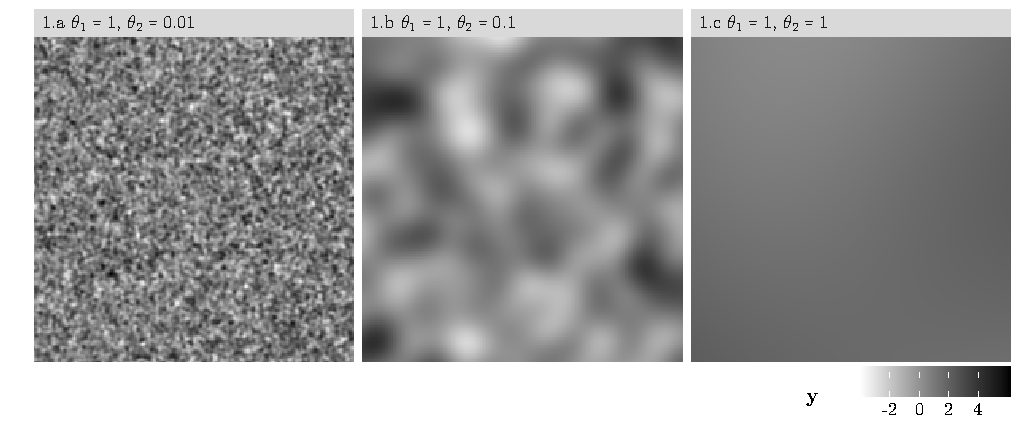
\includegraphics{fig/figure1.pdf}

    \vspace{-.4cm}
    {\footnotesize For each realisation $\signal$ of the random process $\Signal$, for each $\position$ in $\Pop$, the value of $\signal[\position]$ is color coded with a grayscale gradient.}
%\end{mdframed}
\end{figure}




\subsection{Sample, design and design variable} \label{sec:design}

\subsubsection{Fixed designs and design variables}

By definition a design $\design$ is a probability distribution on $\toPop$.
A sample $\Sample$ drawn from $\design$ is a random variable or point process of distribution $\design$, e.g. a random variable $\Sample$ such that $\mathrm{P}^\Sample=\design$. 
Define the size $\Samplesize=\mathrm{size}\circ\Sample$ of the sample $\Sample$. The sample density with respect to $\dominantUbar$, is defined by:
$(\derive P^\Sample)/(\derive\dominantUbar)(\position)=P(N=n)\times(\derive P^{\Sample\mid N=n})/(\derive\dominantU^{\otimes\{1,\ldots,n\}})(\position)$, if $\position\in\Pop^{\{1,\ldots,n\}}$, $P(N=0)$ if $\position=\mathbf{0}$. 
%For example, let $\intensity:(\Pop,\dominantU)\to(\mathbb{R}^+,\mathrm{Lebesgues}(\mathbb{R}^+))$ be a measurable function , then a Poisson point process \citep[p.~ 45]{CoxIshamPointProcesses}) with intensity $\pi$ follows a finite or discrete design if the support of $\dominantU$ is finite. The distribution of a Poisson process when the support of $\dominantU$ is finite is a design that corresponds to with replacement sampling. Confusingly, in the literature on survey sampling, Poisson sampling \citep[p.~85]{SarndalSwensonWretman1992} corresponds to a finite design where each unit $\position$ such that $\pi(\position)>0$ is drawn independently with a fixed probability $\pi(\position)$, and is thus a without replacement design.
A fixed design variable is a function $\desvar:\Pop\mapsto \DesvarSpace$.
A fixed size design $\design$ is usually defined as a function of a fixed design variable, and characterised by its density with respect to $\dominantUbar$. For example, 
the Probability Proportional to Size $\desvar$ With Replacement and size $n$ ($\mathrm{PPSWR}(\desvar,n)$) design, with $\DesvarSpace=[0,+\infty)$ is characterized by:  
\begin{equation}\label{eq:ppswr}\left(\derive P^{\Sample}/\derive\dominantUbar\right)(\position)=\left(\int_U \left(\desvar[\position']\right)\mathrm{d}\dominantU (\position')\right)^{-\samplesize}
\left(\prod_{\ell=1}^\samplesize\left(\desvar[\position(\ell)]\right)\right)\text{ if }\position\in\Pop^{\{1,\ldots,n\}},~0\text{ otherwise.}
\end{equation}
The point process $\Sample$ characterized by Equation \eqref{eq:ppswr} is a binomial point process of $\samplesize$ points in $\Pop$ with intensity $\Pop\to\mathbb{R}, \position\to\left(\left(\desvar.\dominantU\right)\left(\Pop\right)\right)^{-1}\desvar[\position]$, which we abbreviate by $\Sample\sim\mathrm{bpp}\left(\desvar,10\right)$. Simple random sampling with replacement is a binomial point process with a constant intensity.  For simplicity, we only consider exchangeable sample designs, in the sense that $\forall \samplesize\in\mathbb{N}$, for all permutation $\permutation$ of $\{1,\ldots,n\}$. $P^{S\mid\Samplesize=\samplesize}=P^{S[\permutation]\mid \Samplesize=\samplesize}$. %Pdesigns such that: 
%This general definition includes design for with and without replacement sampling and fixed and random size sampling. 
For example, given a measurable real function $\desvar :\Pop \to\mathbb{R}$, a spatial Poisson Process of intensity $\desvar$ is a point process 
$S:\Omega\to\bigcup_{\samplesize\in\mathbb{N}}\Pop^{\samplesize}$, such that 
for all $\dominantU$-measurable subset $\subsetA$ of $\Pop$, \begin{equation}\label{eq:poissonprocess}
S\sim\mathrm{Ppp}(\desvar)\Leftrightarrow
\mathrm{cardinality}(\Sample^{-1}[\subsetA])\sim \mathrm{Poisson}\left((\desvar.\dominantU)\left(\subsetA \right)\right),
\end{equation}

where $\Sample^{-1}[\subsetA]$  is the random variable with domain the finite subsets of $\Pop$ defined by: $\omega\mapsto\{\ell\in\{1,\ldots,\Samplesize(\omega)\};(\Sample(\omega))(\ell)\in \subsetA\}$ if $\Samplesize(\omega)>0$, $\emptyset$ otherwise.

The density of such process with respected to $\bar\dominantU$ is defined, for $\samplesize\in\mathbb{N}$, $\position\in \toPop$, by:
\begin{equation}
\density_{\Sample}(\position)=\left(\size (\position)!\right)^{-1}\exp\left(-\left(\desvar.\dominantU\right)(\Pop)\right)
\prod_{\ell\in\mathrm{domain}(\position)}
\desvar[\position(\ell)].
\end{equation}



%
%The Poisson Point process is such that for two measurable subsets $\subsetA_1$ and $\subsetA_1$  of $\Pop$, 
%$\subsetA_1\cap\subsetA_2=\emptyset\Rightarrow \left(\mathrm{\cardinality}(\subsetA_1\cap\Sample)\perp\mathrm{\cardinality}(\subsetA_2\cap\Sample))$, which is not necessarily the case for each Point Process (for example fixed strictly positive size point processes

%When there exists $\position(1),\ldots,\position_N\in\Pop$ such that $\dominantU=\mathrm{Dirac}_{\{\position(1),\ldots,\position_N}\}$, simple random sampling is  is finite and 

%
%Tables {\ref{tab:oiurhgoieruhgierug}} and 
%\ref{tab:oijgoirejoier} provide examples of continuous and finite population designs. 
%%Notice that the same name is used in the literature for finite or continuous population designs, without contradiction. We put them there as one goal is to establish a parallel between existing theoretical work between finite population and continuous population sampling.
%
%\begin{table}[H]\label{tab:oiurhgoieruhgierug}
%\caption{Continuous population fixed size designs}
%
%\small
%\setlength{\tabcolsep}{8pt}
%\renewcommand{\arraystretch}{1.8}
%
%\newcolumntype{b}{X}
%\newcolumntype{s}{>{\hsize=.1\hsize}X}
%
%\begin{tabularx}{\textwidth}[t]{ssb}
%\hline
%\multicolumn{3}{p{\dimexpr\linewidth-\tabcolsep-\arrayrulewidth}}{Name}\\                 &$\DesvarSpace$ & $\mathrm{d} P^{\Sample[\{1,\ldots,n\}]}/\mathrm{d}\dominantU^{\otimes n}(\position)$\\
%\hline
%\hline
%\multicolumn{3}{p{\dimexpr\linewidth-\tabcolsep-\arrayrulewidth}}{Probability Proportional to Size $\desvar$ With Replacement (PPSWR)}\\                 & $[0,+\infty)$ & $\left(\int_U \left(\desvar[\position']\right)\mathrm{d}\dominantU (\position')\right)^{-n}
%\left(\prod_{\ell=1}^n\left(\desvar[\position(\ell)]\right)\right)$\\
%\hline 
%\multicolumn{3}{p{\dimexpr\linewidth-\tabcolsep-\arrayrulewidth}}{Sytematic sampling, $\samplesize=(n')^2$ }\\&$\{1\}$                 &
%$\left\{\begin{array}{ll}(n!)^{-1} n &\text{ if }\position\in\left\{(\position_0+(n')^{-1}\alpha)_{\alpha\in \{0,\ldots,n'-1\}^2}\mid\position_0\in [0,1/n']^2\right\}\\0& \text{ otherwise.}\end{array}\right.$\\
%\hline 
%\multicolumn{3}{p{\dimexpr\linewidth-\tabcolsep-\arrayrulewidth}}{Simple Random Sampling}\\                 & ${1}$ & $\dominantU^{}\left(\int_\Delta \left(\desvar[\position']\right)\mathrm{d} (\position')\right)^{-n}
%\mathds{1}_\Delta(\position)$\\
%\hline 
%\end{tabularx}
%
%\end{table}
%
%
%\begin{table}[H] \label{tab:oijgoirejoier}
%\caption{Finite population fixed size  designs}
%
%
%\setlength{\tabcolsep}{8pt}
%\renewcommand{\arraystretch}{1.8}
%
%\begin{tabular}{lll}
%\hline
%Name                 &$\DesvarSpace$ & $\mathrm{d} P^{\Sample[\{1,\ldots,n\}]}/\mathrm{d}\dominantU^{\otimes n}(\position)$\\
%\hline
%\hline
%PPSWR &$\mathbb{R}^+$ & $\left(\int_U \Desvar[\position']\mathrm{d}\dominantU (\position')\right)^{-n}
%\left(\prod_{\ell=1}^n\Desvar[\position(\ell)]\right)$\\
%\end{tabular}
%\end{table}


\subsubsection{Random design variables, sample and random design}
In practice, the design parameter $\desvar$ is modeled as the output of a random process $\Desvar:\Omega\to(\Pop\to \DesvarSpace)$ that we will refer to as the design variable.
The selection process, when controlled, is in practice a function of an auxiliary variable, called design variable, that is a process defined on the same space $\Pop$. When the selection process is not chosen by the experimenter it can also be modelled as a function of such a process, that can be observed, partially observed or latent. In practice, it may not be reasonable to assume independence of the the design and study variables $\Desvar$ and $\Signal$.


The design is by definition a random variable with domain the set of probability distributions on  $\toPop$. The sample is a random variable $\Sample$ with domain $\toPop$ such that the distribution of $\Sample$ conditionnaly to the design \emph{is} the design, e.g:
$$P^\Design-a.s.(\design),~P^{\Sample\mid \Design=\design}=\design.$$

%In the following, we assume that $P^\Desvar$ is such that $P^\Sample$ is the  uniform distribution on $\Pop^n$: unconditionally on $Z$, the selection is uniform <<< this is wrong.
For a point process $\Sample$ with values in the measured space $(\Pop,\dominantU)$, for a random variable $W$, define $\Intensity_{S\mid W=w}$ as the intensity measure of $\Sample$ conditionally to $W=w$ with respect to the measure on $\Pop$, where for each measurable subset $\subsetA$ of $\Pop$, $\Intensity_S(A)=\mathrm{E[\mathrm{cardinality}(S^{-1}[A])\mid W=w]}$, and $\intensity_S$ as the density of $\Intensity_S$ with respect to $\dominantU$: $\intensity_S=\derive\Intensity_S/\derive\dominantU$.
%We also assume that the design follows the following exchangeability condition: for all $\samplesize\in\mathbb{N}$, for any permutation $\sigma$ of $\{1,\ldots,n\}$, for all measurable subset A of $(\{1,\ldots,n\}\to \Pop)$, for all $\omega\in\Omega$,
%$D(\omega)(A)=D(\omega)(\sigma.A)$, where $\sigma.A(k)=A(\sigma(k))$. 

%\subsubsection{Sample indicator}
%
%The sample indicator is the random variable $I$ defined by: for a subset $A$ of $\Pop$, $I[A]=1$ if $A\subset \Sample$, $0$ otherwise.




\subsubsection*{Example with simulations (continued): distribution of $\Desvar$ conditionally on $\Signal$}
We assume that 
$\Desvar$ satisfies:
$$\Desvar=\mathrm{exp}\left(\alpha+\beta\Signal+\gamma \varepsilon\right),$$
where $\alpha$,  $\beta$, $\gamma$ are real positive numbers, 
$\varepsilon:\Omega\to\left(\Pop\to\mathbb{R}\right)$
is a Gaussian process with mean:
$\mu=0$ and Gaussian covariogram of parameters $c_0=0,c_1=5, c_2=10$. 

The variable $\signal:\Pop\to\mathbb{R}$ (resp $e:\Pop\to\mathbb{R}$) is generated once by sampling from $\Signal$ (resp $\varepsilon$). The variable $\desvar=\exp\left(\alpha+\beta\signal+\gamma\mathbf{e}\right)$ is computed for 3 different values of the vector 
$(\alpha,\beta, \gamma)$: $\left(\log(10),0,0\right)$, $\left(\log(10)-(0.5^2+0.3^2),0,\sqrt{0.5^2+0.3^2}\right)$, and $\left(\log(10)-(0.5^2+0.3^2),0.5,0.3\right)$. Two samples are drawn, one following $\design=\mathrm{bpp}(\desvar,10)$ and the other following $\design=\mathrm{Ppp}(\desvar)$. 
The variables $\desvar$ and $\signal$ and the two samples are mapped in figures \ref{fig:oaijsfdwefweoij} and \ref{fig:jointmarginaldensitiesYZ}. Sampled units tend to concentrate where the sampling intensity is the highest.


\begin{figure}[H]
%\begin{mdframed}
    \caption{Heat maps of the design variable $\desvar$ and plot of realisations of $\Sample$ for three different design variables and designs.}
    \label{fig:oaijsfdwefweoij}
    \hspace{-.6cm}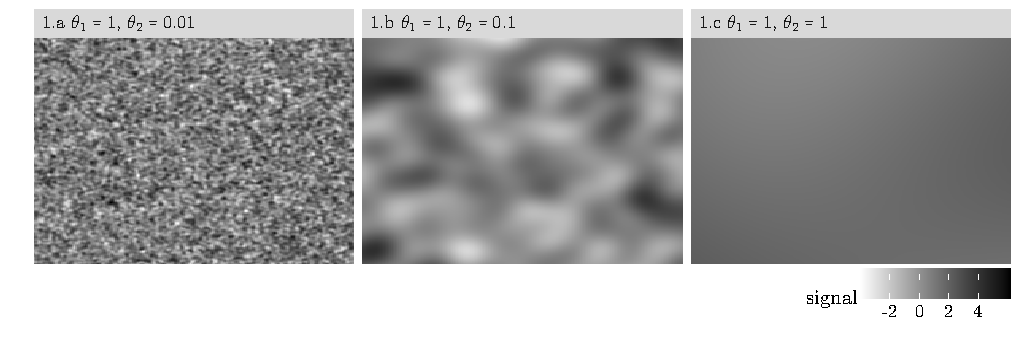
\includegraphics{fig/figure2.pdf}
    \vspace{-1cm}
    
    
    \footnotesize{
    
%
Sub-figures correspond to the  heatmap of a design variable $\desvar$ (Sub-figures 2.a, 2.b, 2.c) to the heatmap of $\signal$ (Sub-figure 2.d) and the plot of the samples (circle and triangle dots) drawn according to the two different designs. The values of $(\alpha, \beta ,\gamma)$ for each sub-figure are: 2.a: $(\log(10),0,0)$, 2.b:$(\log(10)-(0.5^2+0.3^2),0,\sqrt{0.5^2+0.3^2})$, 2.c: $(\log(10)-(0.5^2+0.3^2),0.5,0.3)$.}
%\end{mdframed}

\end{figure}

\begin{figure}[H]
%\begin{mdframed}
\caption{Joint and marginal densities of $\desvar$ and $\signal$}\label{fig:jointmarginaldensitiesYZ}
\includegraphics{fig/figure3.pdf}
\footnotesize{
 Each sub-figure contains the scatter plot of  $\left\{\left(\desvar[\position],\signal[\position]\right):\position\in\mathrm{Grid}\right\}$, where $\mathrm{Grid}$ is a regularly spaced grid of $\Pop$. The values of $(\alpha, \beta ,\gamma)$ for each Sub-figure are: 3.1: $(\log(10),0,0)$, 3.2:$(\log(10)-(0.5^2+0.3^2),0,\sqrt{0.5^2+0.3^2})$, 3.3: $(\log(10)-(0.5^2+0.3^2),0.5,0.3)$. The vertical axis corresponds to $\signal$, the vertical to $\desvar$. The marginal plots correspond to the density of $\desvar$ (right margin) and to the densities of $\signal$ (bottom margins).}
%\end{mdframed}
\end{figure}




\subsection{Observations}
The observation consists of the realisations of the random variables $\Sample$ and $\Signal[\Sample]$. 
%$(\Sample[\ell],\Signal[\Sample[\ell]])_{\ell\in\{1,\ldots,\Sampleindex}$
%Observations $(\Sample,\Signal[\Sample])=(\Sample[\ell],\Signal[\Sample[\ell]])_{\ell=1,\ldots,n}$ can be seen as a point process in $\Pop\times\SignalSpace$ and its intensity is defined as the Radon Nikodym derivative of $\Intensity_S$ with respect to the measure $\dominantU\otimes\dominantY$.


\section{``Sample" vs ``Population''  distribution of the signal}\label{sec:sampledistribution}

The observation consists of the realisations of the random variables $\Sample$ and $\Signal[\Sample]$. In this section, we derive the distribution of the observed values of the signal on the sample, (e.g. the distribution of $\Signal[\Sample]$) from  the distribution of the design variable conditionally $\Desvar$ to the signal $\Signal$ and the function that links the design to the design variable, or equivalently the distribution of the sample $\Sample$ conditionally to the design variable $\Desvar$. We resort to  the Bayes formula to express the density of $(\Signal[\Sample],\Sample)$ in $(\signal,\position)$,   as the product of the density of the sample $\Sample$ in $\position$ conditionally on $\Signal[\position]=\signal$ by the density of the signal $\Signal[\position]$ in $\signal$. 
\subsection{Density ratio}
\subsubsection{Definition and properties}
%In this section, we derive the distribution of the observed values of the signal on the sample, (e.g. the distribution of $\Signal[\Sample]$) from  the distribution of the design variable conditionally $\Desvar$ to the signal $\Signal$ and the function that links the design to the design variable, or equivalently the distribution of the sample $\Sample$ conditionally to the design variable $\Desvar$. To this end, we proceed step by step and resort to the Bayes formula. 
We start with the following definition.


%{\color{red} Do we need the notation g ? the idea is that $g$ is the density for the sample. I am in favour of creating a command and call it $\pi$ instead.} 


\begin{definition}
For a random set $\Sampleindex$, 
define
$\densityratio_{\Sampleindex}(.\mid.)$ as any function that satisfies:

\begin{equation}
P^{(\Sample_\Sampleindex,\Signal[\Sample_\Sampleindex])}-\text{a.s}(\position,\signal),~\density_{\Signal[\position]\mid\Sample_\Sampleindex=\position}\left(\signal\right)=
    \density_{\Signal[\position]}\left(\signal\right)
    \densityratio_{\Sampleindex}\left(\position\mid  \signal\right)\label{eq:owijoj}
\end{equation}

\end{definition}


\begin{property}\label{prop:ieuhierhgi}
%Let $\Sampleindex$ be a non random finite subset of $\mathbb{N}$, then
\begin{equation}
P^{(\Sample_\Sampleindex,\Signal[\Sample_\Sampleindex])}-\text{a.s}(\position,\signal),~~~
\densityratio_{\Sampleindex}\left(\position \mid \signal\right)
         \density_{\Sample_\Sampleindex}\left(\position\right)=
    \density_{\Sample_\Sampleindex\mid \Signal[\position]}\left(\position|\signal\right)
\end{equation}


\end{property}

\begin{proof}
From the Bayes formula:
\begin{eqnarray}
\density_{\Signal[\position]\mid\Sample_\Sampleindex =\position }\left(\signal\right)
&=&(\density_{\Sample_\Sampleindex }(\position))^{-1}~\density_{\Signal[\position],\Sample_\Sampleindex }(\signal,\position)\\
&=&(\density_{\Sample_\Sampleindex }(\position))^{-1}~
\density_{\Sample_\Sampleindex \mid\Signal[\position]}(\position\mid \signal)~
\density_{\Signal[\position]}(\signal)\label{eq:oijoijsf}
\end{eqnarray}


So, combining Equations \eqref{eq:oijoijsf} and  \eqref{eq:owijoj}:
\begin{equation}
{\densityratio_{\Sampleindex}\left(\position \mid \signal\right)}
=(\density_{\Sample_\Sampleindex }(\position))^{-1}
~\density_{\Sample_\Sampleindex \mid\Signal[\position]}(\position\mid \signal).
\end{equation}
\end{proof}%

Property \ref{prop:ieuhierhgi} provides an interpretation of $\densityratio_\Sampleindex(\signal\mid \position)$ as the probability that the draws indexed by $\Sampleindex$ correspond to the sample $\position$ conditionally on the values of $\Signal$ in $\position$ divided by the same probability unconditionally on the values of $\Signal$. 
In this sense, the density ratio $\densityratio_\Sampleindex(\signal\mid \position)$ is a relative probability of selection.
%$\densityratio_{\Sampleindex}(\position\mid\signal)$




%Besides,
%\begin{equation}\label{eq:iurhiehgieurhg}
%\density_{\Sample_\Sampleindex }(\position)=
%\int \density_{\Sample_\Sampleindex \mid \Signal[\position]}(\position\mid \signal)~ \density_{\Signal[\position]}(\signal)~
%\derive \dominantY^{\otimes \Sampleindex}(\signal)
%\end{equation}
\begin{property}
The density ratio $\densityratio$ can be derived from the distribution of $\Desvar$ via:

\begin{eqnarray}\label{eq:rho_expression}
\densityratio_{\Sampleindex}(\position\mid\signal)&=&\left({\int
         \density_{\Sample_\Sampleindex\mid \Desvar}\left(\position|\desvar\right)\derive P^{\Desvar}}\right)^{-1}{\int\density_{\Sample_\Sampleindex\mid \Desvar}(\position\mid\desvar)\derive P^{\Desvar\mid\Signal[\position]=\signal}(\desvar)}
\label{eq:oigjeogjio}\end{eqnarray}
\end{property}

\begin{property}\label{prop:indeprho}
If $\Desvar$ and $\Signal$ are independent, then $\densityratio_K(\position\mid\signal)=1$.
\end{property}
\begin{proof}
$\Desvar\perp\Signal\Rightarrow P^\Desvar=P^{\Desvar\mid\Signal[\position]=\signal}$. Replacing $P^{\Desvar\mid\Signal[\position]=\signal}$ by $P^{\Desvar}$ in the numerator of Equation \eqref{eq:rho_expression} yields  $\densityratio_K(\position\mid\signal)=1$.
\end{proof}

\subsubsection{Computation of $\densityratio$ on a Case study}
In this subsection, we use the framework of Example \ref{example:2.4} to illustrate the properties and provide graphical representations of the density ratio.
We remind that in this framework, $\Sample\sim \mathrm{Ppp}(\Desvar)$ or  $\Sample\sim \mathrm{bpp}(\Desvar,\samplesize)$.
Conditionally on $\Signal[\position]=\signal$, $\Desvar$ is a log normal random process with distribution characterized by 
$E[\log(\Desvar[\position'])\mid \Signal[\position]=\signal]=\paramnuisance_0+\paramnuisance_1(\mu+\Sigma_{\position',\position}\Sigma_{\position,\position}^{-1} (\signal-\mu))$ and 
$\mathrm{Var}[\log(\Desvar[\position'])\mid \Signal[\position]=\signal]=\paramnuisance_2^2\provar_{\varepsilon;\position',\position'}+\paramnuisance_1^2\left(\provar_{\Signal;\position',\position'}-\provar_{\Signal;\position',\position}\provar_{\Signal;\position,\position}^{-1}\provar_{\Signal;\position,\position'})\right)$.
\begin{proof}
See Appendix \ref{sec:A.owifjoeij}
\end{proof}

For $\position=\mathbf{0}$  and  $\signal=\mathbf{0}$,
\begin{eqnarray*}
\lefteqn{\density_{\Sample_{\{1\}}\mid\Signal[\mathbf{0}]=\mathbf{0}}(\mathbf{0}))}\\&=&
\density_{\Sample_{\{1\}}}(\mathbf{0})\\
&=&\left|\begin{array}{ll}
\int \exp\left(-(\desvar.\dominantU)(\Pop)\right)\derive P^{\Desvar}(\desvar)&\text{if }\Sample\sim\mathrm{Ppp}(\Desvar)\\
0&\text{if }\Sample\sim\mathrm{bpp}(\Desvar,\samplesize),\end{array}\right.
\end{eqnarray*}
so $\densityratio_{\{1\}}(\mathbf{0}\mid\mathbf{0})=
\density_{\Sample_{\{1\}}\mid\Signal[\mathbf{0}]=\mathbf{0}}(\mathbf{0})/\density_{\Sample_{\{1\}}}(\mathbf{0})=
1$.
More generally, for any random set $\Sampleindex$, $\densityratio_{\Sampleindex}(\mathbf{0}\mid\mathbf{0})=1.$
When $\Sample\sim \mathrm{Ppp}(\Desvar)$,
for $\position\in\Pop^{\{1\}}$, as a consequence of Equations \eqref{eq:iduhifduewer} and \eqref{eq:sgiushdiuh},
\begin{eqnarray*}
\lefteqn{\densityratio_{\{1\}}(\position\mid\signal)}\\&=&\frac{
\int 
\left(\sum_{\samplesize\geq 1} (\samplesize!)^{-1}(\desvar.\dominantU)(\Pop)^\samplesize\right)\times \exp\left(-(\desvar.\dominantU)(\Pop)\right)
\left((\desvar.\dominantU)(\Pop)\right)^{-1}\desvar(\position(1))\derive P^{\Desvar\mid \Signal[\position]}(\desvar\mid\signal) 
}{
\int 
\left(\sum_{\samplesize\geq 1} (\samplesize!)^{-1}(\desvar.\dominantU)(\Pop)^\samplesize\right)\times \exp\left(-(\desvar.\dominantU)(\Pop)\right)
\left((\desvar.\dominantU)(\Pop)\right)^{-1}\desvar(\position(1))\derive P^{\Desvar}(\desvar) 
}\\&=&\frac{
\int 
\left(1-\exp\left(-(\desvar.\dominantU)(\Pop)\right)\right)
\left((\desvar.\dominantU)(\Pop)\right)^{-1}\desvar(\position(1))\derive P^{\Desvar\mid \Signal[\position]}(\desvar\mid\signal) 
}{
\int 
\left(1-\exp\left(-(\desvar.\dominantU)(\Pop)\right)\right)
\left((\desvar.\dominantU)(\Pop)\right)^{-1}\desvar(\position(1))\derive P^{\Desvar}(\desvar)\phantom{11111} 
}\\&=&\frac{
\int 
\left(1-\exp^{-\int \exp\left( \paramnuisance_0+\paramnuisance_1\Signal[\position']+\paramnuisance_2\varepsilon[\position']\right)\derive\dominantU(\position')}\right)
\left(\int \exp^{-\paramnuisance_1(\Signal[\position']-\signal)-\paramnuisance_2(\varepsilon[\position']-\varepsilon[\position])}\derive\nu(\position')\right)^{-1}\derive P^{\Signal,\varepsilon\mid \Signal[\position]=\signal} 
}{
\int
\left(1-\exp^{-\int \exp\left( \paramnuisance_0+\paramnuisance_1\Signal[\position']+\paramnuisance_2\varepsilon[\position']\right)\derive\dominantU(\position')}\right)
\left(\int \exp^{-\paramnuisance_1(\Signal[\position']-\Signal[\position(1)])-\paramnuisance_2(\varepsilon[\position']-\varepsilon[\position(1)])}\derive\nu(\position')\right)^{-1}\derive P^{\Signal,\varepsilon}\phantom{11111} 
}
\end{eqnarray*}

and for  $\position\in\Pop^{\{1,2\}}$, 
\begin{eqnarray*}
\lefteqn{\densityratio_{\{1,2\}}(\position\mid\signal)}\\&=&\frac{
\int 
\frac{\left(1-(1+(\int\exp\left( \paramnuisance_0+\paramnuisance_1\Signal[\position']+\paramnuisance_2\varepsilon[\position']\right)\derive\dominantU(\position')))\right)}{\exp\left(\int\exp\left( \paramnuisance_0+\paramnuisance_1\Signal[\position']+\paramnuisance_2\varepsilon[\position']\right)\derive\dominantU(\position')\right)}\frac{
\exp^{-\paramnuisance_1(\sum_{\ell=1}^2\signal(\ell))-\paramnuisance_2(\sum_{\ell=1}^2\varepsilon[\position(\ell)])}}{
\left(\int \exp\left(-\paramnuisance_1(\Signal[\position'])-\paramnuisance_2(\varepsilon[\position'])\right)\derive\nu(\position')\right)^2
}\derive P^{\Signal,\varepsilon\mid \Signal[\position]=\signal} 
}{
\int 
\frac{\left(1-(1+(\int\exp\left( \paramnuisance_0+\paramnuisance_1\Signal[\position']+\paramnuisance_2\varepsilon[\position']\right)\derive\dominantU(\position')))\right)}{\exp\left(\int \exp\left(\paramnuisance_0+\paramnuisance_1\Signal[\position']+\paramnuisance_2\varepsilon[\position']\right)\derive\dominantU(\position')\right)}\frac{
\exp^{-\paramnuisance_1(\sum_{\ell=1}^2\Signal(\position[\ell]))-\paramnuisance_2(\sum_{\ell=1}^2\varepsilon[\position(\ell)])}}{
\left(\int \exp\left(-\paramnuisance_1(\Signal[\position'])-\paramnuisance_2(\varepsilon[\position'])\right)\derive\nu(\position')\right)^2
}\derive P^{\Signal,\varepsilon}\phantom{11111} 
}
\end{eqnarray*}

and for  $\position\in\Pop^{\{1,\ldots,\samplesize\}}$, as a consequence of Equations \eqref{eq:iduhifduewer} and \eqref{eq:sgiushdiuh2}
\begin{eqnarray*}
\lefteqn{\densityratio_{\{1,\ldots,\Samplesize\}}(\position\mid\signal)}\\&=&\frac{
\int 
\frac{\left(\int \exp\left(\paramnuisance_0+\paramnuisance_1\Signal[\position']+\paramnuisance_2\varepsilon[\position']\right)\derive\dominantU(\position')\right)^\samplesize}{\samplesize!~\exp\left(\int \paramnuisance_0+\paramnuisance_1\Signal[\position']+\paramnuisance_2\varepsilon[\position']\derive\dominantU(\position')\right)}\frac{
\exp^{-\paramnuisance_1(\sum_{\ell=1}^\samplesize\signal(\ell))-\paramnuisance_2(\sum_{\ell=1}^\samplesize\varepsilon[\position(\ell)])}}{
\left(\int \exp\left(-\paramnuisance_1(\Signal[\position'])-\paramnuisance_2(\varepsilon[\position'])\right)\derive\nu(\position')\right)^\samplesize
}\derive P^{\Signal,\varepsilon\mid \Signal[\position]=\signal} 
}{
\int 
\frac{\left(\int\exp\left( \paramnuisance_0+\paramnuisance_1\Signal[\position']+\paramnuisance_2\varepsilon[\position']\right)\derive\dominantU(\position')))\right)^\samplesize}{\samplesize!\exp\left(\int \exp\left(\paramnuisance_0+\paramnuisance_1\Signal[\position']+\paramnuisance_2\varepsilon[\position']\right)\derive\dominantU(\position')\right)}\frac{
\exp^{-\paramnuisance_1(\sum_{\ell=1}^2\Signal(\position[\ell]))-\paramnuisance_2(\sum_{\ell=1}^\samplesize\varepsilon[\position(\ell)])}}{
\left(\int \exp\left(-\paramnuisance_1(\Signal[\position'])-\paramnuisance_2(\varepsilon[\position'])\right)\derive\nu(\position')\right)^\samplesize
}\derive P^{\Signal,\varepsilon}\phantom{11111} 
}
\end{eqnarray*}



When $\Sample\sim \mathrm{bpp}(\Desvar,\samplesize)$, for $\position \in \Pop^{\{1\}}$:

\begin{equation*}
\densityratio_{\{1\}}(\position\mid\signal)=
\frac{
\int 
\left(\int \exp^{-\paramnuisance_1(\Signal[\position']-\signal)-\paramnuisance_2(\varepsilon[\position']-\varepsilon[\position])}\derive\nu(\position')\right)^{-1}\derive P^{\Signal,\varepsilon\mid \Signal[\position]=\signal} 
}{
\int
\left(\int \exp^{-\paramnuisance_1(\Signal[\position']-\Signal[\position(1)])-\paramnuisance_2(\varepsilon[\position']-\varepsilon[\position(1)])}\derive\nu(\position')\right)^{-1}\derive P^{\Signal,\varepsilon}\phantom{11111} 
}.
\end{equation*}

for $\position \in \Pop^{\{1,2\}}$:
\begin{equation*}
\densityratio_{\{1,2\}}(\position\mid\signal)=
\frac{
\int 
\frac{\exp\left(-\paramnuisance_1(\sum_{\ell=1}^2\signal(\ell)-\paramnuisance_2(\sum_{\ell=1}^2\varepsilon[\position(\ell)])\right)}{\left(\int \exp\left(-\paramnuisance_1\Signal[\position']-\paramnuisance_2\varepsilon[\position']\right)\derive\nu(\position')\right)^{2}}\derive P^{\Signal,\varepsilon\mid \Signal[\position]=\signal} 
}{
\int 
\frac{\exp\left(-\paramnuisance_1(\sum_{\ell=1}^2\Signal[\position(\ell)]-\paramnuisance_2(\sum_{\ell=1}^2\varepsilon[\position(\ell)])\right)}{\left(\int \exp\left(-\paramnuisance_1\Signal[\position']-\paramnuisance_2\varepsilon[\position']\right)\derive\nu(\position')\right)^{2}}\derive P^{\Signal,\varepsilon}\phantom{11111} 
}.
\end{equation*}


and 
for $\position \in \Pop^{\{1,\ldots,\samplesize'\}}$, $0\leq\samplesize'\leq\samplesize$:

\begin{equation*}
\densityratio_{\{1,\ldots,\samplesize'\}}(\position\mid\signal)=
\frac{
\int 
\frac{\exp\left(-\paramnuisance_1(\sum_{\ell=1}^2\signal(\ell)-\paramnuisance_2(\sum_{\ell=1}^{\samplesize'}\varepsilon[\position(\ell)])\right)}{\left(\int \exp\left(-\paramnuisance_1\Signal[\position']-\paramnuisance_2\varepsilon[\position']\right)\derive\nu(\position')\right)^{\samplesize'}}\derive P^{\Signal,\varepsilon\mid \Signal[\position]=\signal} 
}{
\int 
\frac{\exp\left(-\paramnuisance_1(\sum_{\ell=1}^{\samplesize'}\Signal[\position(\ell)]-\paramnuisance_2(\sum_{\ell=1}^{\samplesize'}\varepsilon[\position(\ell)])\right)}{\left(\int \exp\left(-\paramnuisance_1\Signal[\position']-\paramnuisance_2\varepsilon[\position']\right)\derive\nu(\position')\right)^{\samplesize'}}\derive P^{\Signal,\varepsilon}\phantom{11111} 
}.
\end{equation*}


The density ratio is a function of $\position$, $\signal$,  $\paramnuisance$, and $\parampop$.
\begin{properties}{Properties of $\densityratio$ common to Poisson and binomial point processes}
\begin{enumerate}
\item[i.] $\paramnuisance_1=0\Rightarrow \intensityratio(\position,\signal;\paramnuisance,\parampop)=1$.
\item[ii.] $\intensityratio_\Sampleindex(\position\mid\signal;\paramnuisance,\parampop)-1=o_{\paramnuisance_2\to\infty}(1)$,
\item[iii.] $\intensityratio_\Sampleindex(\position\mid\signal;\paramnuisance,\parampop)-1=o_{\parampop_{\text{scale}}\to\infty}(1)$,
\item[iv.] $\intensityratio_\Sampleindex(\position\mid\signal;\paramnuisance,\parampop)-1=o_{\parampop_{\text{scale}}\to\infty}(1)$,
\item[v.] $\intensityratio_\Sampleindex(\position,-\signal;(\parampop,(\paramnuisance_0,-\paramnuisance_1,\paramnuisance_2,\paramnuisance_{\text{scale}})=\intensityratio_\Sampleindex(\position\mid\signal;(\parampop,(\paramnuisance_0,\paramnuisance_1,\paramnuisance_2,\paramnuisance_{\text{scale}})$
\item[vi.] $\mathrm{sign}(\paramnuisance_1)=1\Rightarrow \lim_{\signal\to\infty}\intensityratio_{\{1\}}(\position\mid\signal;\paramnuisance,\parampop)=+\infty$,
\item[vii.] $\mathrm{sign}(\paramnuisance_1)=1\Rightarrow \lim_{\signal\to-\infty}\intensityratio_{\{1\}}(\position\mid\signal;\paramnuisance,\parampop)=0$,
\end{enumerate}
\end{properties}




\begin{properties}{Properties of $\densityratio$ when $\Sample\sim\mathrm{bpp}(\Desvar,\samplesize)$}
\begin{enumerate}
\item[i.] $ \intensityratio_{\{1\}}(\position\mid\signal;\paramnuisance,\parampop)=
\exp(\paramnuisance_1(\signal-\paramnuisance/2) + o_{\parampop_{\text{scale}}\to 0}(1)$.
\item[ii.] $\samplesize'\leq\samplesize\Rightarrow\intensityratio_{\{1,\ldots\samplesize'\}}(\position\mid\signal;\paramnuisance,\parampop)=
\exp\left(\paramnuisance_1(\sum_{\ell=1}^{\samplesize'}\signal(\ell)-\samplesize'\paramnuisance_1/2)\right) + o_{\parampop_{\text{scale}}\to 0}(1)$.
\end{enumerate}
\end{properties}

%{\color{red} 
%Based on those properties, we can use a proxy for $\rho:$ we fit the following 

%$$\tilde\densityratio_{\{1\}}(\signal\mid\position;\parampop,\paramnuisance)=
%1+(\exp\left(\alpha\parampop_1\signal\right)-1)
%\exp(\beta\paramnuisance_2)
%$$

%where the parameters $\alpha$ and $\beta$ depend on the scale parameter $\parampop_?$.}


The density ratio $\densityratio(\position\mid\signal)$ is the product of  two integrals as shown in Equation \eqref{eq:oigjeogjio}. No close form could be obtained for any of these two integrals. However, we can use Monte Carlo approximations to compute $\densityratio(\position\mid\signal)$.
In the case where $\Pop$ is finite, we can simulate realisations of $P^\Signal$ and  $P^\varepsilon$ on the population independently $\nrep$ times.
Let denote by $\Signal^{(\repindex)}$  and $\varepsilon^{(\repindex)}$ the $j$-th realisation of each distribution $\Signal$ and $\varepsilon$, respectively.

For $\repindex \in 1,\ldots,\nrep$, let define $\Signal_c^{(\repindex)}$ by 
$\Signal_c^{(\repindex)}[\position']=\Signal^{(\repindex)}[\position']+\provar_{\Signal;\position',\position}\provar_{\Signal;\position,\position}^{-1}(\signal-\Signal^{(\repindex)}[\position])$, which ensures that 
$P^{\Signal_c^{(\repindex)}}=P^{\Signal\mid\Signal[\position]=\signal}$ by the Matheron rule \citep{wilson2020pathwise, doucet2010note}.

Define, for a non random set $\Sampleindex$,  $\emptyset\neq\Sampleindex\subset\{1,\ldots,\samplesize\}$, 
and $\position\in\Pop^\Sampleindex$, $\signal\in\SignalSpace^\Sampleindex$, $\uple=\size(\Sampleindex)$:
$$\tilde\densityratio_{\Sampleindex}(\position\mid\signal)=
\frac{\sum_{\repindex=1}^\nrep 
    \left(\left(
    \left(\exp\left(\paramnuisance_1\Signal_c^{(\repindex)}+\paramnuisance_2\varepsilon^{(\repindex)}\right).\dominantU\right)(\Pop)\right)^{-\uple}\prod_{\ell\in\Sampleindex}\exp\left(\paramnuisance_1\signal(\ell)+\paramnuisance_2\varepsilon[\position(\ell)]\right)
    \right)}{\sum_{\repindex=1}^\nrep 
    \left(\left(
    \left(\exp\left(\paramnuisance_1\Signal^{(\repindex)}+\paramnuisance_2\varepsilon^{(\repindex)}\right).\dominantU\right)(\Pop)\right)^{-\uple}\prod_{\ell\in\Sampleindex}\exp\left(\paramnuisance_1\Signal_{\phantom{c}}^{(\repindex)}[\position(\ell)]+\paramnuisance_2\varepsilon[\position(\ell)]\right)
    \right)}.$$

In the case of a binomial point process ($\Sample\sim\mathrm{bpp}(\Desvar,\samplesize)$), the ratio of the expected values of the numerator and denominators of $\tilde\densityratio(\position\mid\signal)$ is exactly $\densityratio_\Sampleindex(\position\mid\signal)$.
The empirical variance of the summands of the numerator and numerator can be used to estimate the variance of $\tilde\densityratio(\position\mid \signal)$.


Following the aforementioned discussion, we employ a Monte Carlo simulation in order to approximate $\densityratio$ by means of $\tilde\densityratio_{\Sampleindex}(\position\mid\signal)$. As first step, we generate $J=10,000$ replications for the computation of $\tilde\densityratio_{\lbrace 1\rbrace}(\position\mid\signal)$. In Figure \ref{fig:rho_1_beta} we investigate the role of $\paramnuisance_{1}$. Toward this end, $\paramnuisance_{2}$ is kept fixed to 1, and $\paramnuisance_{1}$ varies while $\signal$ is kept fixed as well. This procedure is done for different levels of $\signal$. As expected, the value of $\tilde\densityratio_{\lbrace 1\rbrace}(\position\mid\signal)$ at $\paramnuisance_{1}=0$ is always equal to 1. Indeed, we recall that $\paramnuisance=0$ implies independence between $\Signal$ and $\Desvar$. When $\paramnuisance_{1}$ differs from zero, $\tilde\densityratio_{\lbrace 1\rbrace}(\position\mid\signal)$ is different from 1, hence reflecting the fact that dependence between $\Signal$ and $\Desvar$ introduces bias. In particular, we can observe that as $\paramnuisance_{1}$ approaches infinity, $\tilde\densityratio_{\lbrace1\rbrace}(\position\mid\signal)$ approaches zero. Also, for positive values of $\signal$, the maximum is achieved around $\paramnuisance_{1}=\signal$. The same analysis is performed for the behavior of $\paramnuisance_{2}$, where $\paramnuisance_{1}$ is kept fixed to 1, and different values of $\signal$ are fixed while $\paramnuisance_{2}$ varies. We report the results in Figure \ref{fig:rho_1_gamma}. When $\paramnuisance_{2}=0$, $\tilde\densityratio_{\lbrace 1\rbrace}(\position\mid\signal)$ is different from zero. This reflects the fact that $\paramnuisance_{1}$ is fixed to 1. As $\paramnuisance_{2}$ increases, the effect of $\paramnuisance_{1}$ decreases and $\tilde\densityratio_{\lbrace 1\rbrace}(\position\mid\signal)$ tends to 1. We then turn the attention to $\tilde\densityratio_{\lbrace 1,2\rbrace}(\position\mid\signal)$. $J=4,000$  replications are generated and values of $\tilde\densityratio_{\lbrace 1,2\rbrace}(\position\mid\signal)$ are computed for four different couples of units, which have an Euclidean distance (between the two points) of 0.018, 0.074, 0.357, and 0.711, respectively. In Figure \ref{fig:rho_12} the contours of the surface generated by the values of $\tilde\densityratio_{\lbrace 1,2\rbrace}(\position\mid\signal)$ when the two values of $\signal$ vary are plotted.


\begin{figure}[H]
\centering
\caption{Representation of $\tilde\densityratio_{\lbrace 1\rbrace}(\position\mid\signal)$ when $\Sample \sim \mathrm{bpp}(\Desvar,\samplesize)$, $\paramnuisance_{2} = 1$, and $\paramnuisance_{1}$ varies. The value of $\signal$ is reported on top of the corresponding graph.}
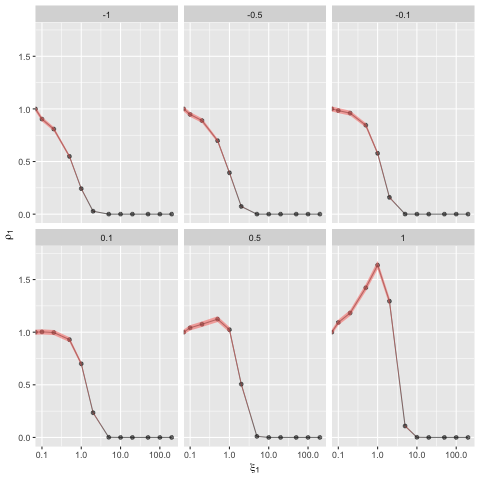
\includegraphics[width = 0.7\textwidth]{fig/rho_1_beta.png}
\label{fig:rho_1_beta}
\end{figure}

\begin{figure}[H]
\centering
\caption{Representation of $\tilde\densityratio_{\lbrace 1\rbrace}(\position\mid\signal)$ when $\Sample \sim \mathrm{bpp}(\Desvar,\samplesize)$, $\paramnuisance_{1} = 1$, and $\paramnuisance_{2}$ varies. The value of $\signal$ is reported on top of the corresponding graph.}
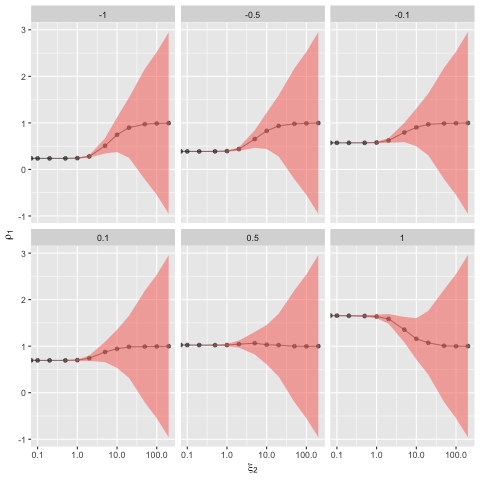
\includegraphics[width = 0.7\textwidth]{fig/rho_1_gamma.png}
\label{fig:rho_1_gamma}
\end{figure}

%\begin{example}{(continued)}
%We remark that $\paramnuisance_1=0$ implies the independence of $\Desvar$ and $\Signal$. 
%By continuity
%\begin{figure}[H]
%\caption{Estimation of $\densityratio_{\{1\}}(\signal\mid\position;\parampop,\paramnuisance)$}
%\end{figure}
%\end{example}

\begin{figure}[H]
\centering
\caption{Representation of $\tilde\densityratio_{\lbrace 1,2\rbrace}(\position\mid\signal)$ when $\Sample \sim \mathrm{bpp}(\Desvar,\samplesize)$, $\paramnuisance_{1} = 1$, $\paramnuisance_{2}=1$, and for four different couples of points.}
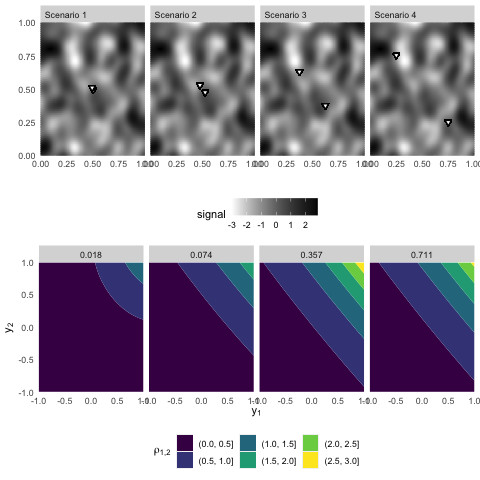
\includegraphics[width = 0.8\textwidth]{fig/rho_12_contour.png}
\label{fig:rho_12}
\end{figure}







%\subsection{Distribution of $\Signal[\Sample]$}
\subsection{Density ratio $\densityratio$ and distribution of \texorpdfstring{$\Signal[\Sample]$}{Y[\Sample_\Sampleindex]} }
The density of $\Signal[\Sample_\Sampleindex]$ with respect to $\dominantYbar$ is defined by
\begin{eqnarray}\density_{\Sample_\Sampleindex,\Signal[\Sample_\Sampleindex]}(\position\mid\signal)&=& \density_{\Signal[\position]}(\signal)~\times~\densityratio_{\Sampleindex}(\position\mid\signal)~\times~\density_{\Sample_\Sampleindex}(\position).\label{eq:iuhsdewripeowi}\\
&=& \density_{\Signal[\position]}(\signal)~\times~\density_{\Sample_\Sampleindex\mid\Signal[\position]}(\position\mid\signal).\label{eq:iuhsdewripeowi2}
\end{eqnarray}

In particular,
\begin{eqnarray}\density_{\Sample,\Signal[\Sample]}(\position\mid\signal)&=& \density_{\Signal[\position]}(\signal)~\times~\densityratio_{\{1,\ldots,\Samplesize\}}(\position\mid\signal)~\times~\density_{\Sample}(\position)
.\label{eq:iuhsdewripeowi3}
\end{eqnarray}


So when $\Desvar\perp\Signal$,
\begin{equation}\density_{\Signal[\Sample_\Sampleindex]\mid\Sample_\Sampleindex}(\signal\mid \position)= \density_{\Signal[\position]}(\signal).\label{eq:iuhsdewripeowi2}\end{equation}

\cite{pfefferman_1992} explore  the case where
$K=\{1\}$ and the spatial process satisfies the  population independence assumption:

$\forall \position\in\Pop^{\{1,\ldots,\samplesize\}}$, such that $(\position[1],\ldots,\position[\samplesize])$ are two by two  distinct,

\begin{equation}
(\Signal[\position[1]],\ldots,\Signal[\position[\samplesize]])\text{ are i.i.d variables}.
\label{eq:independenceassumption}
\end{equation}

To the ``population'' distribution, which is the distribution of $\Signal$ that satisfies Equation \eqref{eq:independenceassumption} with probability density function $\density_{\Signal[\position]}$ for $\position \in\Pop^{\{1\}}$, \cite{pfefferman_1992} oppose the sample distribution, that is the  distribution of a random variable $\Signal^\star$ that satisfies Equation \eqref{eq:independenceassumption}  and with probability density function  $\densityratio_{\{1\}}\density_{\Signal[\position]}$ for $\position \in\Pop^{\{1\}}$.

The random variable $\Signal^\star$ ''does not exist``, in the sense that if the observer could measure $\Signal[\position]$ for all values of $\position$ on $\Pop$, of for values of $\position$ in a non informative sample (e.g. such that $\densityratio=1$), the distribution of  observations would have probability density $\density_\Signal[\Sample]$.
With an informative sample, the observations are similar to what one would observe with a simple random sample and if the population was following $P^{\Signal^\star}$ and not $P^\Signal$. The distribution of $\Signal^\star$ is called by \cite{pfefferman_1992} the ``sample'' distribution.

In the case of a spatial process, can we define a sample distribution ?

Sometimes not, due to the property pointed out in Remark \ref{remark:K1subsetK2}:
the finite dimensional probability density functions 
$\densityratio{\{1,\ldots,\samplesize\}}(\position\mid\signal)\density_{\Signal[\position](\signal)}$ are not necessarily the finite dimensional densities of the same random process distribution.
A sufficient condition for the finite dimensional densities to be finite dimensional probability functions of the same process is that the sample size is fixed.
But then, there is not necessarily unicity of the random process distribution that have these finite dimensional probability density functions, as they are only defined up to the dimension equal to the sample size.



Generalising \cite{pfefferman_1992}, the selection is non informative when $\forall \uple\in\mathbb{N}$ $P^{\Signal[\Sample],\Sample}-\text{a.s.}(\signal,\position)$, $$\densityratio_{\{1,\ldots,\Samplesize\}}(\position\mid\signal)=1.$$ In this case, we consider that the sample distribution corresponds to the population distribution.


In the general case, we then define the sample distribution as a
collection of finite dimensional distributions with respective p.d.f.'s
$\densityratio{\{1,\ldots,\samplesize'\}}(\position\mid\signal)\density_{\Signal[\position](\signal)}$, with\\ $\samplesize'\in\left\{\{1,\ldots,\max\left(\Samplesize(\Samplesize^{-1}(\mathbb{N}))\right)\right\}$. 



%\subsection{Sample Variogram}
\subsection{Sample counterpart of distribution characteristics}

Even if the definition of the sample distribution is not the distribution of a random process on $\Pop$, we propose to define the sample counterpart of different characteristics of the population distribution as for example %the intensity and 
the sample semivariogram.


In a non spatial framework,  \cite{pfefferman_1992} differentiates the characteristics of the distribution of one variable when observed on the sample, and the characteristics of the same variable when observed on the population. The terminology to differentiate consists in adding ``populatio'' or ``sample'' to the name of the characteristic. For example, the population probability density function (pdf) is the equivalent  $\density_{\Signal[\position]}$ in our example, and the sample pdf is the density $\density_{\Signal[\Sample[1]]}$. \cite{bonnery2012uniform} and \cite{dbb1} investigate further this concept of population and sample characteristics.
In the following, we provide the definition of the sample characteristics of the distribution of $\Signal$ that are meaningful in the context of a spatial model.



%\subsubsection{Sample probability density function, and cumulative density function}
Some characteristics of the distribution of $\Signal$ can be  defined as expected values of a transformation of the values of $\Signal$ on all samples of $\Pop$.
For example, we have seen that the distribution of 
a Gaussian process is characterised by $E[\Signal[\position]]$ for $\position\in \Pop$ and
$\Var[\Signal[\position]]$ for $\position\in \Pop^{\{1,2\}}$. Those characteristics can be obtained by integrals of the form $\int g(\signal[\position]) \density_{\Signal[\position]}(\signal[\position])\derive\dominantYbar$, which themselves can be seen as expected values of statistics derived from the values of $\Signal$ on a simple random sample with replacement.
Those characteristics are called ``population characteristics''. Their sample counterparts are obtained by substituting $ \density_{\Signal[\position]}$ by $\densityratio_{\{1,\ldots,\size(\position)\}}\density_{\Signal[\position]}$, and can be interpreted as the expected value of the same statistics derived from the values of $\Signal$ on the informative sample $\Sample$.





%In the i.i.d. case, where the realisation for each units of the population is i.i.d.
%Generalising \cite{bonnery2012uniform}, we can define the averaged sample probability distribution (p.d.f) as 
%$\signal\mapsto\sum_{\samplesize\geq 1}P(\Samplesize=\samplesize)(\derive P^{\Signal[\Sample[1]]\mid \Samplesize=\samplesize}/\derive\dominantY)(\signal)$
%by opposition to the population averaged pdf 
%$\signal\mapsto\int (\derive P^{\Signal[\position]/}\derive\dominantY)(\signal)\derive \dominantU(\position)$, 
%as well as the sample probability density function of $\Signal[\position]$ as
%$\signal\mapsto(\derive P^{\Signal[S[1]]\mid\Samplesize[1]=\position}/\derive\dominantY)(\signal)$
%by opposition to the ``population`` pdf of $\Signal[\position]$ 
%$\signal\mapsto(\derive P^{\Signal[\position]}/\derive\dominantY)(\signal)$


%We define the cumulative distribution function of the sample distribution is 
%the function $\alpha\mapsto\sum_{\samplesize\geq 1}P(\Samplesize=\samplesize)\times  P(\Signal[\Sample[1]]\leq\alpha\mid \Samplesize=\samplesize)$.

%\begin{property}
%The sample probability density function is $\densityratio_{\{1\}}(\position\mid\signal)\density_{}$
%\end{property}

%\subsubsection{Sample Intensity}

%\subsubsection{Semivariogram of the sample distribution}
In the case of sampling with fixed size $\samplesize\geq 2$, 
define the sample semivariogram for exchangeable designs as 
$$\Semivariogram^\star(h)=\frac12~\E\left[\left(\Signal[\Sample[1]]-\Signal[\Sample[2]]\right)^2\mid \Sample[2]-\Sample[1]=h \right].$$

In the case of a random size sample, one can define the sample semivariogram as 
$$\Semivariogram^\star(h)=\frac12\sum_{\samplesize\geq2}P(\Samplesize=\samplesize)~\E\left[\left(\Signal[\Sample[1]]-\Signal[\Sample[2]]\right)^2\mid \Samplesize=\samplesize \text { and }\Sample[2]-\Sample[1]=h \right].$$

\begin{property}[Relationship between $\Semivariogram$, $\Semivariogram^\star$ and $\densityratio$]
$$\Semivariogram^\star(h)=\frac12\int_{\Pop^{\{1,2\}}} \left[\int_{\range{\Signal}^{\{1,2\}}} (\signal(2)-\signal(1))^2~ \density_{\Signal[\position]}(\signal)~
\intensityratio_{\{1,2\}}(\position\mid\signal)~
\derive\dominantY^{\otimes 2}(\signal)
\right] \derive(\dominantU^{\otimes\{1, 2\}})^{X\mid X[2]-X[1]=h}(\position)$$
\end{property}

\begin{proof}
Let $\position\in\Pop^{\{1,2\}}$, then
\begin{eqnarray*}
\lefteqn{\E\left[\left(\Signal[\position(2)]-\Signal[\position(1)]\right)^2\mid \Sample_{\{1,2\}}=\position\right]}\\
&=&\int_{\range{\Signal}^2} (\signal(2)-\signal(1))^2~
\density_{\Signal[\position]\mid S_{\{1,2\}}}(\signal\mid \position)~
\derive\dominantY^{\otimes\{1, 2\}}(\signal) \\
&=&\int_{\range{\Signal}^2} (\signal(2)-\signal(1))^2~
\densityratio_{\{1,2\}}(\position\mid\signal)~ \density_{\Signal[\position]}(\signal)~
\derive\dominantY^{\otimes\{1, 2\}}(\signal) \\
\end{eqnarray*}
\end{proof}

%\subsubsection*{Example (continued)}
%
%Define the approximated sample variogram by replacing $\densityratio_{\{1,2\}}$ by $\tilde{\densityratio_{\{1,2\}}}$ in the expression of the sample variogram:
%$$\tilde\Semivariogram(h)^\star=
%\Semivariogram(h)
%\int\left(\int
%(\signal'(2)-\signal'(1))^2~ \frac{\mathrm{e}^{-\frac{(\signal')_1^2+(\signal')_2^2}{2}}}{2\pi}~
%\derive\dominantY^{\otimes \{1,2\}}(\signal')\right). 
%$$
%
%\begin{proof}
%See Appendix \ref{labelnotdoneyet}
%\end{proof}





%\subsubsection{Integrated mean if the sample distribution}

%The  integration of the population process is defined as
%$$\int_\Pop \Signal(\position)\derive\dominantU(\position).$$
%The prediction of $\int_\Pop \Signal(\position)\derive\dominantU(\position)$ is an important matter in survey sampling, it is the prediction of the sum of a characteristic of the population over the population. 

%In the case of unicity of the distribution of $\Signal^\star$, the integration of the sample process is defined as a random variable of the form
%$\int_\Pop \Signal^\star(\position)\derive\dominantU(\position)$.
%where $\Signal^\star$ satisfies Equation \eqref{def:sampleprocess}.


\section{Estimation} \label{sec:estimation}

\subsection{Naive non parametric estimation : the case of the variogram}
%\subsubsection{Naive estimators and their properties in the non informative selection case}
With the term \emph{naive estimation} we refer to the situation where the estimator does not take into account the mechanism selection. Therefore, in case of informative sampling, the estimator could suffer from selection bias.
A common approach to achieve a valid variogram estimator is composed by \emph{estimation} and \emph{fitting} of the variogram. In the former, an estimate of the variogram is obtained, while the latter phase is necessary since the estimators used in the first phase are usually not conditionally negative-definite.

Under the assumption of constant-mean, an estimator based on the method of moments is \citep{matheron1962traite}
\begin{equation*} \label{eq:variogram_hat}
2\hat{\gamma}\left(h\right)=\frac{1}{|N\left(h\right)|}\sum_{(\ell_1,\ell_2)\in N\left(h\right)}{\left(\Signal\left[\Sample[\ell_1]\right]-\Signal\left[\Sample[\ell_2]\right]\right)^{2}},\forall h\in\mathbb{R}^{d}
\end{equation*}

where $N\left(h\right)=\left\{\left(\ell_1,\ell_2\right)\in\{1,\ldots,\Samplesize\}^2:\Sample[\ell_1]-\Sample[\ell_2]=h\right\}$ and $|N\left(h\right)|$ is the number of distinct pairs in $N\left(h\right)$. 

\begin{property}
$E[N(h)\hat{\Semivariogram}(h)]=\Semivariogram(h)$
\end{property}


When data are irregularly spaced in $\mathbb{R}^{d}$, we can use
\begin{equation} \label{eq:variogram_hat1}
2\hat{\gamma}_{s}\left(h\left(l\right)\right)=\mathrm{average}\lbrace\left(\Signal\left[\Sample[\ell_1]\right]-\Signal\left[\Sample[\ell_2]\right]\right)^{2}:%\left(\Sample[\ell_1], \Sample[\ell_2]\right)\in N\left(h\right);
\|\Sample[\ell_1]-\Sample[\ell_2]\|\in[h\mp \alpha]\rbrace,
\end{equation}
where the tolerance $\alpha$ is a positive number.
%the region $T\left(h\left(l\right)\right)$ is a specified tolerance region in $\mathbb{R}^{d}$ around $h\left(l\right)$ $l=1,\dots,K$ {\color{red} Check variable $l$}.

%A robust version of \eqref{eq:variogram_hat} is given by \citep{cressie1980robust}
%\begin{equation} \label{eq:variogram_hat_robust}
%2\hat{\gamma}_{r}\left(h\right)=\Bigg\lbrace\frac{1}{|N\left(h\right)|}\sum_{N\left(h\right)}{|\Signal\left[\Sample[\ell_1]\right]-\Signal\left[\Sample[\ell_2]\right]|}^{1/2}\Bigg\rbrace ^{4}
%/ \left(0.457 + 0.494/|N\left(h\right)|\right)
%\end{equation} 
%and corresponding smoothed version
%\begin{equation}
%2\hat{\gamma}_{rs}=\left[med\lbrace|\Signal\left[\Sample[\ell_1]\right]-\Signal\left[\Sample[\ell_2]\right]|^{1/2}:\left(\Sample[\ell_1], \Sample[\ell_2]\right)\in N\left(h\right);h\in T\left(h\left(l\right)\right)\rbrace\right]^{4}/B\left(h\right)
%\end{equation}
%where $med$ is the median of the sequence and $B\left(h\right)$ is a correction-term for bias (asymptotically $B\left(h\right)=0.457$).

%A non-parametric approach to variogram estimation can be achieved by the use of kernel estimator
%\begin{equation}
%2\hat{\gamma}\left(h\right)=\frac{\sum_{i}\sum_{j}{w_{ij}\left(h\right)\left(\Signal\left[\Sample[\ell_1]\right]-\Signal\left[\Sample[\ell_2]\right]\right)^{2}}}{\sum_{i}\sum_{j}{w_{ij}\left(h\right)}}
%\end{equation}
%where $w_{ij}=K\left(\frac{h-||\Sample[\ell_1] - \Sample[\ell_2]||}{g}\right)$, $K$ is a symmetric, zero-mean (bounded) and $g$ is a positive number called bandwith.

%{\color{red}FP: I do not know if the following makes sense.} To sum up, we can write a general estimator form for the \emph{naive estimated variogram}
%\begin{equation} \label{eq:g_hat}
    %\hat{G}(h)=\sum_{ij\in\Sample}{\beta_{ij}(h)(\Signal\left[\Sample[\ell_1]\right]-\Signal\left[\Sample[\ell_2]\right])(\Signal\left[\Sample[\ell_1]\right]-\Signal\left[\Sample[\ell_2]\right])^{T}}
%\end{equation}
%where the term $\beta_{i,j}$ is a mapping that depends on the particular estimator used (and sample selected).

Once the estimated variogram is obtained (or \emph{empirical}), a model is fitted to it in order to achieve a valid variogram. At this stage, we are searching for a valid variogram ``closest'' to the empirical one, and typically we look into a subset of valid variograms $P=\lbrace2\gamma:2\gamma\left(\cdot\right)=2\gamma\left(\cdot;\parampop\right);\parampop\in\parampop\rbrace$. The best element of $P$ can be searched through several good-of-fitness criteria, such as maximum likelihood estimator or Least Squares method.

%Maximum Likelihood estimator relies heavily on Gaussian assumption, while Least Squares method requires few assumption about $Y\left(\position\right)$.
%The LS minimizing problem can be written as 
%\begin{equation*}
%min\lbrace\left(2\tilde{\gamma}-2\gamma\left(\parampop\right)\right)^{T}W^{-1}\left(\tilde{\gamma}-\gamma\left(\parampop\right)\right)
%\end{equation*}
%where $2\tilde{\gamma}$ is the empirical variogram, $2\gamma\left(\parampop\right)$ is a valid model variogram with the exact form known except the parameter $\parampop$, and $W$ is a weight matrix. If $W$ is an identity matrix, Ordinary Least Square criterion is employed; in case of $W=V$, with $V$ variance-covariance matrix, we have Generalized Least Square criterion, and if $V$ is diagonal, Weighted Least Square criterion is achieved.

In order to investigate the behaviour of the naive estimation, we carried out a Monte Carlo simulation. We simulated one replication of the same isotropic Gaussian process considered in the Example 1, that is $\Signal:\Omega\to(\Pop=[0,1]^2\to\mathbb{R})$, with $\forall \position\in\Pop$, $\mathrm{\mu}[\position]=0$ and with a Gaussian Covariogram with parameters $\parampop_1=5$, $\parampop_2=0.1$. Samples were selected by means of $\mathrm{bpp}(1, 100)$, $\mathrm{bpp}(\desvar_{1}, 100)$, and $\mathrm{bpp}(\desvar_{2}, 100)$, where  $\mathbf{\desvar}_{1}$ is generated with parameters $(\log(10)-(0.4^2+0.3^2),0,\sqrt{0.4^2+0.3^2})$, and $\mathbf{\desvar}_{2}$ is generated with parameters  $(\log(10)-(0.4^2+0.3^2),0.4,0.3)$, as in the Example 2.
The $\mathrm{bpp}(1, \samplesize)$ is by definition a non-informative sampling mechanism, while the $\mathrm{bpp}(\desvar, \samplesize)$ could introduce bias when the variable $\desvar$ is correlated with the signal $\signal$, as explained in the previous Sections. Note that $\desvar_{1}$ was generated independently from $\signal$ while $\desvar_{2}$ was generated dependently from $\signal$. Indeed, $\mathrm{cor}(\signal, \desvar_{1})\approx -0.08$ and $\mathrm{cor}(\signal, \desvar_{2})\approx 0.75$, where $\mathrm{cor}$ indicates the correlation between the two variables. For each sampling mechanism, $M=1,000$ samples were selected, and variograms estimated by the method of moments and fitted by the Weighted Least Square criterion. These estimated variograms are compared to the variogram obtained by using all the population values, which we call \emph{population variogram}. In the first row of Figure \ref{fig:sim_naive_est}, we compare the averages of the densities obtained by samples selected by means of the three different selection mechanisms. We note that when $\mathrm{bpp}(\desvar_{2}, 100)$ is employed, the average density is different from the \emph{population density}. In the second row of Figure \ref{fig:sim_naive_est}, we compare the expected value of the variograms obtained by the replications to the population variogram. The simulation shows that when the samples are selected by means of $\mathrm{bpp}(1, 100)$ and $\mathrm{bpp}(\desvar_{1}, 100)$, the Monte Carlo expected value of the sample variogram (indicated by the dotted line) is close to the population variogram (indicated by continuous line), while when the samples are selected by means of $\mathrm{bpp}(\desvar_{2}, 100)$, the Monte Carlo expected value of the sample variogram (indicated by the dotted line) is  different from the population variogram (continuous line). Therefore, bias is introduced by the selection mechanism.

\begin{figure}[H]
\caption{Naive estimation of the variogram. In the first row, average densities (dotted lines) are compared with the population density (continuous line). In the second row, expected values of the variogram (dotted lines) are compared with population variogram (continuous line).}
\centering
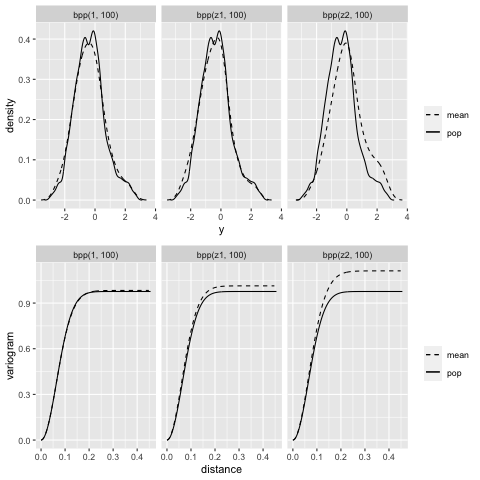
\includegraphics[width=0.7\textwidth]{fig/fig4.png}
\label{fig:sim_naive_est}
\end{figure}

%\begin{figure}[H]
%\caption{Relative Mean Squared Error to $\mathrm{bpp}(1, 100)$ of the variogram estimation}
%\label{fig:naive_est2}
%\centering
%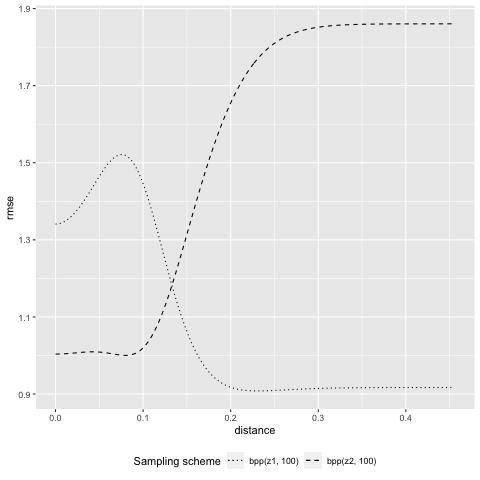
\includegraphics[width=0.6\textwidth]{fig/rmse.png}
%\end{figure}


\subsection{Maximum likelihood estimation}
%In particular, with ML we assume that the data $\Signal$ are multivariate Gaussian $(\textbf{X}\boldsymbol{\beta},{\color{red}\provar_{\position,\position^{'};\parampop}}$. The negative loglikelihood is {\color{red} FP: notation needs to be checked.} 
%{\color{red} DB: Can we just take the model with beta=0, Gaussian covariogram, $\parampop$ parameter of the covariogram (scale $\parampop_2$, and $\parampop_!=\sigma$).} 

%\begin{equation} \label{fit:ML}
%\likelihood\left(\boldsymbol{\beta},\parampop\right)=\left(n/2\right)\log{\left(2\pi\right)}+\left(1/2\right)\log{|\provar_{\position,\position^{'};\parampop}|}
%+\left(1/2\right)\left(\Signal-\textbf{X}\boldsymbol{\beta}\right)^{T}\provar_{\position,\position_{'};\parampop}^{-1}\left(\Signal-\textbf{X}\boldsymbol{\beta}\right)
%\end{equation}
%with estimators $\boldsymbol{\hat{\beta}}$ and $\hat{\parampop}$ satisfying $L\left(\boldsymbol{\hat{\beta}},\hat{\parampop}\right)=\inf{\lbrace L\left(\beta,\parampop\right):\boldsymbol{\beta}\in\mathbb{R}^{{\color{red}q}},\parampop\in\parampop\rbrace}$.

%\begin{equation} \label{fit:ML}
%\likelihood\left(\parampop\right)=\left(n/2\right)\log{\left(2\pi\right)}+\left(1/2\right)\log{|\provar_{\position,\position^{'};\parampop}|}
%+\left(1/2\right)\left(\Signal\right)^{T}\provar_{\position,\position_{'};\parampop}^{-1}\left(\Signal\right)
%\end{equation}
%with estimators $\hat{\parampop}$ satisfying $L(\hat{\parampop})=\inf{\lbrace L\left(\parampop\right):\parampop\in\parampop\rbrace}$.

Here we briefly present a possible solution that take into account the informativeness  of the sample. The proposal is based on the maximum likelihood estimation. In particular, in our setup, the loglikelihood of $\Signal[\position]$ is given by 

\begin{eqnarray} \label{Lnaive}
\likelihood_{\Signal[\position]}\left(\parampop;\signal\right)&=&\log(\density_{\Signal[\position]}(\signal;\parampop))\\&=&
\frac12\log{|\provar_{\position,\position^{'};\parampop}|}
+\frac12(\Signal[\Sample])^{\mathrm{T}}\provar_{\position,\position_{'};\parampop}^{-1}\Signal[\Sample]
\end{eqnarray}

and the naive estimator maximizes \eqref{Lnaive}. Indeed, this maximization ignores the selection mechanism. 

In order to take into account the informativeness of the sample, the \emph{full loglikelihood} should be used, which is composed by three factors: the density ratio, $\densityratio_{\Sample}(\position\mid\signal)$, the distribution of $\Signal$, $\density_{\Signal[\position]}(\signal)$, and the distribution of the sample, $\density_\Sample(\position)$. Therefore the loglikelihood is 

\begin{eqnarray} \label{fit:ML2}
\likelihood_{\Sample,\Signal[\Sample],\Samplesize}\left(\parampop,\paramnuisance;\position,\signal,\samplesize\right)&=&\log\left(\densityratio_{\Sample}(\position\mid\signal;\parampop,\paramnuisance)\right)+\log(\density_{\Signal[\position]}(\signal;\parampop))+\log\left(\density_\Sample(\position;\parampop,\paramnuisance)\right)
\end{eqnarray}

%{\color{red} Discuss here about what we do about $\density_\Sample(\position)$. Why we ignore it, although it may still contain information about $\theta$ and $\xi$, link to the debate about estimation in presence of nuisane parameters, reference to my draft paper and the approaches. Marginalisation or conditioning}


%REML estimators are obtained by applying maximum likelihood over error contrasts instead of the original data. %In the context of variogram estimation, the idea is to apply the likelihood over $\textbf{W}=\left(\Signal\left(1\right)-\Signal\left(2\right),\Signal\left(2\right)-\Signal\left(3\right),\dots,\Signal\left(n-1\right)-\Signal\left(n\right)\right)$
%Defining a vector of $n-\text{rank}\left(\Position\right)$ linearly independent (error) contrasts as $R=A^{T}\Signal$, where $A$ is an $\left(n-1\right)\times n$ matrix with elements
%\[
%a_{ij}=
%\begin{cases}
%1 &\text{for }i=j,j=1,\dots,n-1, \\
%-1&\text{for }i=j+1,j=1,\dots,n-1,\\
%0 &\text{elsewhere.}
%\end{cases}
%\]
%we have that $R\sim N\left(\textbf{0},A^{T}\provar_{\position,\position^{'};\parampop}A\right)$, which does not depend on $\boldsymbol{\beta}$. Moreover, if $A$ satisfies $AA^{T}=I-\Position\left(\Position^{T}\Position\right)^{-1}\Position^{T}$ and $A^{T}A=I$, we then have the following negative likelihood
%\begin{align*}
%L_{R}\left(\parampop\right)&=\left(\left(n-q\right)/2\right)\log{\left(2\pi\right)}-\left(1/2\right)\log{|\Position^{T}\Position|}+\left(1/2\right)\log{|\provar_{\position,\position^{'};\parampop}|}\\&+\left(1/2\right)\log{|\Position^{T}\provar_{\position,\position^{'};\parampop}^{-1}\Position |}+\left(1/2\right)\Signal^{T}\Pi\left(\parampop\right)\Signal
%\end{align*}
%where $\Pi\left(\parampop\right)=\provar_{\position,\position^{'};\parampop}^{-1}-\provar_{\position,\position^{'};\parampop}^{-1}\Position\left(\Position^{T}\provar_{\position,\position^{'};\parampop}^{-1}\Position\right)^{-1}\Position^{T}\provar_{\position,\position^{'};\parampop}^{-1}$ . Therefore, the REML estimate of $\parampop$ is obtained by minimizing $L_{R}\left(\parampop\right)$ over $\parampop$.




%Exact finite-sample distribution theory for estimators and corresponding variance estimators are available only in special circumstances (e.g. Jensen 1988). Therefore, simulations or approximation theory need to be employed in order to deal with intractable distribution theory. \cite{zimmerman1991comparison} presented a Monte Carlo comparison of different estimators, when two intrinsically stationary isotropic Gaussian random processes in $\mathbb{R}^{2}$ and various sampling intensities are taken into account. With regard to the MLE, different Authors agree that such approach can suffer from bias. \cite{warnes1987problems} illustrate potential problems by simulations of some simple spatial process, and \cite{mardia1989multimodality} indicate that these problems are caused by likelihoods not twice differentiable in $\parampop$. Moreover, a general conclusion that emerges from a set of several works based on simulations (Haining 1978c, Mardia and Meshall 1984, Swallow and Monahan 1984, Haining et al 1989, Zimmerman and Zimmerman 1991) is that the bias of MLE tends to be negative when the spatial dependence is positive, especially for small sample size. %{\color{red}and asymptotic variances of small-scale variation parameters are good approximation to exact variances only when the spatial dependence is weak.}

%For approximation theory, Cressie talks about two type of asymptotic theories {\color{red} pp }. \emph{Infill asympotics} refers to the the possibility to increase the sample size to infinity while the finite domain $D$ is kept fixed, whereas \emph{increase-domain asymptotics} refers to the situation where we take more units by means of increase the domain $D$. 

%Taken as it is from Cressie book (Section 7.3.1): when making inference on a random field $\lbrace Z(s):s\in D\rbrace$ from data $Z=(Z(s_{1},Z(s_{2}),\dots,Z(s_{n}))$, exact distribution theory of estimators, predictors, test statistics, and so on, is rarely available. Asymptotic distribution theory is the natural place to run for approximations, although, spatially, there are number of ways $n$ might tend to infinity.

%The \emph{naive estimated variogram} is 
%\begin{equation} \label{eq:g_hat}
    %\hat{G}(h)=\sum_{ij\in\Sample}{\beta_{ij}(h)(\Signal(\position_{i})-\Signal(\position_{j}))(\Signal(\position_{i})-Y(\position_{j}))^{T}}
%\end{equation}
%In equation \eqref{eq:g_hat}, the term $\beta_{i,j}$ is a mapping that may depend on the sample selected.
%Below we give possible definitions of $\beta_{i,j}$:
%\begin{equation}
    %\beta(\position_1,\position_2,h)=
    %\left|\begin{array}{l}
    %1 \text{ if } |\position_1-\position_2|=h, 0 \text{ otherwise}\\
    %\paramnuisance(\frac{|\position_{i}-\position_{j}|-h}{\alpha})
    %\end{array}\right.
%\end{equation},
%For binned estimation, a finite partition $(B_1,\ldots,B_n)$ of $\mathbb{R}^+$ is given as well as an element $h_k$ of each element $B_k$ of the partition. 
%Then the covariogram is first estimated for each $h_k$, as 
%...
%Then a covariogram is fitted 
%...
%In the following, we will not consider binned estimation.
%where {\color{red} $\paramnuisance$ is ..., and the bins $\mathrm{bin}_h=\left\{(i,j)\in\Sample^2\mid \left|\position_i-\position_j\right|\in [a_h,b_h)\right\}$}

%\subsection{Properties of the sample in the general case (including informative)}



 %Naive estimation of the population covariogram:
 %$E[naive~Covariogram]\neq$ pop cov,
 %$E[naive~Covariogram]=$ sample theoretical cov, 
 %with illustrative figures.




%\subsection{Parametric estimation}


\section{Prediction}
The variogram is a useful tool in order to quantify the spatial dependence in the data/process. Therefore, use of it in the inferential process has been investigated. We focus on the \emph{kriging} {\color{red} \citep{matheron1962traite}}, which is a minimum mean squared error method of spatial prediction that takes full advantage of the variogram. In fact, the kriging estimator incorporates the covariance structure of the $\Signal$ into the weights. In particular, the weights are based on the covariance among sample points and the covariance between sample points and predicted points. Note that this does not happen in distance-based method, where the weights depend only on the location of the points.

{\color{red} In the follow just some notes about ordinary kriging, it needs to be completed/reviewed}
\emph{Ordinary kriging} assumes following model
\begin{equation}
\Signal\left(\position\right)=\mu+\delta\left(\position\right)
\end{equation}
where $\position\in\mathbb{R}^{d}$, $\mu\in\mathbb{R}$, and $\mu$ unknown, and following predictor
\begin{equation}
P\left(\Signal,\Position\right)=\sum_{i=1}^{n}{\lambda_{i}\Signal\left(\position\right)}
\end{equation}
The weights $\lambda_{i}$s are computed such that the estimator is unbiased and the variance is minimized. {\color{red} Needs more here}


\subsection{Accounting for informative selection}


\appendix


\newpage
\section{Algebra for the example}
\subsection{Distribution of  $\Desvar$ conditionally on  $\Signal[\position]=\signal$}\label{sec:A.owifjoeij}
Under the condition of the paper example, conditionally on $\Signal[\position]=\signal$, the process $(\alpha+\beta\Signal+\gamma\varepsilon)$ is a Gaussian Process characterised by
$\mathrm{E}\left[(\alpha+\beta\Signal+\gamma\varepsilon)[\position']\right]=\alpha+\beta(\mu+\Sigma_{\position',\position}\Sigma_{\position,\position}^{-1} (\signal-\mu))$ and  $\mathrm{Var}\left[(\alpha+\beta\Signal+\gamma\varepsilon)[\position']\right]=\gamma^2\provar^\varepsilon_{\position',\position'}+\beta^2(\provar_{\position',\position'}-\provar_{\position',\position}\provar_{\position,\position}^{-1}\provar_{\position,\position'})$, and consequently, conditionally on $\Signal[\position]=\signal$, $\Desvar=\exp(\alpha+\beta\Signal+\gamma\varepsilon)$ is a lognormal spatial process.

%
%
%\begin{eqnarray*}
%\lefteqn{W[\position'_{1},\ldots,\position'_{m}]\mid\Signal[\position_{1},\dots,\position_{n}]=
%    \signal}\\&\sim&
%   P^{\alpha+\gamma\varepsilon[\position']}
%   \ast 
%    P^{\beta\Signal[\position']\mid\Signal[\position]=
%    \signal}\\&&=\ 
%   \mathrm{Normal}(\alpha+\beta(\mu+\Sigma_{\position',\position}\Sigma_{\position,\position}^{-1} (\signal-\mu)),
%\gamma^2\provar^\varepsilon_{\position',\position'}+\beta^2(\provar_{\position',\position'}-\provar_{\position',\position}\provar_{\position,\position}^{-1}\provar_{\position,\position'}))
%    \end{eqnarray*}

\begin{proof}

\begin{eqnarray}\lefteqn{\begin{bmatrix}
\Signal[\position']\\
\Signal[\position]
\end{bmatrix}\sim\mathrm{Normal}\left(\mu,\begin{bmatrix}\provar_{\position',\position'}&\provar_{\position',\position}\\
\provar_{\position,\position'}&
\provar_{\position,\position}
\end{bmatrix}\right)}\\
&\Rightarrow&
\left[
\left.\Signal[\position']
\right|
\Signal[\position]=\signal
\right]
\sim\mathrm{Normal}\left(\mu+\Sigma_{\position',\position}\Sigma_{\position,\position}^{-1} (\signal-\mu),\Sigma_{\position',\position'}-\Sigma_{\position',\position}\Sigma_{\position,\position}^{-1}\Sigma_{\position,\position'}\right)\label{eq:hfqopio}\end{eqnarray}

The independence of $\varepsilon$ and $\Signal$ implies that:
\begin{equation}\label{eq:iushfisduhsd}\left[\left.
\varepsilon[\position']
\right|
\Signal[\position]=\signal
\right]\sim\mathrm{Normal}\left(\mu_\varepsilon,\provar_{\position',\position';\varepsilon}\right),\end{equation} and that the vector obtained by stacking $\Signal[\position]$, $
\Signal[\position']$, and $\varepsilon[\position']$ is normal. 
By combining \eqref{eq:iushfisduhsd} and \eqref{eq:hfqopio} we obtain that:

$$\left[\left.\begin{bmatrix}
\Signal[\position']\\
\varepsilon[\position']
\end{bmatrix}\right|
\Signal[\position]=\signal
\right]\sim\mathrm{Normal}\left(\begin{bmatrix}\mu+\Sigma_{\position',\position}\Sigma_{\position,\position}^{-1} (\signal-\mu)\\0\end{bmatrix},
\begin{bmatrix}\Sigma_{\position',\position'}-\Sigma_{\position',\position}\Sigma_{\position,\position}^{-1}\Sigma_{\position,\position'}&0\\0&\provar_{\position',\position';\varepsilon}\end{bmatrix}\right).$$

We obtain the moments of $Z[\position']=\gamma
\varepsilon[\position']+\alpha+\beta
\Signal[\position']$ conditionally on $\Signal[\position]=\signal$:
$$\mathrm{E}\left[\alpha+\beta
\Signal[\position']+\gamma
\varepsilon[\position']|
\Signal[\position]=\signal\right]
=\alpha+\beta(\mu+\Sigma_{\position',\position}\Sigma_{\position,\position}^{-1} (\signal-\mu)),$$
and 
$$\mathrm{Var}\left[\alpha+\beta
\Signal[\position']+\gamma
\varepsilon\left[\position'\right]|
\Signal[\position]=\signal\right]
=\gamma^2\provar_{\position',\position';\varepsilon}+\beta^2\left(\provar_{\position',\position'}-\provar_{\position',\position}\provar_{\position,\position}^{-1}\provar_{\position,\position'})\right).$$
\end{proof}




\subsection{Algebra for $\provar$}

The denominator of $\rho$ requires the computation of $\int_{U}\Sigma_{\position',\position}~d\dominantU$, which is itself a function of
$\int_{U}\Covariogram(\position'-\position_j)d\dominantU\left(\position'\right)$


For $\position=(\position_1,\position_2)$, such that $\|\position_1-\position_2\|=h$, we have the following:

\begin{eqnarray*}
\Sigma_{\position,\position}&=&
    \begin{bmatrix}\Covariogram(0)&\Covariogram(h)\\\Covariogram(h)&\Covariogram(0)\end{bmatrix}\\
\Sigma_{\position,\position}^{-1}&=&
    (\Covariogram(0)^2-\Covariogram(h)^2)^{-1}\begin{bmatrix}\Covariogram(0)&-\Covariogram(h)\\-\Covariogram(h)&\Covariogram(0)\end{bmatrix}\\
\Sigma_{\position',\position}\Sigma_{\position,\position}^{-1}
    &=&(\Covariogram(0)^2-\Covariogram(h)^2)^{-1}
        \begin{bmatrix}\Covariogram(\position'-\position_1)&\Covariogram(\position'-\position_2)\end{bmatrix}\begin{bmatrix}\Covariogram(0)&-\Covariogram(h)\\-\Covariogram(h)&\Covariogram(0)\end{bmatrix}\\
    &=&\frac{\begin{bmatrix}
        \Covariogram(0)\Covariogram(\position'-\position_1)-\Covariogram(h)\Covariogram(\position'-\position_2)&              \Covariogram(0)\Covariogram(\position'-\position_2)-\Covariogram(h)\Covariogram(\position'-\position_1)\end{bmatrix}}{\Covariogram(0)^2-\Covariogram(h)^2}\\
\Sigma_{\position',\position}&=&\begin{bmatrix}\Covariogram(\position'-\position_1)&\Covariogram(\position'-\position_2)\end{bmatrix}
\end{eqnarray*}




\section{R code}


We generate a spatial Gaussian random process by means of the package \texttt{RandomFields}.


\bibliographystyle{apalike}
\bibliography{refs}

\url{https://warwick.ac.uk/fac/sci/statistics/staff/academic-research/nichols/research/spatbayes/johnson_spatialpointproc.pdf}

Kaar
Matheron.
Pfeffermann

\section{things deleted}

\sout{The sampling design could be very different according to the application, and could or not reflects some structure of the population. Every variable used in the selection is called \emph{design variable}. The \emph{probability proportional to size (pps)} sampling uses a variable $z$, or proxy variable, in order to select units  such that per each draw $k=1,...,n$, $P_{i}=P\left(I_{\position_{i}=1}\right)=z_{i}/\sum_{j=1}^{N}{z_{j}}$. The proxy variable has to be known for the entire population and usually it is correlated with the variable of interest. In this case the variable $z$ would be the design variable. For example, if interested in the level of specific pollutant, we could sample points with probability proportional to another variable correlated to it. In predicting areal rainfall, \cite{Kaar} considers that the points at which $Y$ is observed are the points $\position_{i}$ of a homogeneous two-dimensional Poisson process independent of $\Signal$. \emph{Spatially balanced sampling designs} select sample well spread over the area of interest, assigning low probabilities to be in the same sample to units close between them.}

{\color{red}
We need to add selected dots to the graph}




\appendix
\section{A kind of roadmap!}

    \paragraph{First step - simulation (done!)}
Illustrate through simulations the notion of sample variogram.\\
Setup:
\begin{itemize}    

    \item \textbf{simulation}: we use the dataset \texttt{meuse} as it were the population, compute the "real" variogram using all data, then sample by the selected sampling design and estimate the sample variogram;
    \item \textbf{code}: \url{https://github.com/DanielBonnery/Meuse}
    \item \textbf{results}: \url{https://github.com/DanielBonnery/Meuse/blob/master/demo/var_est.md}
\end{itemize}
\paragraph{Second step - theoretical development (to be done!)}
We need to model the spatial process $Y$ and $Z|Y$, with $Z$ spatial process of a design variable. From these, derive the distribution of 
\begin{itemize}
    \item $(I|Y,Z)$
    \item $(I|Z)$
\end{itemize}
then derive
\begin{itemize}
    \item $((Y(\textbf{x}_{1},Y\textbf{x}_{2})|I(\textbf{x}_{1})=I(\textbf{x}_{2})=1)$
\end{itemize}

The plan is:
\begin{enumerate}
    \item choose the covariance matrix for the spatial process $\Sigma(\theta,h)$, where $h$ is the distance;
    \item choose the design;
    \item express $\Sigma$ of sample;
    \item check that the estimated of the variogram bounces around theoretical sample variogram;
    \item derive results on the converge to sample variogram if possible.
\end{enumerate}



\section{Sketch}
The space $\Pop$ from which we sample from and a spatial process $Y:\Omega:\to \left(\Pop\to\range{Y}\right)$ with $\position\in\range{U}$, $\Cov\left(\Signal(\position_{1}), \Signal(\position_{2})\right)=\Semivariogram\left(\left|\position_{1}-\position_{2}\right|\right)$ and stationarity and isotropy assumption {\color{red}more on spatial model: dominated, fully parametric. Write density (likelihood of $Y$) with examples. Define f and g}

 $f(\position_1,\position_2,\signal_1,\signal_2)=\left(\mathrm{d}P^{\Signal(\position_1),\Signal(\position_2)}/\mathrm{d}\dominantY\right)(\signal_1,\signal_2)$
    
    we may limit ourselves to models such that exists $g$ such that 
    $\forall \position_1,\position_2,\signal_1,\signal_2$    $f(\position_1,\position_2,\signal_1,\signal_2)=g(\left|\position_2-\position_1\right|,\signal_1,\signal_2)$
    
Variogram:
\begin{equation}
    G(h)=E[(\Signal(\position+h)-\Signal(\position))((\Signal(\position+h)-\Signal(\position)))^{T}]
\end{equation}


Variogram:
\begin{equation}
    G(h)=E[(Y(\mathbf{x}+h)-Y(\mathbf{x}))((Y(\mathbf{x}+h)-Y(\mathbf{x})))^{T}]
\end{equation}

{\color{red}Define the sample here, define $I_{\position_1,\position_2}$}

Sample variogram:
\begin{equation} \label{somelabel}
    \hat{G}(h)=\sum_{ij\in\Sample}{\beta_{ij}(h)(Y(\mathbf{x}_{i})-Y(\mathbf{x}_{j}))(Y(\mathbf{x}_{i})-Y(\mathbf{x}_{j}))^{T}}
\end{equation}
In equation , the term $\beta_{i,j}$ is a mapping that may depend on the sample selected.
Below we give possible definitions of $\beta_{i,j}$:
\begin{equation}
    \beta(\position_1,\position_2,h)=
    \left|\begin{array}{l}
    1 \text{ if } |\mathbf{x}_1-\mathbf{x}_2|=h, 0 \text{ otherwise}\\
    \paramnuisance(\frac{|\mathbf{x}_{i}-\mathbf{x}_{j}|-h}{\alpha})
    \end{array}\right.
\end{equation},

For binned estimation, a finite partition $(B_1,\ldots,B_n)$ of $\mathbb{R}^+$ is given as well as an element $h_k$ of each element $B_k$ of the partition. 
Then the covariogram is first estimated for each $h_k$, as 
...
Then a covariofram is fitted 
...

In the following, we will not consider binned estimation.


where {\color{red} $\paramnuisance$ is ..., and the bins $\mathrm{bin}_h=\left\{(i,j)\in\Sample^2\mid \left|\position_i-\position_j\right|\in [a_h,b_h)\right\}$}

\begin{equation}
    E[\hat{G}(h)]=\sum_{i,j\in\Sampleindex}E\left[ \beta(\position_{(i)},\position_{(j)},h)(Y(\mathbf{x}_{(i)})-Y(\mathbf{x}_{(j)}))(Y(\mathbf{x}_{(i)})-Y(\mathbf{x}_{(j)}))^{\mathrm{T}}\right]
\end{equation}


In the case where $\beta_{\position_i,\position_j,h}$ is not random,

\begin{equation}
    E[\hat{G}(h)]=\sum_{\position_1,\position_2\in \Pop}{\beta()E\left[E\left[(Y(\mathbf{x}_{i})-Y(\mathbf{x}_{j}))^{2}|I\right]I(\position_1)I(\position_2)\right]}
\end{equation}

it is also equal to 


\begin{equation}
    E[\hat{G}(h)]=\sum_{\position_1,\position_2\in \Pop}{\beta()E\left[E\left[(Y(\mathbf{x}_{i})-Y(\mathbf{x}_{j}))^{2}|I(\position_1),I(\position_2)\right]I(\position_1)I(\position_2)\right]}
\end{equation}


Under certain conditions on the sample, for $i:\Pop\to\{0,1\}$, do we have 

\begin{eqnarray*}
\lefteqn{E\left[(Y(\mathbf{x}_{1})-Y(\mathbf{x}_{2}))(Y(\mathbf{x}_{1})-Y(\mathbf{x}_{2}))^T|I=i\right]}\\
&=&
E\left[(Y(\mathbf{x}_{1})-Y(\mathbf{x}_{2}))(Y(\mathbf{x}_{1})-Y(\mathbf{x}_{2}))^T|(I(\position_1),I(\position_2))=(i(\position_1),i(\position_2))\right]?\end{eqnarray*}

Let figure it out another day.


\begin{equation}
    E[\hat{G}(h)]=\sum{\beta()E\left[E\left[(Y(\mathbf{x}_{i})-Y(\mathbf{x}_{j}))^{2}|I\right]I\right]}
\end{equation}

\begin{equation}
\begin{split}
    \density_{(Y(\mathbf{x}_{1}),Y(\mathbf{x}_{2})|I(\position_1)I(\position_2)=1)}\left(\signal_1,\signal_2\right)&=\frac{\density_{Y(\mathbf{x}_{i}),Y(\mathbf{x}_{j})I(\position_1)I(\position_2)}(\signal_1,\signal_2,1,1)}{\int{f_{Y(\mathbf{x}_{i}),Y(\mathbf{x}_{j})I_{ij}}(y_{1},y_{2},1)}d y_{1}d y_{2}}\\
    &=\frac{\density_{Y(\mathbf{x}_{i}),Y(\mathbf{x}_{j})(\cdot,\cdot)}\cdot \density_{I(\position_1),I(\position_1)|(Y(\mathbf{x}_{1}),Y(\mathbf{x}_{2}))=(\signal_1,\signal(2))}(1,1)}{\int{f_{Y(\mathbf{x}_{i}),Y(\mathbf{x}_{j})I_{ij}(y_{1},y_{2},1)}d y_{1}d y_{2}}}\\
    &=\frac{\density_{Y(\mathbf{x}_{i}),Y(\mathbf{x}_{j})(\cdot,\cdot)}\cdot P(I(\position_1)I(\position_2)=1|(Y(\mathbf{x}_{1}),Y(\mathbf{x}_{2}))=(\signal_1,\signal_2)}{P(I(\position_1)I(\position_2)=1)}\\
    &=\rho(\signal_1,\signal_2)~\density_{Y(\mathbf{x}_{i}),Y(\mathbf{x}_{j})}(\signal_1,\signal_2) 
\end{split}
\end{equation}
\begin{equation}
    E[(Y(\mathbf{x}_{i})-Y(\mathbf{x}_{j}))^2|I_{ij}=1]
\end{equation}
Sample variogram: Property, under assumption (g assumption ...)
\begin{equation}
    \begin{split}
        \int{(Y(\mathbf{x}_{i})-Y(\mathbf{x}_{j}))^2dP^{Y(\mathbf{x}_{1}),Y(\mathbf{x}_{j})|I_{ij}=1}}=\int{\left(\signal_2-\signal_1\right)\left(\signal_2-\signal_1\right)^{\mathrm{T}}g(h,y_{1},y_{2})\rho(h,y_{1},y_{2})d y_{1} d y_{2}}
    \end{split}
\end{equation}

Sample distribution, for a given i

$$P^{(\Signal(\position))_{i(\position)=1}\mid I=i}$$


In order to understand the concept of informativeness, we need to distinguish between the population distribution and the sample distribution. In fact, as first definition, we say that a sample is informative if the distribution of the $y$ in the sample is different from the distribution of the $y$ in the population. In more detail, following \cite{pfefferman_1992}, the model holding on the sample can be different from the model holding in the population, due to selection mechanism. In particular, the joint pdf of all the available data is given by

\begin{equation} \label{eq:all_joint}
    f\left(\Signal_{s},\indicator,\Desvar;\theta,\paramnuisance,\rho\right)=\int{f\left(\Signal_{s},\Signal_{\bar{s}}|\Desvar;\theta_{1}\right)P\left(\indicator|\Signal,\Desvar;\rho_{1}\right)g\left(\Desvar;\paramnuisance\right)d\Signal_{\bar{s}}}
\end{equation}
while the pdf that does not take into account the selection mechanism is given by
\begin{equation} \label{eq:joint}
    f\left(\Signal_{s},\Desvar;\theta,\paramnuisance\right)=\int{f\left(\Signal_{s},\Signal_{\bar{s}}|\Desvar;\theta_{1}\right)g\left(\Desvar;\paramnuisance\right)d\Signal_{\bar{s}}}
\end{equation}
If the inference performed by \eqref{eq:all_joint} is equivalent to the inference performed by \eqref{eq:joint}, then the mechanism selection is said to be ignorable. A the contrary, we have an informative sample and we should take into consideration the selection mechanism in order to avoid the introduction of eventual bias in the final estimates.


{\color{red} delete this:\subsection{Sample Distribution of $\Signal$}




Conditionally on y, draw 1000 samples.
do non parametric logistic regression,
kernel: $E[I\mid Y]$ gives you an estimate of $\rho$.
Compute non parametric kernel regression estimator of $E[Z\mid Y=y]$.


\section{?}
\begin{eqnarray*}
\lefteqn{\Cov\left[\Desvar(\position'_1),\Desvar(\position'_2)\mid \left.\Signal\right|_{\{\position_{1},\dots,\position_{m}\}}=\signal
\right]}\\&=&2\provar^2_\varepsilon \left(\Semivariogram_\varepsilon(0)+\Semivariogram_\varepsilon(\position_2'-\position_1')\right)+\beta^2(
\provar_{\position'_1,\position'_2}-\provar_{\position'_1,\position}\provar_{\position,\position}^{-1}\provar_{\position,\position'_2})\\
&=& 2\sigma^2_\varepsilon \left(1+\Semivariogram_\varepsilon(\position_2'-\position_1')\right)+\beta^2(
(2(1+\Semivariogram_\Signal(\position'_2-\position'_1)-\provar_{\position'_1,\position}\provar_{\position,\position}^{-1}\provar_{\position,\position'_2})\\
&=& 2\left(\sigma^2_\varepsilon \left(1+\Semivariogram_\varepsilon(\position_2'-\position_1')\right)+\beta^2
\sigma^2_Y\left(\left(1-\Semivariogram_\Signal(\position'_2-\position'_1)\right)-\sum_{i,j=1}^n \left(1-\Semivariogram(\position'_1-\position_i\right)\left(1-\Semivariogram(\position'_2-\position_j)\right)B_{i,j}\right)\right)
\end{eqnarray*},

}



\begin{property}\label{Prop:1}
If 
[exchangeability condition on $\sampledensity_{\Sampleindex\mid \Desvar}(\position\mid \desvar)$] and 
[exchangeability condition on $P^Z$] 
then $\density_{\Sample[\Sampleindex]}(\position)=\dominantU(\Pop)^{-\#\Sampleindex}$.
\end{property}
\begin{proof}
Let show that $\density_{\Sample[\Sampleindex]}(\position)=\dominantU(\Pop)^{-\#\Sampleindex}$.
\begin{itemize}
\item[]
Let $\Sampleindex\subset\{1,\ldots,n\}$.
By definition $\density_{\Sample[\Sampleindex]}$ is a density on $\Pop^\Sampleindex$, so
$\int_{\Pop^\Sampleindex}\density_{\Sample[\Sampleindex]}(\position)\derive\dominantU^{\otimes\Sampleindex}(\position)=1$.
\item[]
Let show that $\density_{\Sample[\Sampleindex]}(\position)$ is constant.
\begin{itemize}
\item[]
Let assume that for any permutation $\permutation$ of

Let $\permutation$ be a permutation of $\{1,\ldots,N\}$. 
then $\sampledensity_{\Sampleindex\mid \Desvar}(\sigma.\position)=\int_{\DesvarSpace}\sampledensity_{\Sampleindex\mid \Desvar}(\sigma.\position\mid\desvar)\derive P^\Desvar(\desvar) $
\end{itemize}
\end{itemize}
Exchangeability with respect to $\dominantU$ of $....$ and $....$  implies the uniformity of the distribution of $\Sample$.
\end{proof}
When the conditions of Property \ref{Prop:1} hold, we have


\begin{equation}
\rho_{\Sampleindex}\left(\position \mid \signal\right)=
    \frac{\sampledensity_{\Sampleindex\mid \Signal[\Sample[\Sampleindex]]}\left(\position|\signal\right)}
    {\dominantU(\Pop)^{\#\Sampleindex}}.
\end{equation}



\end{document}


{\color{red}
$A=\provar_{\position,\position}$ is a symetric positive matrix:
$A=2\sigma^2_Y (\mathrm{I}-[\Semivariogram(|\position_j-\position_i|)]_{i,j})$
There exists $P$ orthogonal, $\Delta$ diagonal such that $A=^tP\Delta P$

Let $B$ be the inverse of $A$
}


